
\documentclass[Times,12pt,oneside,openany,print,index]{report}
\usepackage[a4paper,width=150mm,top=25mm,bottom=25mm]{geometry}
\usepackage[english]{babel}
\usepackage[utf8]{inputenc}
\usepackage{csquotes} % Provides advanced facilities for in-line and display quotations
\usepackage{amsmath} % TO use mathematical equations 
\pagestyle{plain} % Just a plain page number. For more http://www.emerson.emory.edu/services/latex/latex_129.html

\usepackage{graphicx} % to use the graphicx package
\graphicspath{/images} % Path to Image files 
\usepackage{caption} % To use caption with figure and images
\usepackage{array} % The array environment is used to make a table of information, with column alignment (left, center, or right) and optional vertical lines separating the columns

\usepackage[nottoc]{tocbibind} % The tocbibind package can be used to add the ToC and/or bibliography and/or the index etc., to the Table of Contents listing

\usepackage[normalem]{ulem} % The ulem package provides various types of underlining that can stretch between words and be broken across lines.

\usepackage{hyperref} % Provides LaTeX the ability to create hyperlinks within the document.
\hypersetup{
    colorlinks=true,
    linkcolor=black,
    filecolor=magenta,      
    urlcolor=black,
    citecolor=black,
}
\urlstyle{same}

\setlength{\parindent}{0em} % To control Indentation of paragraphs 

\usepackage{nomencl} % The nomenclature package can be used to generate and format a nomenclature using MakeIndex.
\renewcommand{\nompreamble}{The next list describes several symbols \& abbreviation that will be later used within the body of the document}
\makenomenclature

\usepackage[backend=biber,style=ieee,sorting=none]{biblatex} % for more plz click https://www.overleaf.com/learn/latex/Biblatex_citation_styles
\addbibresource{bibliography/references.bib} % Imports bibliography file

\let\cleardoublepage=\clearpage % removes unwanted doublepages
\usepackage{matlab-prettifier}
\usepackage{listings}
\usepackage{xcolor}
\definecolor{codegreen}{rgb}{0,0.6,0}
\definecolor{codegray}{rgb}{0.5,0.5,0.5}
\definecolor{codepurple}{rgb}{0.58,0,0.82}
\definecolor{backcolour}{rgb}{0.95,0.95,0.92}

\lstdefinestyle{mystyle}{
    backgroundcolor=\color{backcolour},   
    commentstyle=\color{codegreen},
    keywordstyle=\color{magenta},
    numberstyle=\tiny\color{codegray},
    stringstyle=\color{codepurple},
    basicstyle=\ttfamily\footnotesize,
    breakatwhitespace=false,         
    breaklines=true,                 
    captionpos=b,                    
    keepspaces=true,                 
    numbers=left,                    
    numbersep=5pt,                  
    showspaces=false,                
    showstringspaces=false,
    showtabs=false,                  
    tabsize=2
}

\lstset{style=mystyle}
\usepackage{matlab-prettifier}
\usepackage{multicol}
\usepackage{multirow}
\usepackage{rotating}
\usepackage{adjustbox}
\usepackage{geometry}
\usepackage{array}
\begin{document}

\thispagestyle{empty} % removes page number from title page
\begin{titlepage}
\renewcommand*{\thepage}{Title} % Change page number in PDF
\thispagestyle{empty}
\begin{center}
\vspace{3\baselineskip}
\begin{figure}[htbp]
\centering

\includegraphics[scale=0.05]{images/esisar_logo.png}
\hspace{7\baselineskip}
        
\includegraphics[scale=0.07]{images/schneider_logo.png}
\end{figure}

\vspace{-0.5\baselineskip} 
    { \Large \bfseries {Master in Integration, Security and Trust in Embedded systems} \par} 
    \vspace{\baselineskip} 
  \fbox { \Large {\bfseries {Graduation Project Report}} \par}

\fbox { \Large {\bfseries {Grenoble INP - Esisar 2022/2023}}\par}
 \vspace{\baselineskip}
 \vspace{\baselineskip}

  \vspace{\baselineskip} 

        {\large \bfseries \underline {Project Title}\par} 
\vspace{\baselineskip}
\large\bf {{ADS131M08 based electrical data acquisition and supervision with LTE-M, Matlab and Arduino cloud }\par}
    



\vspace{2\baselineskip}
    {\large \bfseries \underline {Name and address of company} \par}
\vspace{\baselineskip}
      {\large {Schneider Electric Industries} \par}
        {\large {31 Rue Pierre Mendes, 38320 Eybens, Grenoble, France} \par}
        
\vspace{2\baselineskip}
    {\large \bfseries \underline {Name and address of student} \par}
  \vspace{\baselineskip}
      {\large {MD. Shahnauze Ahsan} \par}
        {\large {2 Avenue des jeux olympiques, 38100, Grenoble, France} \par}

\vspace{2\baselineskip}
    \fbox {{\large \bf {Dates of Internship}} : {{February 2023 – July 2023}}}\par
    \fbox {{\large \bf {Speciality}} : {{ Integration of Embedded Systems}}}\par
    \fbox {{\large \bf Company Tutor} : {{Amine Hamza}}}\par
   \fbox {{\large \bf Esisar Tutor} : {{Ioannis Parissis}}}\par


%  \vspace{\baselineskip}
   


\vspace{2\baselineskip}
 {{École Nationale Supérieure d'Ingénieurs des Systèmes Avancés et Réseaux}\par}
    { \MakeUppercase{Grenoble INP - Esisar, UGA} \par}

 \end{center}


\end{titlepage} % Add title page
\cleardoublepage

\pagenumbering{roman} % Roman numbers to be use all pages before Chapter 1

%*******************************************************************
% TOC = Table of Contents
% The hyperref makes Title page No. 1 entry in the TOC
% In order to properly link  all section in TOC "phantomsection" command used
%  see below link for details on "addcontentsline"
% http://www.emerson.emory.edu/services/latex/latex_162.html
% "input" command to add files
% "Ethics Statement" & "Dedication" page are Optional; you may omit this two page if you want
% Please do not change the order of listings in TOC
%*******************************************************************

\phantomsection
\addcontentsline{toc}{chapter}{Abstract}
\section*{Abstract}
At Schneider Electric, engineers engaged in the development of AI algorithms require high-quality data samples. However, obtaining these data from the field presents challenges due to the limited connectivity of field products to the system. To address this challenge, this project proposes designing a ready-to-run acquisition system for monitoring electrical parameters such as voltage, current, temperature, and noise. This system will demonstrate high accuracy while operating efficiently on battery power, and it will establish a connection to the cloud using narrowband IoT technology, such as LTE-M. Subsequently, the acquired data will undergo analysis using local MATLAB and Simulink tools. Following the data analysis, our developed Simulink embedded algorithms will generate C code, which will then be seamlessly integrated into the firmware. This code will facilitate RMS measurements and anomaly detection for various loads.\par
\vspace{1cm}
\textbf{Keywords:} LTE-M; Arduino IoT Cloud; ADS131M08; Matlab; Data Acquisition
\pagebreak



\renewcommand{\contentsname}{Table of Contents} % Rename TOC name from Contents to Table of Contents
\cleardoublepage
\phantomsection
\addcontentsline{toc}{chapter}{Table of Contents} % Add Table of Contents in TOC
\tableofcontents % To  generation of the Table of Contents

\listoffigures % To  generation of the List of Figure
\listoftables % To  generation of the Tables of Figure

\printnomenclature % TO  generation of the Nomenclature file
\addcontentsline{toc}{chapter}{Nomenclature}
\cleardoublepage

\pagenumbering{arabic} % To use page number 1,2,3 ..

\chapter{Introduction}\label{introduction}
%\section{Introduction}
\section{Data Acquisition System} 
In recent years, a number of sectors, including process, fabrication, and automation, have adopted the practice of measuring, controlling, and testing equipment and processes utilizing computer systems and microprocessors. One such field that has been reinvented by the PC's rapid technical growth is data acquisition (DAQ), commonly known as DAQ. In order to collect, measure, store, and analyze data from diverse sources, a data acquisition system (DAS) combines hardware and software components. It makes it possible to gather actual signals or data from the outside environment and transforms it into a digital format for processing, analysis, and display. DAQ gear often handles the conversion of analog to digital signals as well as the reverse. The DAQ technology often works alongside a computer, such a standard PC. In this example, the computer is running DAQ software, which records and examines the data.



\vspace{0.5cm}
Data collection systems have evolved throughout time from electromechanical records with one to four channels to completely electronic architectures that can simultaneously measure hundreds of variables. In the early structures, the signals were continually recorded on paper graphs or magnetic tape rolls, but following the introduction of computers, especially personal ones, both the volume and speed of data collection substantially improved. The majority of conventional datalogger systems are still in use today, nevertheless. From straightforward setups with a few channels to complicated systems with hundreds or even thousands of channels, high-speed sampling rates, and networked architectures, data collecting systems can range in complexity and scalability.


\section{Core components of DAQ }
\textbf{Sensors and Transducers:}
Such devices soak up electrical or physical occurrences and turn them into signals. They might be flow meters, strain gauges, accelerometers, temperature sensors, pressure transducers, and many more.
\vspace{0.5cm}\par
\textbf{Signal Conditioning:}
It is frequently necessary to condition the sensor-acquired signals in order to assure their correctness, stability, and compatibility with the data collecting system. Amplifying, filtering, linearizing, calibrating, and isolating signals are some of the signal conditioning techniques.

\vspace{0.5cm}\par
\textbf{Analog-to-Digital Conversion:}
The incessant analog signals from the equipment's sensors are converted into digital data by analog-to-digital converters (ADCs) so that a computer or microcontroller may process it. The analog to digital converters (ADCs) create a digital representation of the signal amplitude by sampling the analog signals at predetermined rates.

\vspace{0.5cm}\par
\textbf{Data Acquisition Hardware:}
The hardware tools used to capture and process the digital data are included in this component. Usually, it contains cards or modules for data acquisition that are connected to the computer system and offer the analog input channels, digital input/output lines, and other characteristics needed for data collection.

\vspace{0.5cm}\par
\textbf{Data Acquisition Software: }
To manage the data acquisition process and operate the hardware for data collection, software programs or libraries are utilized. They offer interfaces for data viewing, analysis, and export and enable setup of sample rates, triggering mechanisms, and data storage choices.

\vspace{0.5cm}\par
\textbf{Data Storage and Analysis: }
The gathered data is kept for further analysis in computer systems, databases, or special storage devices. In order to get actionable insights from the collected data and make well-informed decisions, data analysis may use statistical techniques, signal processing algorithms, visualization tools, and other approaches.


\section{Aims and Objectives}
A multinational corporation, Schneider Electric focuses on providing automation and energy management solutions. Data acquisition systems (DAS) are essential in industrial settings for monitoring and managing operations, improving performance, maintaining quality, and assisting in decision-making. The aim of our project is to develop a ready to run acquisition system by using a multiple channel ADC which will be able for monitoring electrical parameters like voltage, current, temperature, and noise. This system will have high accuracy on battery and low power and will be connected to the cloud through wireless cellular communication technology.


\section{Outline}
Total nine chapters makes up the entire study of this project. Whereas the Corporate Social Responsibility has been discussed in chapter \ref{Corporate}. Some related works and state of arts has been narrated in chapter \ref{Literature}.Fundamental of ADC has been described in chapter \ref{Fundamental of ADC}. Numerous types of wireless IoT protocols and their performance map has been depicted in chapter \ref{Wireless IoT Protocols}. All the continuous development process of Hardware and Software implementation has been demonstrated in chapter \ref{Hardware} and chapter \ref{Software} respectively. The outcome of this project has been summarized in chapter \ref{Result}, and chapter \ref{Conclusion} represents the epilogue of this data acquisition system.




\nomenclature{$DAQ$}{Data acquisition}
\nomenclature{$DAS$}{Data acquisition system}
\nomenclature{$ADC$}{Analog-to-digital converter}


\chapter{Corporate Social Responsibility}\label{Corporate}
%\chapter{Corporate Social Responsibility}
\section{CSR Efforts}
The term "corporate social responsibility" (CSR) describes a company's efforts and deeds that go beyond its main business operations to benefit society, the environment, and its stakeholders. Like many big businesses, Schneider Electric has taken part in a number of CSR projects. The following are some broad areas where Schneider Electric has shown CSR efforts:

\begin{enumerate}
\item \textbf{Sustainability and Environmental Initiatives:} In order to lessen its carbon impact and advance environmental sustainability, Schneider Electric has made a commitment. This includes actions taken in its own operations as well as through its solutions and products to increase energy efficiency, lower greenhouse gas emissions, and encourage the use of renewable energy sources.

\item \textbf{Access to Energy: }Schneider Electric has started programs to give underprivileged people, particularly those in developing areas, access to dependable and sustainable electricity. This is in line with the Sustainable Development Goal (SDG) of the United Nations to ensure that everyone has access to modern, cheap, dependable, and sustainable energy.

\item\textbf{Ethical Business Practices:} CSR also includes moral business conduct including fostering openness, honesty, and ethical company governance. In the nations where it conducts business, Schneider Electric has probably made efforts to guarantee adherence to legal and regulatory requirements.

\item\textbf{Diversity and Inclusion:} Companies frequently make efforts to encourage diversity and inclusion among their employees and in their communities. This may entail initiatives to empower minority groups, advance gender equality, and develop equitable opportunity.

\item\textbf{Community Engagement:} Various community involvement and social development initiatives have been undertaken by Schneider Electric. Supporting regional projects for healthcare, education, and other community-based efforts might fall under this category.

\item\textbf{Circular Economy and Waste Reduction:} Schneider Electric's CSR activities also include programs to promote a circular economy and lessen waste. This can entail making products durable and recyclable.

\item\textbf{Partnerships and Collaboration:} To increase the effect of many CSR activities, partnership with philanthropic groups, governmental organizations, and other stakeholders is used.

\end{enumerate}

\section{Contribution to SDG}
In support of various Sustainable Development Goals (SDGs) set forth by the United Nations, Schneider Electric has been actively involved. The following implications of our initiative on the achievement of these SDGs are listed: 


\begin{enumerate}

\item\textbf{SDG 7- Affordable and Clean Energy:} The company's products and services help improve energy efficiency, promote the use of renewable energy sources, and provide access to reliable and sustainable energy, contributing to SDG 7's goal of ensuring affordable and clean energy for all. Our IoT based data acquisition system can assist in optimizing energy consumption, improving energy efficiency, and integrating renewable energy sources.

\item\textbf{SDG 9 - Industry, Innovation, and Infrastructure:} Schneider Electric's technologies and solutions play a significant role in advancing industrial automation, digital transformation, and infrastructure development. Their focus on innovation helps drive efficiency and sustainability across industries, contributing to SDG 9. A well-implemented DAS can enhance industrial processes, improve manufacturing efficiency, and facilitate innovation by providing real-time data insights. This can lead to more sustainable and efficient production methods, contributing to SDG 9's focus on building resilient infrastructure and promoting sustainable industrialization.

\item\textbf{SDG 11 - Sustainable Cities and Communities:} Schneider Electric's smart city solutions contribute to creating more sustainable and resilient urban environments. These solutions include smart grid technologies, energy-efficient building systems, and integrated urban infrastructure management. Our implemented data acquisition system can be employed to gather data related to urban infrastructure, and load management. Because of having remote maintenance feature in our project, zero carbon emission goals is being achieved, which is contributing to the goals of SDG 11


\item\textbf{SDG 12 - Responsible Consumption and Production: }Schneider Electric promotes responsible consumption and production through its efforts to improve energy efficiency, reduce waste, and support the transition to a circular economy. Their commitment to eco-design and product lifecycle management aligns with this goal. Data acquired through a DAS can help monitor resource consumption, waste generation, and production efficiency. By optimizing processes and reducing waste, companies can contribute to more responsible consumption and production patterns, orienting with SDG 12.

\item\textbf{SDG 13 - Climate Action:} The company's focus on energy efficiency, renewable energy, and reducing carbon emissions directly contributes to SDG 13's objective of combating climate change and its impacts. DAS can play a crucial role in monitoring environmental parameters such as air quality, noise, temperature, and emissions. Accurate and timely data collection can support climate change mitigation and adaptation efforts, helping to achieve the objectives outlined in SDG 13.

\end{enumerate}

\vspace{0.5cm}

Finally, Schneider Electric's Corporate Social Responsibility (CSR) initiatives stand out as evidence of the business' steadfast commitment to making the world a better place. They have successfully incorporated sustainability into their fundamental business processes through a thorough and forward-thinking strategy, going beyond simple compliance and embracing a greater purpose. Schneider Electric's dedication to social advancement, environmental protection, and moral behavior highlights their responsibility as a corporate citizen. Schneider Electric exemplifies how a global leader can generate good change while promoting innovation and cooperation by supporting programs that span from energy efficiency and renewable solutions to community empowerment and ethical governance.Schneider Electric continues to innovate and set an example for businesses throughout the world, demonstrating that social responsibility and commercial success are not incompatible but rather go hand in hand as we move toward a more sustainable and inclusive future.







\nomenclature{$CSR$}{Corporate Social Responsibility}
\nomenclature{$SDG$}{Sustainable Development Goals}
\chapter{Literature Review}\label{Literature}

%\chapter{Literature Review}
Over the past few decades, significant advancements have been made in DAS technology. The transition from analog to digital data acquisition has allowed for improved accuracy, reliability, and ease of data manipulation. Additionally, the integration of microprocessors and programmable logic devices has led to the development of smart and autonomous data acquisition solutions. Moreover, wireless and remote sensing capabilities have expanded the scope of data collection to remote or hazardous environments, enhancing the flexibility and accessibility of DAS. In this chapter we will discuss some state of arts what we have studied during our research work.
\vspace{0.5cm}\par
Sarra Houidi et al \textbf{\cite{Load_Monitoring}} introduces a study about an economical current and voltage measurement system, employing an Arduino MKR Zero microcontroller, aimed at facilitating Non-Intrusive Load Monitoring for Home Electrical Appliances. The hardware architecture is thoughtfully outlined, encompassing current and voltage conditioning circuits, while the software aspect is comprehensively detailed. The microcontroller's interruption routine ensures consistent data acquisition, complemented by a background task for efficient data storage using a micro SD card. The authors also envision future enhancements, including potential networking capabilities for consumer accessibility via web interfaces, along with the ability to extend the system's applicability to measuring currents and voltages within domestic three-phase networks. We have choosen Arduino MKR 1500 for our project, but we used ADS131M08 delta-sigma ADC where they utilised some operational amplifiers to serve the purpose. They have stored their data into a micro SD card, where we stored it in Arduino IoT cloud.

\vspace{0.5cm}
Another research has been conducted by Hendrik et al \textbf{\cite{MADV-DAQ}} in the past for structural health monitoring of onshore wind turbines and wind turbine foundations. It is an affordable, multi-channel, Arduino-based differential voltage data collection device appropriate for battery-operated measurements of several Wheatstone bridge-based (strain) sensors from distant locations. In this system The Arduino microcontroller serving as the main data acquisition device, with an additional Raspberry Pi transferring the data to two other data hubs for long-term preservation and analysis. Our system was also designed in Arduino platform, but we didn't developed our local data storage server. Because we were envisioned to design something low cost and affordable. 
\vspace{0.5cm}

In a project of Sadia et al, \textbf{\cite{Portable_Sensing}} a multimetric, low-power-consumption sensor system was developed for real-time data acquisition. The finite element analysis aims to determine the strain gauge positions at which the strain is zero during the lifting stage. The general strategy of precast monitoring is validated by conducting an experiment in which the delivery of a 12-m-long PCS is monitored using the PDMS. In addition, a safety evaluation strategy was developed to assess the maximum strain on the structure by using offset-adjusted strain measurements. Their system was based on Teensy 4.1 micro-controller and ADS131M08 ADC, with an OpAmp and 3 axis accelerometer. For data storage they have utilised an SD card. On the other hand, our system was based on Arduino and real time cloud connected.

\vspace{0.5cm}
Yuguang Fu et al \textbf{\cite{Event_Monitor}}, developed wireless sensors that conserve battery power through duty-cycling. However, this approach may miss sudden events while in power-saving sleep mode. To enable continuous monitoring, they proposed a sustainable power solution emulating wired systems. By using a trigger node or system, the sensors can be continuously monitored, ensuring timely event notification to the power-saving nodes. The proposed wireless sensor system (WSS) demonstrated low power consumption, drawing only 365 A without sudden events, compared to 170 mA for the original sensor platform. This extended the lifetime of always-on monitoring when using a rechargeable lithium polymer battery. In field tests, the WSS was evaluated on a steel railroad bridge and performed well for earthquake monitoring and sudden event detection. Additionally, the sensors offered high sampling rates and sensing resolution, providing high-quality data for rapid condition assessment of civil infrastructure during sudden events. We took the idea for adding rechargeable lithium polymer battery in our system after this study. Though we have selected 24 bit ADC which provide better sampling rate than theirs 12 bit ADC.

\vspace{0.5cm}
Some researchers in \textbf{\cite{WireLs_SmartSensor}}demonstrated the potential of WSS platforms for high-fidelity Structural Health Monitoring (SHM) applications. They compared several WSS platforms, including Martlet AX-3D, Waspmote v15, and G. Link-200, based on critical requirements from standards and full-scale deployments. Their study found that the AX-3D had milliseconds time synchronization errors, which could lead to false indications of structural damage during condition assessment. To support large-scale, high-fidelity sensing, the Xnodes underwent hardware improvements, including high-speed microprocessors, high-resolution sensors, powerful wireless communication, and efficient power management. Extensive lab and field tests validated the Xnodes performance in data acquisition, wireless communication reliability, and power management efficiency. They have defined three different tasks in FreeRTOS. After studying these research work we got the motivation to implement an OS in owr system, where we have defined four different tasks will be described later.

\vspace{0.5cm}
In the research of Krzysztof Sieczkowski et al \textbf{\cite{RealTimeAcq_Matlab}}, build a real-time data acquisition method utilizing Matlab software for external devices. It introduces a communication protocol and transfer framework ensuring reliable interaction between the master system and external measuring sensors. The study encompasses a detailed description of a measurement station implementing this protocol, alongside a comprehensive algorithm for test programs.Three performance tests were conducted, focusing on key aspects: (1) average transmission time, (2) effective throughput of complete data exchange cycles, (3) Matlab's processing time for transmission, and (4) stability of the program timer for periodic data transmission calls. The experimentation incorporated three widely used communication interfaces (UART, Bluetooth, WiFi) and diverse packet sizes.\par
\vspace{0.5cm}
Some scholars in \textbf{\cite{OpenAcq_Matlab}} provides insights into seamless real-time data acquisition, offering a systematic assessment of performance across various communication interfaces and packet sizes. This study introduces an innovative and cost-effective data acquisition system that leverages open-source hardware in conjunction with Matlab/Simulink. This system offers the unique capability to acquire a diverse range of data types and sample rates, utilizing both USB and serial communication methods. The hardware foundation is established with Arch Max, featuring an ARM Cortex-M4 core. The software architecture includes microcontroller firmware presented as a user-friendly header file, streamlining data acquisition via readily accessible functions.
\vspace{0.5cm}

Anshuman Panda et al \textbf{\cite{Matlab_DAQ}} introduces a software platform that employs Matlab and Simulink for economical data acquisition and control tasks through low-cost microcontrollers. Designed for applications requiring graphical user interfaces (GUI) and advanced computation without demanding hardware specifications, the framework is exemplified through DC motor position control using a Basic Stamp 2 (BS2) microcontroller alongside the Matlab data acquisition and control toolbox. We have also designed an embedded algorithm in our system to analyse the acquired data.
\vspace{0.5cm}

The research paper of J. Krizan et al \textbf{\cite{Automatic_code}}, investigates the utilization of automatically generated C-code from the Matlab and Simulink environment in critical applications aligned with DO-178C and DO-331 standards. Employing Model Based Design, the study showcases how algorithms initially tested as models can be seamlessly translated into C-code, reducing potential errors associated with manual coding. The focus lies in examining the practicality of this model-based approach for critical avionics applications, aiming to meet MISRA-C software standards. This study helps us to implement C code from our simulink embedded algorithm.



\nomenclature{$PDMS$}{Precast Delivery Monitoring
System}
\nomenclature{$WSS$}{Wireless Sensor System}
\nomenclature{$SHM$}{Structural Health Monitoring }
\nomenclature{$UART$}{Universal Asynchronous Receiver Transmitter}




































\chapter{Fundamental of ADC}\label{Fundamental of ADC}

%\section{Fundamental of ADC}
\section{ADC principles} 
The majority of the events that happen around us and the signals that various types of sensors collect are analog in form. Through the processing of these analog signal information can be extracted. Both the analog space or digital domain could be utilized in signal processing. In comparison with analog signal processing, digital signal analysis provides a variety of benefits, including reduced noise sensibility, better design autonomy, the capacity to apply advanced digital filters, simpler compressing data and archiving, etc. All of the aforementioned advantages motivate an impulse to convert analog signals to digital signals. 
\vspace{1\baselineskip}\par 
Digital data signals are generated from analog ones via analog-to-digital converters. To do this, the analog signal is approximated by a finite amount of digital values shown in figure \ref{fig:x Conversion)}. The analog signal undergoes sampling with a constant period of time prior to performing this modification. As a consequence, the signal that was analog is discrete both for time and magnitude in a digital illustration of it. A typical conversion has been depicted in figure \ref{fig:x Conversion series)}. In this illustration, the source signal first goes through an anti-alias filter. We know aliasing occurs when a signal is sampled at a lower resolution than the original, resulting in distortion, jagged edges, or false patterns. The purpose of an anti-aliasing filter is to remove or reduce high-frequency components in a signal before it is sampled. In figure the signal is then sampled utilizing a sample-and-hold (S/H) circuitry before being sent to a quantizer, which approximates the magnitude of the signal.
\vspace{1\baselineskip}\par 
The following may be expressed as the relationship between an analog and digital signal:

\begin{align}
    V_{in} = D_{out}q_n + e_q
\end{align}

Here $D_{out}$ is the ADC's digitized output, $q_n$ is the quantization step, and $e_q$ represents the quantization error, or the discrepancy between the analog signal and its corresponding digital representation.

\begin{figure}[htbp]
\centering
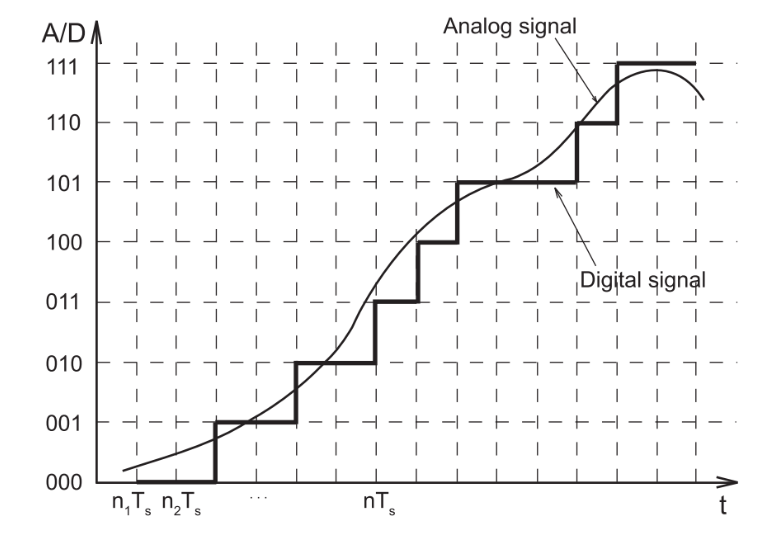
\includegraphics[scale=0.5]{images/ADC.png}
\caption{Analog to Digital Conversion}
\label{fig:x Conversion)}
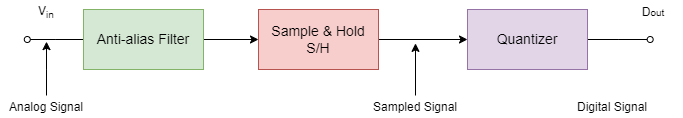
\includegraphics[scale=0.5]{images/ConversionChain.png}
\caption{Analog to Digital Conversion series}
\label{fig:x Conversion series)}
\end{figure}

\section{ADC Characteristics}
ADCs have various characteristics and parameters that define their performance and behavior.  These characteristics are crucial for understanding the capabilities and limitations of an ADC. We have studied several books and articles \cite{ADC_Param},\cite{Acquistion_Eren},and \cite{DAQ_Fundamental} to explore the ADC fundamental, characteristics and parameters. Some of this gist are listed below:
\vspace{1\baselineskip}\par 
\textbf{Resolution:} Resolution is one of the most critical characteristics of an ADC. It refers to the number of bits in the digital output code produced by the ADC. A higher resolution means more bits and greater precision in representing the analog signal. The resolution determines the number of discrete levels or steps into which the ADC can divide the input voltage range. It is the proportion of the change in the input analog voltage to the change in the digital output by one LSB.
\begin{align}
    Resolution = V_{FS} / 2^n -1
\end{align}
Here, $V_{FS}$ is the Full scale input voltage, and n is the number of bit for ADC.
The resolution of a measurement influences its accuracy. The measurement data are more accurate the higher the digitizer resolution. Let's look at what a waveform might be like after being processed by digitizers with various resolutions. Figure \ref{fig:x Resolution Comparison} illustrates the responses of 12, 14, and 16 bits of a typical digitizer to a section of a 200 mV damped sine waveform.

\begin{figure}[htbp]
\centering
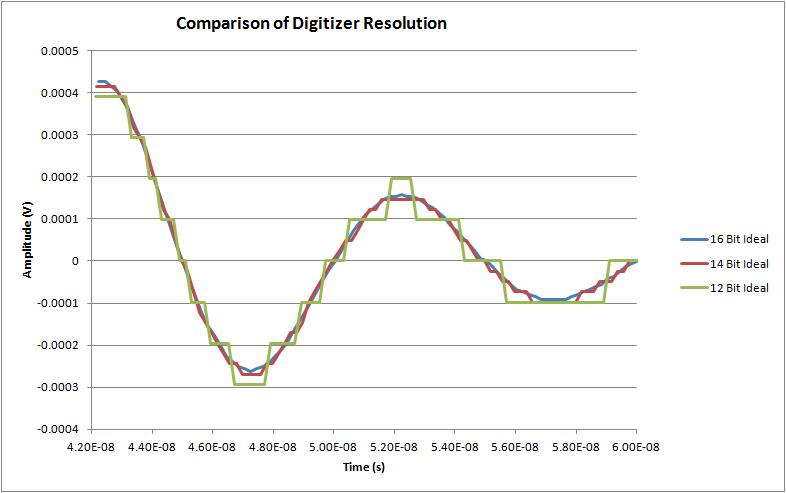
\includegraphics[scale=0.4]{images/Resolution.png}
\caption{A comparison of digitizer resolution on measurement precision}
\label{fig:x Resolution Comparison}
\end{figure}

\vspace{1\baselineskip}\par 
\textbf{Sampling Rate:} The sampling rate is the number of samples taken per unit time by the ADC. It represents how frequently the ADC captures the analog signal. The sampling rate is typically measured in samples per second (SPS) or kilohertz (kHz). A higher sampling rate allows the ADC to capture and represent higher-frequency components of the analog signal accurately. To satisfy the Nyquist-Shannon sampling theorem, the sampling rate must be at least twice the highest frequency component present in the analog signal. This ensures that the digital samples can accurately represent the original analog signal without introducing aliasing or loss of information. For example, if an analog signal contains frequency components up to 10 kHz, the ADC should have a sampling rate of at least 20 kHz to avoid aliasing and accurately capture the signal. The choice of sampling rate depends on the requirements of the application. Higher sampling rates are necessary for accurately capturing high-frequency signals or for applications that require fine time resolution. However, higher sampling rates also result in increased data processing and storage requirements.

\vspace{1\baselineskip}\par 
\textbf{Accuracy:} The ADC's accuracy measures how closely the digital output corresponds to the actual analog input. Numerous elements, including linearity, gain error, offset error, and noise, have an impact on it. There won't be many differences or mistakes between the input and output values of an accurate ADC. The least significant bits (LSBs) or a percentage are commonly used to describe an ADC's accuracy.

\vspace{1\baselineskip}\par 
\textbf{Linearity:} The level of linearity in an ADC refers to how closely the analog input voltage and matching digital output code follow a straight line connection. For similarly spaced analog input voltages, the ADC should generate consistently spaced digital steps. The ideal transfer function may, however, deviate due to flaws in the ADC that cause nonlinearity. Integral nonlinearity (INL) or differential nonlinearity (DNL), which measure the greatest departure from the ideal transfer function, are frequently used to measure the linearity of an ADC.

\vspace{1\baselineskip}\par 
\textbf{Gain Error:} The gap between the ADC's real gain and its ideal gain is known as gain error. Scaling mistakes are introduced into the digital output code. Gain error is frequently quantified in terms of LSBs or percentages.

\vspace{1\baselineskip}\par 
\textbf{Offset Error:} Offset error is the difference between the actual zero-voltage intercept and the transfer function of the ADC. It can be represented as a voltage or LSB value and reflects an added error to the measured value. When there is no input signal, offset error is what causes the offset or shift in the digital output code.

\vspace{1\baselineskip}\par 
\textbf{Signal-to-Noise Ratio:} SNR is a metric that expresses the strength of the intended signal in relation to the noise level at the ADC output. Decibels (dB) are frequently used to express it and are used to measure the amount of noise in the digital output. Better signal integrity and lower noise levels are indicated by a greater SNR.

\vspace{1\baselineskip}\par 
\textbf{Total Harmonic Distortion:} The amount of harmonic distortion the ADC introduces when converting an analog signal to a digital signal is measured by THD. When there are additional frequency components in the output signal that weren't in the analog signal's original version, it's known as harmonic distortion. The amount of distortion in the digital output is indicated by THD, which is given as a percentage or in dB.


\section{ADC architectures}
There are several distinct ADC designs that may be employed for certain application requirements. They are characterized by the rate of sampling or the total amount of clock cycles required to convert a single digital word and resolution. After studying the research paper \cite{KozminPhD}, we have acknowledged that ADC designs are commonly classified into four groups based on sample speed, which has been specified below.
\vspace{1\baselineskip}\par 
\textbf{Slow ADC:} Integrating ADCs have the slow converting speed (2N clock oscillations per data word) but the greatest resolution, which is often greater than 14 bits.\par

\textbf{Medium ADC:} To convert a single sample, a sequential approximations ADC needs N clock cycles. The possible resolution is in the 8-14 bit range.
\par

\textbf{Fast ADC:} This category includes flash, pipeline, subranging, and time-interleaved ADCs. One sample is converted in one to two clock periods. These ADCs generally have resolutions ranging from 6 to 12 bits.\par

\textbf{Oversampling ADC:} Oversampling ADCs, also known as noise- forming ADCs, utilize delta-sigma. Its conversion speed and resolution fall in between those of slow and medium ADCs.\par
\begin{figure}[htbp]
\centering
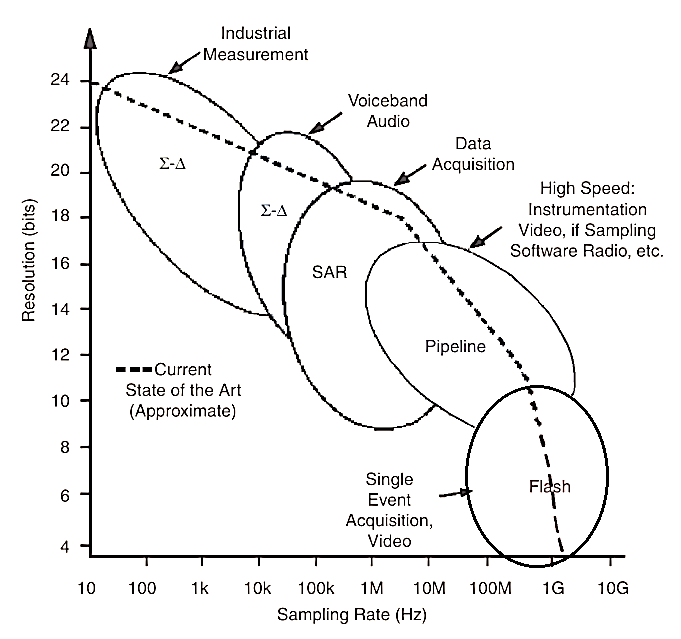
\includegraphics[scale=0.6]{images/ADC Archi.PNG}
\caption{ADC architectures, applications, resolution, and sampling rates.}
\label{fig:x ADC architectures}
\end{figure}

\subsection{Integrating ADC}
There are two techniques to realizing integrating ADCs: single slope and dual slope.These two ADCs interact by integrating a continuous reference signal. Dual Slope ADCs employ integration techniques to calculate the input voltage by measuring the time required for charging or discharging a capacitor. ADCs with dual slopes give high-resolution readings with outstanding noise suppression. They integrate upwardly from an unidentified voltage and then downwards with a knowing voltage source.These are more precise than single sloped ADCs, becuase component defects are wiped away during the de-integration process.Figure \ref{fig:x Dual Slope} is an illustration of slope integration. This charges a capacitor with an electrical current equal to the input voltage over a specific amount of time. The time needed for discharging the identical capacitor at a constant current then establishes the input voltage value. Since it is based on the proportion of ascending time to descent time rather than the true value of the capacitor or other elements whose values fluctuate with temperature and time, the approach is generally precise and reliable.

\begin{figure}[htbp]
\centering
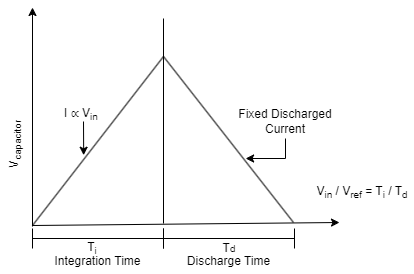
\includegraphics[scale=0.6]{images/Slope.png}
\caption{Dual-Slope ADC Integration and
Discharge Times}
\label{fig:x Dual Slope}
\end{figure}

While an integration timing matches to a multiple of the ac periods, the impact of noise pickups on the ac line's frequency is reduced through integrating the ADC input over an interval. It is frequently utilized in panels meter and precise digital multimeters because to this. Even while conversion rates of up to 60 Hz are typical for 20-bit accuracy, they can be slower for ADCs that integrate across multiples of the line frequencies.

\subsection{Successive-Approximation ADC}
A digital-to-analog converter (DAC), one comparator, controlling logic, and registers make up a successive-approximation converter (Figure \ref{fig:x Successive-Approximation ADC}). The logic initializes the DAC to zero before beginning to count up and set each bit after that until it's reached the current state of the input voltage being monitored \cite{DAQHandbook}. The final value is then recorded in the register when the conversion is complete.The system's logic for control first sets every bit to zero whenever the analog voltage that needs to be assessed is present at the comparator's input.The DAC's output is therefore forced to Half of full scale (as an example of a 10 V full-scale system, the DAC outputs 5.0 V) when the most significant bit (MSB) is set to 1.The comparator subsequently evaluates the analog result of the DAC and compared it to the incoming signal; if the output of the DAC is less than the input signal (which is the signal is more than 1/2 full scale), the MSB is kept at 1.The MSB restores to zero when the output of the DAC is greater than the input signal. Following that, the second MSB, which has a weight of 1/4 of full scale, goes on (sets to 1) and pushes the output signal of the DAC to either 3/4 full scale (if the MSB stayed at 1) or 1/4 full scale (if the MSB restore to zero).Another time, the comparator checks the DAC output to its input signal; if the DAC output is greater than the input, the subsequent bit is reset to zero; otherwise, it remains on (sets to 1). The method then proceeds in order of decreasing bit weight till the LSB is contrasted, after which the 3rd MSB is compared in a similar fashion. The resultant register stores the digital code that represents the analog input signal at the final stage of the procedure.

\begin{figure}[htbp]
\centering
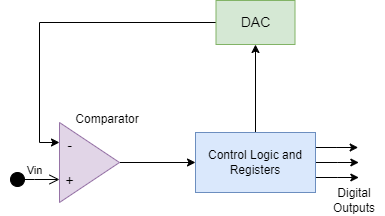
\includegraphics[scale=0.6]{images/SAD.png}
\caption{Successive-Approximation ADC}
\label{fig:x Successive-Approximation ADC}
\end{figure}
Comparisons are performed serially in Successive-Approximation ADC,also they must pause after each step to initialize the DAC and wait for its output to stabilize. Thats why these ADCs are relatively slow.Progressive approximation Because comparisons are performed serially, ADCs are rather sluggish because they must pause after each step to initialize the DAC and wait for its output to stabilize. However, the rate of conversion frequently exceed 1 MHz. Additionally, 12 and 16-bit successive-approximation ADCs are affordable, which explains their widespread use in numerous PC-based collection systems.


\subsection{Flash ADC}
A bunch of parallel connected comparators ($2^N-1$) shown in figure \ref{fig:x Flash ADC}, each with a unique reference level constructs flash ADC.
\begin{figure}[htbp]
\centering
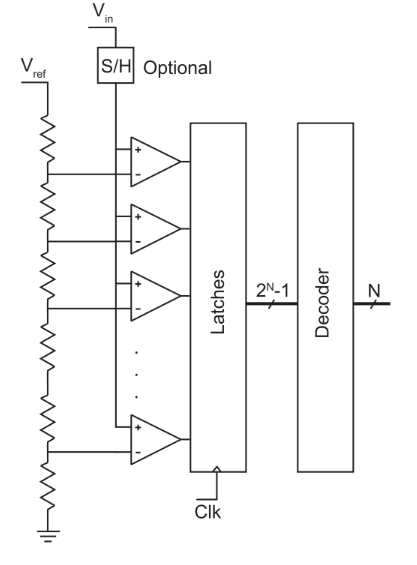
\includegraphics[scale=0.6]{images/Flash.PNG}
\caption{Flash ADC structure}
\label{fig:x Flash ADC}
\end{figure}
The output of the comparator arrays resembles a thermometer because it includes $2^N-1$ bits for every comparator, and each One indicates that the signal is higher than the associated reference value. Afterwards, the decoder converts this code into a binary format. The core component of a Flash ADC is an array of high-speed comparators. Each comparator in the array compares the input analog voltage with a set of reference voltages.The number of comparators in the array directly determines the ADC's resolution.The outputs of the comparators represent the comparison results. For instance, if the input analog voltage is greater than the reference voltage of a comparator, the output is a digital '1'; otherwise, it is a '0'.
\vspace{1\baselineskip}\par 
Flash ADCs are capable of achieving very fast conversion rates, making them suitable for applications requiring high-speed signal processing. They have low conversion latency, which is important in real-time signal processing systems.They can achieve high resolution since each comparator bit contributes to the overall ADC resolution. As the resolution of the ADC increases, the number of comparators and power consumption also increase significantly. Despite its many advantages, Flash ADC has several drawbacks.As the ADC resolution grows, the number of comparators and required precision of the reference voltages become challenging to manage.
\subsection{Delta-sigma ADC}
A high-resolution ADC, known as a Sigma-Delta ADC exploits the oversampling approach to obtain high accuracy in the conversion of analog data to digital format. It consists of a comparator, an integrator, a DAC, and a summing junction, shown in figure \ref{fig:x Delta-sigma ADC} . The fundamental operation of a Sigma-Delta ADC incorporates oversampling the analog input signal at a very high sampling rate, then applying a digital filter to remove noise and retrieve the important data. The digital output data is then generated from the filtered output via decimation.

\begin{figure}[htbp]
\centering
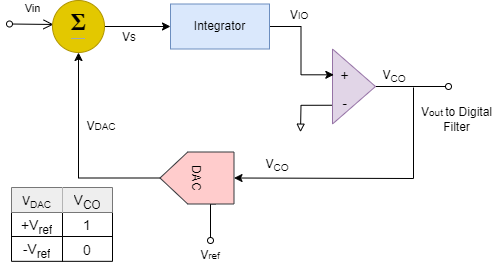
\includegraphics[scale=0.6]{images/Sigma.png}
\caption{Delta-sigma ADC structure}
\label{fig:x Delta-sigma ADC}
\end{figure}





\nomenclature{$LSB$}{Least Significant Bit}
\nomenclature{$SPS$}{Samples Per Second}
\nomenclature{$dB$}{Decibel}
\nomenclature{$SNR$}{Signal-to-Noise Ratio}
\nomenclature{$THD$}{Total Harmonic Distortion}
\nomenclature{$DAC$}{Digital-to-analog converter}
\nomenclature{$MSB$}{Most significant bit}

\chapter{Wireless IoT Protocols}\label{Wireless IoT Protocols}

%\chapter{Wireless IoT Protocols} 
There are several wireless protocols commonly used in IoT (Internet of Things) devices to enable wireless communication. In the realm of wireless IoT, a diverse range of wireless communication methods and protocols, such as Internet Protocol Version 6 (IPv6), low-power Wireless Personal Area Network (6LoWPAN), Bluetooth Low Energy (BLE), Z-Wave, ZigBee, LTE-M, and LoRa can be harnessed to establish connections with smart devices \cite{IoT_Protocol}. We have discussed about some IoT protocols below:

\section{Wi-Fi}
Wi-Fi is a widely used wireless communication protocol that allows IoT devices to connect to the internet and other devices within a local area network (LAN). It offers high data rates and is suitable for applications that require high bandwidth, such as video streaming or cloud connectivity. A collection of wireless LAN (WLAN) protocols is known as IEEE 802.11. It has through several versions, including 802.11b, 802.11a, 802.11g, 802.11n, 802.11ac, 802.11ah, and 802.11ax before becoming the 802.11be.

\section{Bluetooth}
Bluetooth is a short-range wireless protocol used for connecting IoT devices over short distances. It is commonly used for applications like home automation, wearable devices, and personal health monitoring. Bluetooth Low Energy (BLE) is a power-efficient variant of Bluetooth designed for IoT devices with limited power resources. Since its inception in version 2.0, Bluetooth has undergone several generations, from the debut of low power (LE) in version 4.0 to the present version 5.3. Version 5.0 of BLE has a coverage range of up to 400 m, compared to version 4.0's 100 m.

\section{Zigbee}
 Zigbee is a low-power, low-data-rate wireless protocol designed for home automation and industrial control applications. It supports mesh networking, allowing IoT devices to create self-forming and self-healing networks. Zigbee is known for its low power consumption, making it suitable for battery-powered devices.
\section{Z-Wave}
A more recent kind of RF called Z-Wave is suitable for short-range wireless communication systems because it is affordable, uses little energy, is accurate, and is all of the above. It is another wireless protocol used primarily in home automation systems. It operates in the sub-GHz frequency range, providing good range and penetration through walls. Z-Wave is designed to minimize interference between devices and supports mesh networking for extended coverage.
\section{Thread}
Thread is an IP-based wireless protocol built on the IEEE 802.15.4 standard. It provides secure, reliable, and low-power connectivity for IoT devices. Thread is designed for smart home applications and supports mesh networking, allowing devices to communicate with each other and create a network with improved coverage and redundancy.
\section{LoRaWAN}
 LoRaWAN (Long Range Wide Area Network) is a low-power, wide-area network protocol designed for long-range communication. It operates in unlicensed frequency bands, offering excellent coverage and long battery life for IoT devices. LoRaWAN is often used in applications such as smart cities, agriculture, and asset tracking. Small payloads, such as data from sensors, may be sent over great distances with LoRaWAN. Additionally, it offers coverage up to 25 miles away in line of sight or 800 meters through structures. As a security measure, it primarily uses the 128-bit symmetrical Advanced Encryption Standard (AES) encryption. Compared to other wireless data transmission systems, this provides a significantly greater communication range while keeping low bandwidths.

\section{NB-IoT}
 NB-IoT and LTE-M are cellular network technologies designed specifically for IoT applications. They provide wide coverage, strong security, and support for a large number of devices. There are 3 main operational modes for NB-IoT. When using the in-band option, the narrowband is utilized inside an LTE carrier. The Guardband mode enables NB-IoT to utilize the extra bandwidth on LTE. The narrowband is utilized in its own frequency band in the standalone mode. NB-IoT and LTE-M are suitable for applications that require mobility or operate in areas without Wi-Fi coverage.
\section{Wi-SUN}
(Wireless Smart Utility Network) stands for a wireless communication technology specifically designed for large-scale, outdoor industrial and utility applications. It's designed to provide reliable, secure, and long-range communication for applications such as smart meters, smart street lighting, and other industrial IoT (Internet of Things) deployments. According to the area, the Wi-SUN mesh computing protocol uses the 800 MHz, 900 MHz, and 2.4 GHz band frequencies and provides communication in both directions.

\section{Performance map of wireless protocols}
The distance coverage, speeds, ranges, and power consumption of several wireless communication technologies are compared in Figure \ref{fig:x Performance MAP}.

\begin{figure}[htbp]
\centering
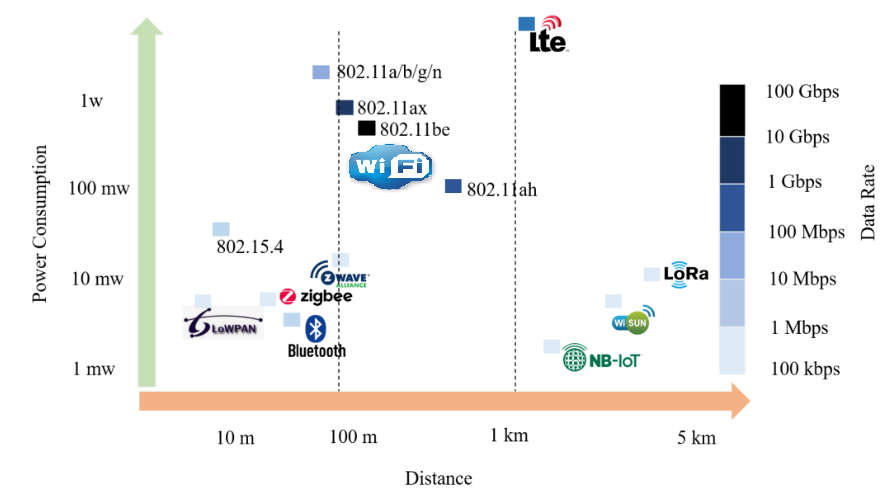
\includegraphics[scale=0.9]{images/PerformanceMap.png}
\caption{Power consumption, coverage distance, and data rate for the different protocols.}
\label{fig:x Performance MAP}
\end{figure}
The choice of wireless protocol depends on factors such as range, data rate, power consumption, latency, scalability, security, cost, deployment environment, and application requirements \cite{PerformanceMAP}. Each protocol is designed to address specific use cases, and selecting the right one involves evaluating these factors to meet the demands of your IoT deployment. After analysing all the parameters, requirements, and studying the LTE-M System Performance from \cite{LTE-M_Perform}, we have chosen NB-IoT protocol for our acquisition system.

\nomenclature{$IoT$}{Internet of Things}
\nomenclature{$LAN$}{Local Area Network}
\nomenclature{$BLE$}{Bluetooth Low Energy}
\nomenclature{$LoRaWAN$}{Long Range Wide Area Network}
\nomenclature{$NB-IoT$}{Narrowband IoT}
\nomenclature{$LTE-M$}{Long Term Evolution Machine Type Communication}
\nomenclature{$AES$}{Advanced Encryption Standard}
\nomenclature{$Wi-SUN$}{Internet of Things}
\nomenclature{$WiFi$}{Wireless Smart Utility Network}





\chapter{Hardware Implementation}\label{Hardware}

%\section{First and Second}
%\chapter{Hardware Implementation} 
\section{Block Diagram} 
Electrical data acquisition and supervision system refer to the process of collecting, monitoring, and analyzing electrical data from various sources to gain insights, detect anomalies, and ensure the proper functioning of our electrical systems. This can be achieved through the use of sensors, data acquisition systems, and monitoring platforms. The design block shown in figure \ref{fig:x System Block}, depicts a complete scenario of our project. 

\begin{figure}[htbp]
\centering
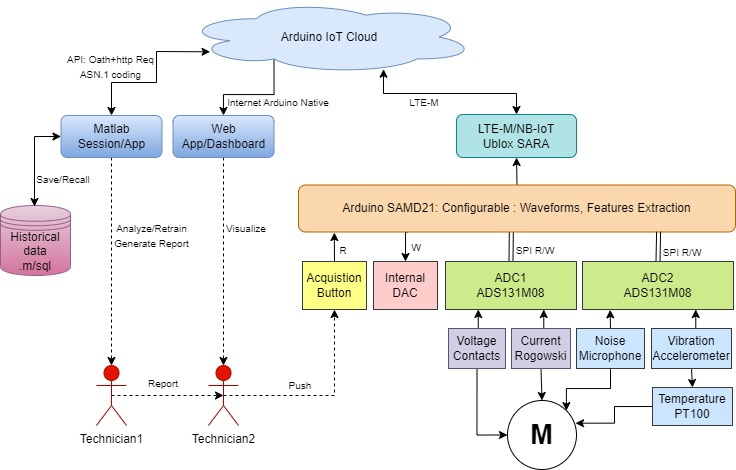
\includegraphics[scale=0.5]{images/Acqsys.jpg}
\caption{ADS131M08 based Acquisition System Block}
\label{fig:x System Block}
\end{figure}

From the figure above, we can observe that this acquisition system can be accessed both manually and via a Matlab session. For the manual option, Technician2 on-site pushes the button. Then, two ADS131M08 ADCs handle the analog data from voltage contacts, current Rogowski sensors, noise, and vibration. The Arduino SAMD21 ARM Cortex M0 processor collects these analog data through SPI communication and sends them to the Arduino IoT cloud using LTE-M. The analog data becomes visible in the cloud, and this acquisition can also be controlled from a push button designed in the cloud. Internal DAC generates analog waveforms for our calibration in house R\&D purpose.
Technician1 can analyze the sample data from the cloud using local Matlab web access. Reading from and writing to the cloud are possible through Matlab web access scripts. Technician1 can also write register values to ADCs via API oath and IoT protocol. For further feature extractions, the RMS calculation algorithm is generated using Simulink, and the resulting C codes can be integrated with the Arduino firmware. 

\section{Arduino MKR NB-IoT} 
In order to provide IoT (Internet of Things) capability combining Narrowband IoT (NB-IoT) and LTE CAT-M1 (LTE-M) communication technologies, Arduino created the Arduino MKR NB 1500, a specialized version of the Arduino MKR family. This gadget combines the capabilities of an Arduino microcontroller with a cellular network to provide cellular network connection to the internet. The pin configuration of an Arduino MKR 1500 has been shown in figure \ref{fig:x Arduino Pinout}. \par
\begin{figure}[htbp]
\centering
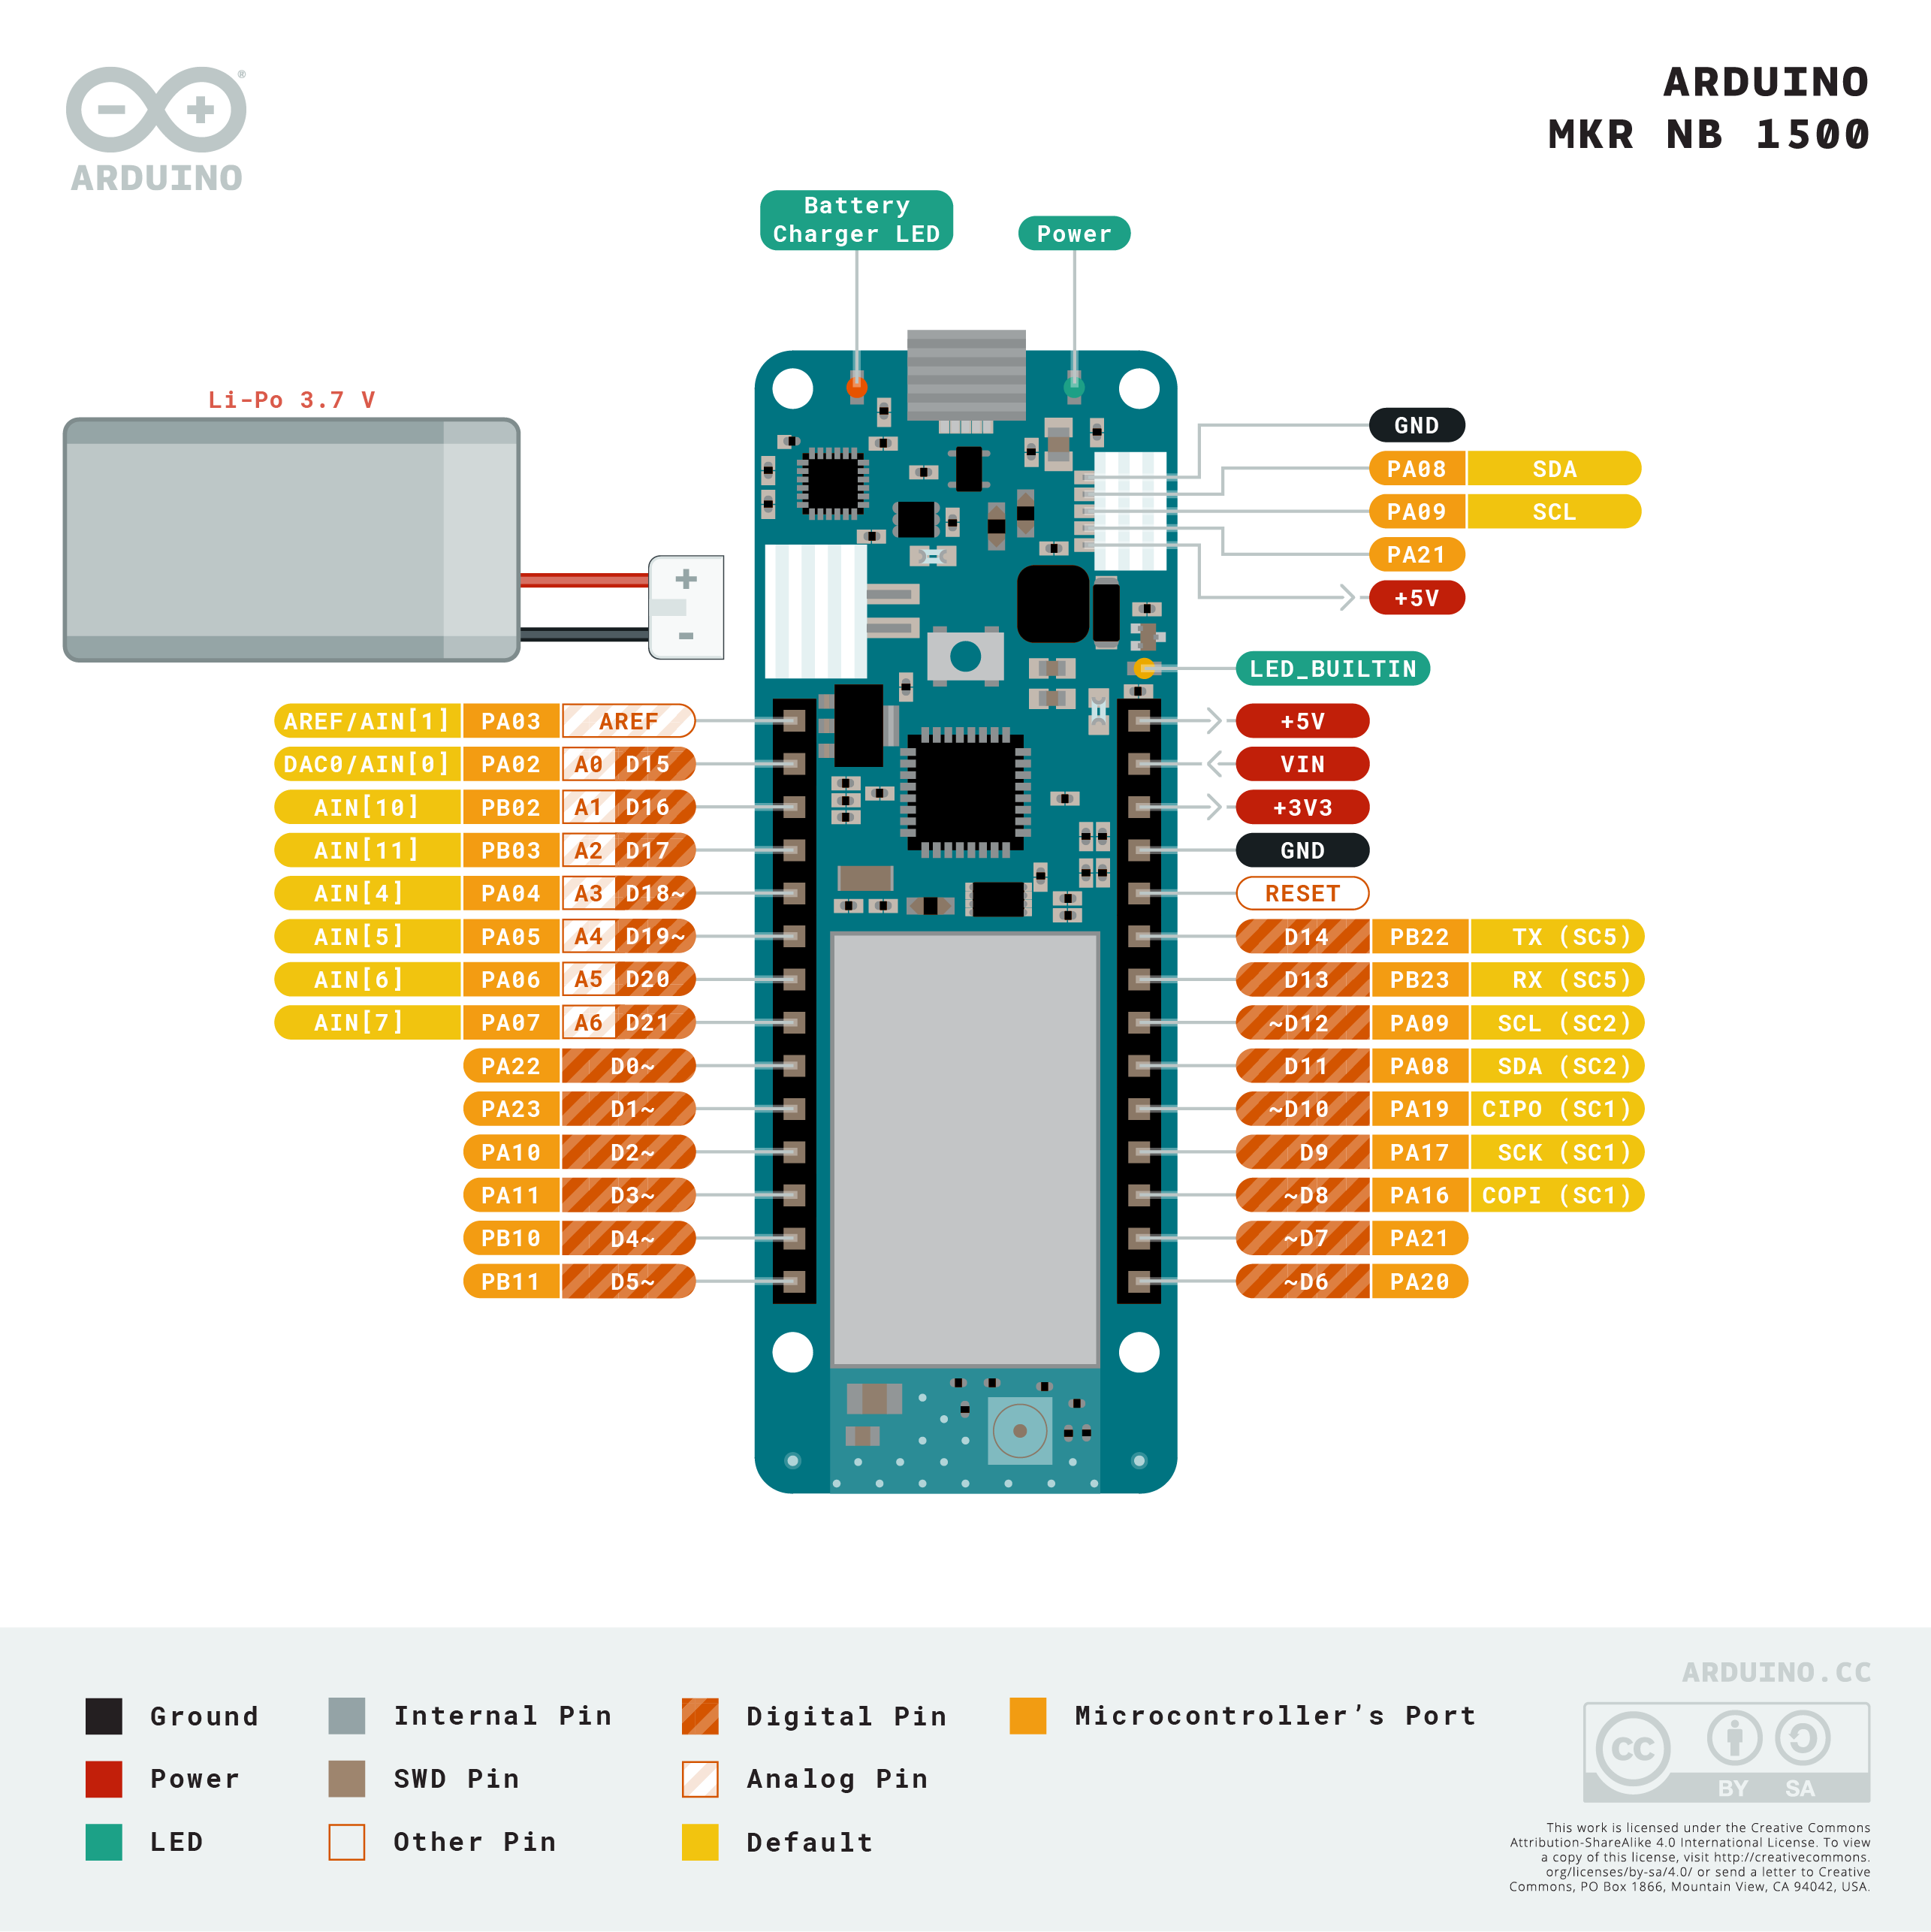
\includegraphics[scale=0.4]{images/Arduino MKR.png}
\caption{Pinout of Arduino MKR NB 1500}
\label{fig:x Arduino Pinout}
\end{figure}
We have selected this board for prototype because of the Key features listed below:\par
\textbf{Communication:} It facilitates communication via LTE CAT-M1 and NB-IoT networks. These are low-power wide-area networks created for Internet of Things (IoT) devices, offering effective and economical data transfer for a range of applications.

\par 
\textbf{Microcontroller:} An ARM Cortex-M0+ microcontroller, which provides computing power and I/O capabilities for communicating with sensors, actuators, and other peripheral devices, is installed on the board.

\par 
\textbf{Integrated SIM Slot:} With an integrated SIM card slot, the MKR NB 1500 makes it simple to connect to the cellular network without the use of additional modules.

\par 
\textbf{Power Management:}The board is designed for low-power operation, making it effective for battery-powered or other power-restricted applications.

\par 
\textbf{Form Factor:} The MKR series boards feature a tiny footprint and a compact form factor, making them ideal for projects with limited space.

\par 
\textbf{Compatibility:} A wide range of I/O pins on the board enable it to interact with a number of sensors, actuators, and other parts frequently used in IoT applications.


\section{ADS131M08 Delta-Sigma ADC} \label{ADS131M08}
Delta-sigma ADCs are commonly used for applications that require high-resolution and high-precision analog-to-digital conversion, such as industrial instrumentation, medical devices, and data acquisition systems. Texas Instruments produces the ADS131M08 analog-to-digital converter (ADC) integrated circuit. In a physical view its a 32 pin ADC shown in figure \ref{fig:x ADS131M08 Chip}. For applications that demand precise and dependable data conversion from analog to digital format, this high-precision, low-power, 24-bit ADC has been developed. All the technical details of this eight channel delta-sigma ADC are available in the Datasheet \cite{ADSDatasheet}. In this section we will discuss some keynote points which were required to configure this ADC.
\begin{figure}[htbp]
\centering
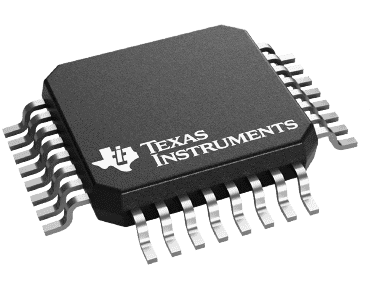
\includegraphics[scale=0.8]{images/ADS131M08 Chip.png}
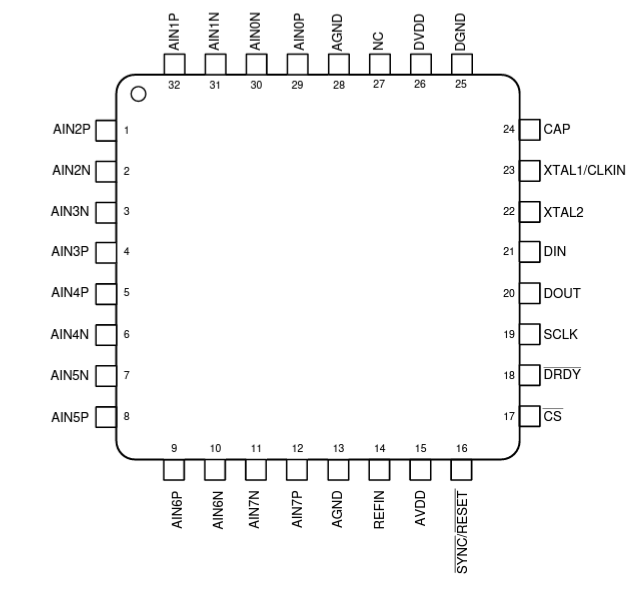
\includegraphics[scale=0.5]{images/pinoutADC.png}
\caption{ADS131M08 Pin  Configuration}
\label{fig:x ADS131M08 Chip}
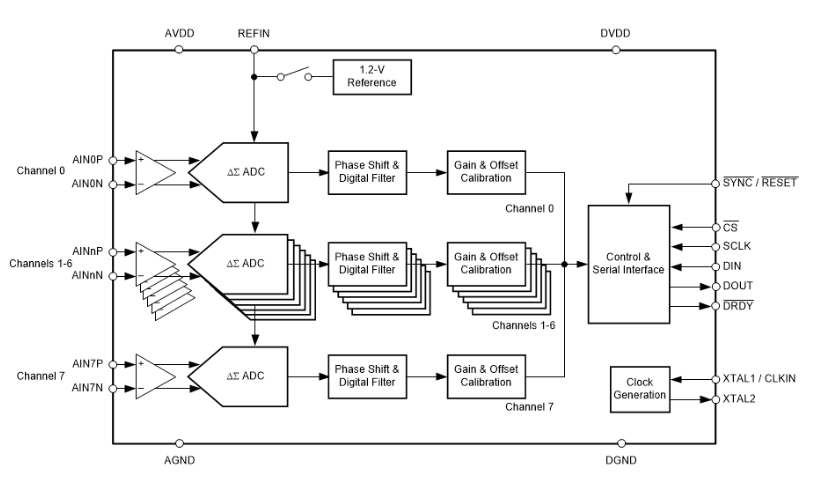
\includegraphics[scale=0.7]{images/Block ADC.png}
\caption{ADS131M08 functional Block}
\label{fig:x ADS131M08 Block}
\end{figure}
Sources for ADS131M08 must be both analog as well as digital. The AVDD-AGND analog source of power may function between 2.7 V and 3.6 V. Absolute input voltages can be as low as 1.3 V below AGND thanks to an incorporated negative charge pump, allowing single-ended power supplies to be used for measurements of input signals that fluctuate around ground. Both 1.8-V and 3.3-V sources are accepted by the digital power supply (DVDD - DGND). A PGA (programmable gain amplifier) with gains of up to 128 is a feature of the gadget. High input impedance is guaranteed at high PGA gain levels via an incorporated input precharge buffer active at gains larger than 4. An inbuilt 1.2-V reference provides the ADC with its reference voltage.Designers can choose between power consumption and ADC dynamic range using three power-scaling options. 
\vspace{1\baselineskip}\par 
The output of the modulators is demodulated by a digital decimation filter that is included into each channel of the ADS131M08. In high-resolution mode, the filter allows data rates of up to 32 kSPS per channel. A precise correction for the sensor phase responses is made possible by the ability to set the relative phase of the samples between channels. It is possible to configure offset and gain calibration registers to automatically correct output samples for detected offset and gain faults. The ADS131M08's functional block diagram in figure \ref{fig:x ADS131M08 Block} offers a thorough illustration of the device. A serial programming interface (SPI) compliant interface is used by the device for communication. The ADS131M08 is managed through a number of internal registers and SPI instructions. 
\vspace{1\baselineskip}\par 
\textbf{PGA:}  \par
 PGA refers to an electronic amplifier that allows the user to adjust its gain (amplification factor) according to their needs.The ADS131M08 has a built-in programmable gain amplifier (PGA) for each channel that offers gains of 1, 2, 4, 8, 16, 32, 64, and 128. The PGAGAINn bits for every channel in the GAIN1 register separately regulate the gains for the various channels. The differential full-scale input voltage range (FSR) of the ADC is scaled by changing the PGA gain. The link between FSR and gain is shown in equation \ref{eqn}. This Equation employs 1.2 V as the internal reference voltage as the scaling factor without taking into consideration gain error brought on the reference voltage tolerance.
\begin{align} \label{eqn}
    FSR = \pm 1.2 V / Gain
\end{align}
\textbf{Voltage Reference:}  \par
An internal and an external reference are the two voltage-reference choices available for the ADS131M08. The reference for the ADC is supplied by the internal reference using a low-drift band-gap voltage. The differential input voltage can range from -1.2 V to 1.2 V since the internal reference has a nominal value of 1.2 V. 
\vspace{1\baselineskip}\par 
\textbf{Clocking and Power Mode:}  \par
A crystal must be attached between the XTAL1/CLKIN and XTAL2 pins in order for the onboard oscillator to create the master clock whether internally or externally through the CLKIN pin.  The serial data clock (SCLK) must be synchronized with the modulator sampling clock for best performance.Since the master clock is the source of the modulator sampling clock, the master clock and SCLK must be in synchronization.  Therefore, for optimum performance, ensure that data retrieval is synchronized to the clock signal at CLKIN and supply a master clock to CLKIN.The device may be set up in any of the all three power modes: high-resolution (HR), low-power (LP), or very low-power (VLP), thanks to the PWR[1:0] bits in the CLOCK register. The internal bias currents are scaled to reach the desired power levels by changing the PWR[1:0] bits.

 
\vspace{1\baselineskip}\par 
\textbf{Delta-Sigma Modulator:}  \par
The conventional input voltage is converted to a one's density modulated digital bit-stream by the ADS131M08 using a delta-sigma ($\Delta\Sigma$) modulator. The ($\Delta\Sigma$) modulation circuit oversamples the supplied voltage at a frequency that is several times higher than its final data rate. The ADS131M08's modulation frequency, $f_{MOD}$, is equivalent to halves of the master clock frequency, or $f_{MOD} = f_{CLKIN} / 2$

\vspace{1\baselineskip}\par 
\textbf{Digital Filter:}  \par
The bitstream from the $\Delta\Sigma$ modulation is fed into the digital filter. The digital filter reduces the out-of-band noise caused by quantization of the modulator and is a linear phase, finite impulse response (FIR), and low-pass sinc-type filtering. By averaging, the digital filter demodulates the $\Delta\Sigma$ modulator's outputs. To decrease the rate at which data exit the modulation unit ($f_{MOD}$) and reach the output data stream ($f_{DATA}$), the data flowing through the filter is downsampled and shredded. Equation \ref{OSReqn} defines the decimation factor, which is also known as the oversampling ratio (OSR).
\begin{align} \label{OSReqn}
    OSR = f_{MOD}/f_{DATA}
\end{align}
The OSR[2:0] entries in the CLOCK register control the OSR and modify it. The ADS131M08 has OSR options that enable various data rate configurations for any specific master clock frequency. For the specified notional CLKIN frequencies, Table \ref{tab:OSR} gives the OSR parameters and their respective output data rates. There are three different types of power mode of this ADC. We have configured it to the Very Low Power (VLP) mode by providing 2.048 MHz clock frequency, and output data rate was 1 ksps.
\begin{table}[htbp]
  \centering
     \caption{OSR Settings and Data Rates}
    \label{tab:OSR}
  \begin{tabular}{|c|c|c|c|c|}
    \hline
    \multicolumn{1}{|c|}{\textbf{Power Mode}} & \multicolumn{1}{|c|}{\textbf{Clock}} & \multicolumn{1}{|c|}{\textbf{$f_{MOD}$}} & \multicolumn{1}{c|}{\textbf{OSR}} & \multicolumn{1}{c|}{\textbf{O/P Data}} \\
    \hline
    \multirow{8}{*}{VLP} & \multirow{8}{*}{2.048 MHz} & \multirow{8}{*}{1.024 MHz} & 128 & 8 KSPS \\
    & & & 256 & 4 KSPS \\
    & & & 512 & 2 KSPS \\
    & & & 1024 & 1 KSPS \\
    & & & 2048  & 500 SPS \\
    & & & 4096 & 250 SPS \\
    & & & 8192 & 125 SPS \\
    & & & 16384 & 62.5 SPS \\
    \hline
  \end{tabular}

\end{table}

\section{Schematic Diagram} 
The schematic shown in figure \ref{fig:x Schematic} has been designed in KiCad software. There are several portions of this schematic which has been listed below:
\begin{figure}[htbp]
\centering
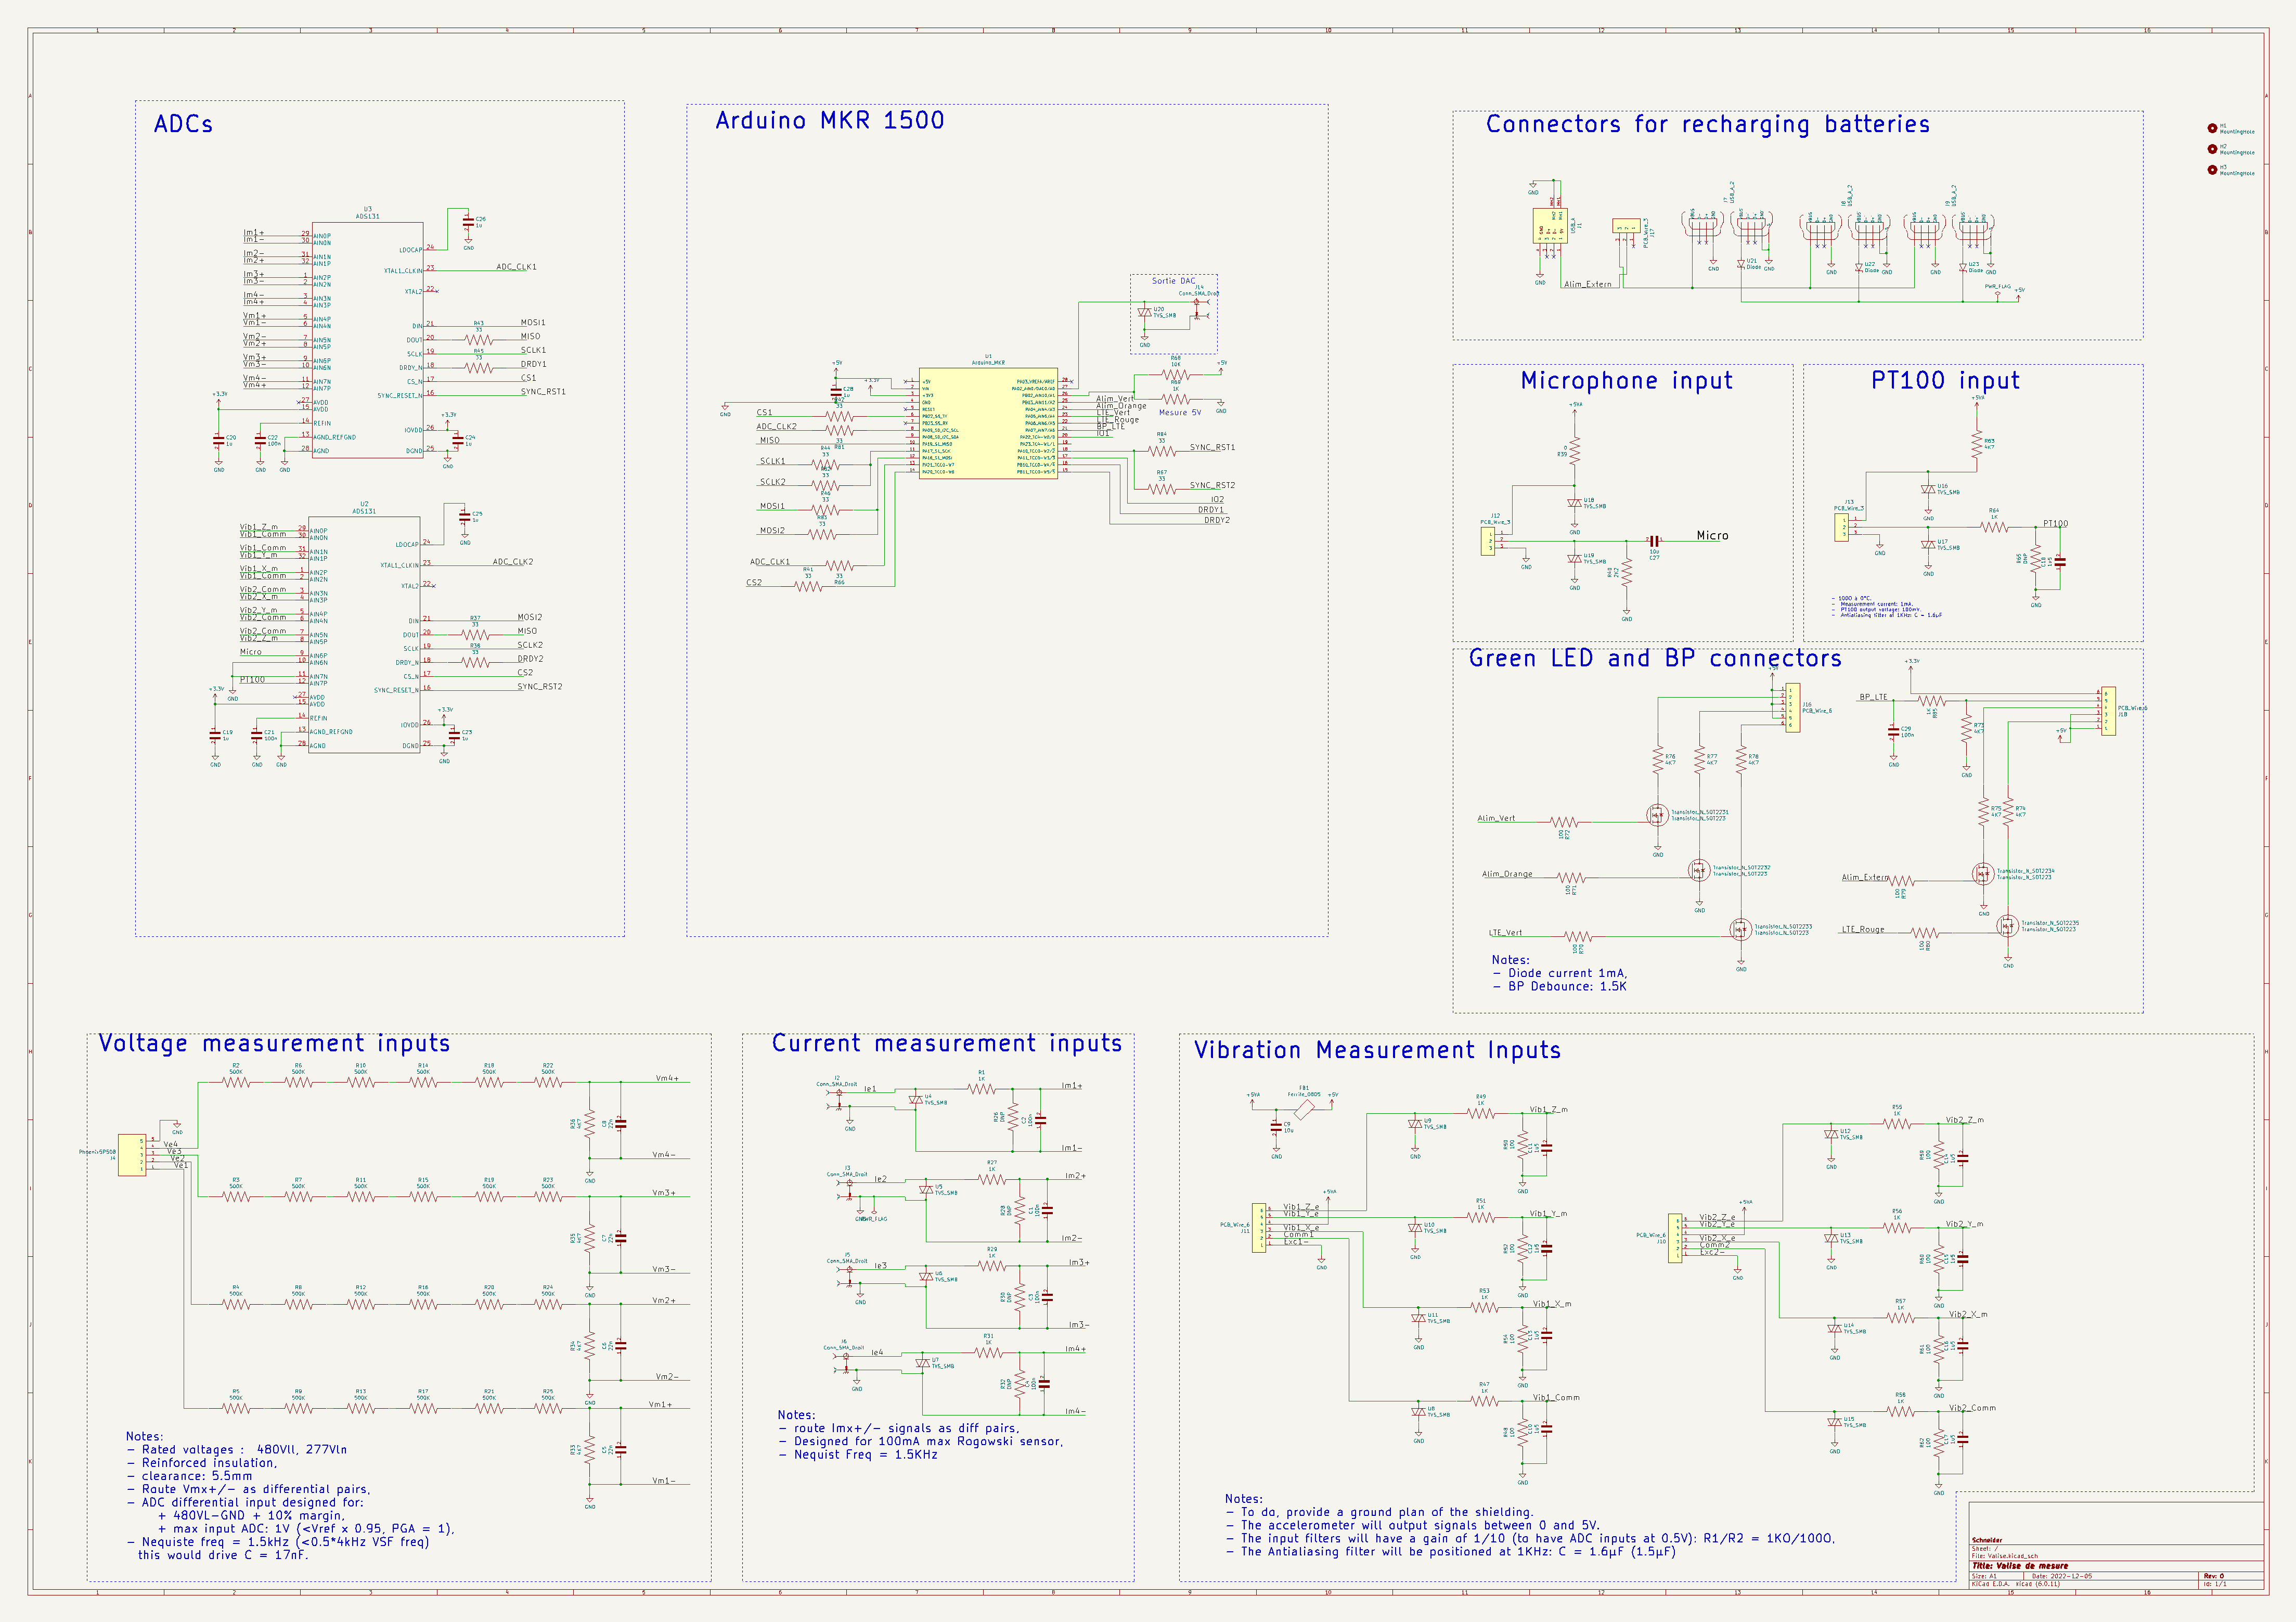
\includegraphics[scale=0.18]{images/Schematic.png}
\caption{Schematic Diagram}
\label{fig:x Schematic}
\end{figure}

\begin{itemize}
\begin{multicols}{2}
  \item Arduino MKR 1500
  \item Two ADCs
    \item PT100 Input
  \item Green LED \& Push Button 
  \item Microphone Input
  \item Voltage Measurement Input
  \item Current Measurement Input
  \item Vibration Measurement Input
   \item Connection for Recharging Batteries
\end{multicols}
\end{itemize}







\section{Printed Circuit Board Assembly} 

The PCBA process is a crucial stage in electronic manufacturing and requires careful attention to detail and quality control to ensure reliable and functional electronic products. Printed Circuit Board Assembly (PCBA) refers to the process of attaching electronic components onto a printed circuit board (PCB) to create a functional electronic circuit.This PCBA process typically involves the following steps:
\par
\textbf{PCB Fabrication: } 
 First, the bare PCB is manufactured by etching copper traces onto an insulating substrate according to the design specifications. The PCB layout is designed using specialized software and contains the necessary traces, pads, and vias to connect the components. We have designed our PCB in KiCad software shown in figure \ref{fig:x PCB design}, and fabricated it from a third party PCB manufacturer.\par
\begin{figure}[htbp]
\centering
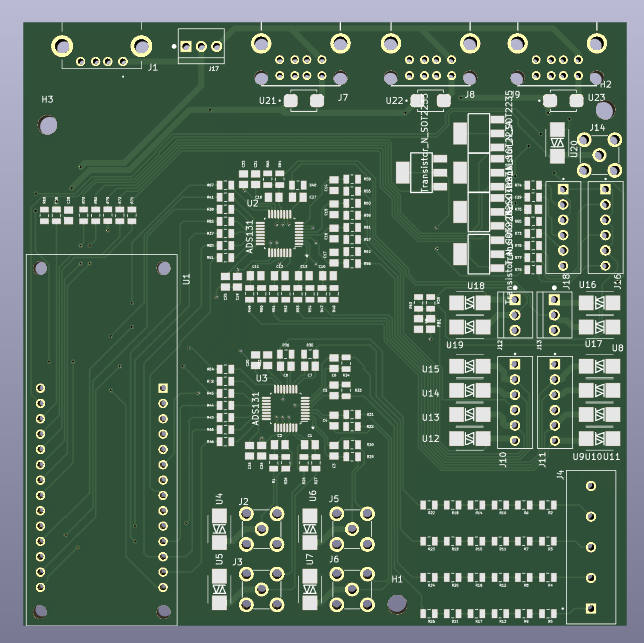
\includegraphics[scale=0.55]{images/Valise.png}
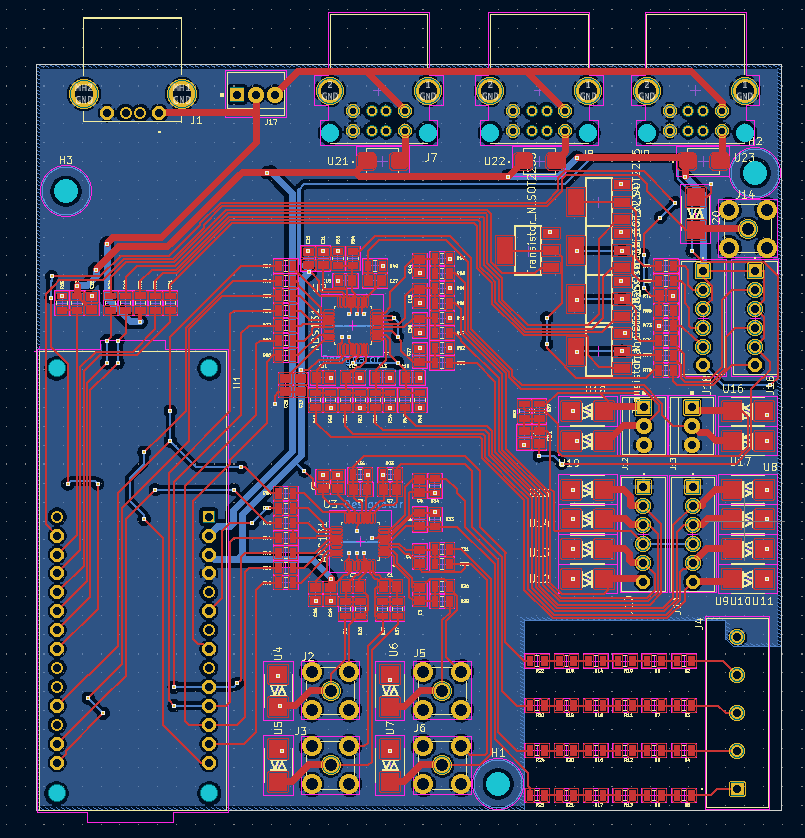
\includegraphics[scale=0.42]{images/PCB Valise.png}
\caption{PCB design of Acquisition System}
\label{fig:x PCB design}
\end{figure}

\textbf{Component Placement:}  
Once the PCB is ready, the electronic components (such as resistors, capacitors, integrated circuits, connectors, etc.) are placed onto the board in their designated locations. There are two main methods for component placement:
\par
\textbf{a. Manual Assembly:}  
 Smaller scale productions may involve manual placement of components. Skilled technicians use pick-and-place machines or soldering irons to carefully position each component.In Schneider's Lab we have implemented our board through manual assembly. Majority of the components on our board were SMD, including the ADC, which made this task quite challenging to overcome precisely.
\par
\textbf{b. Automated Assembly:}  
 For larger-scale production, robotic pick-and-place machines are used to automate the component placement process. The machine picks components from reels or trays and accurately places them onto the PCB based on the design data. In the future, we may consider employing this technique for mass production.
\par
\textbf{Soldering: }  
After the components are placed, they need to be permanently attached to the PCB. Soldering is the most common method for creating these connections. Weller WX 2021 SMD soldering station has been used for the soldering of our PCB.
\par
\begin{figure}[htbp]
\centering
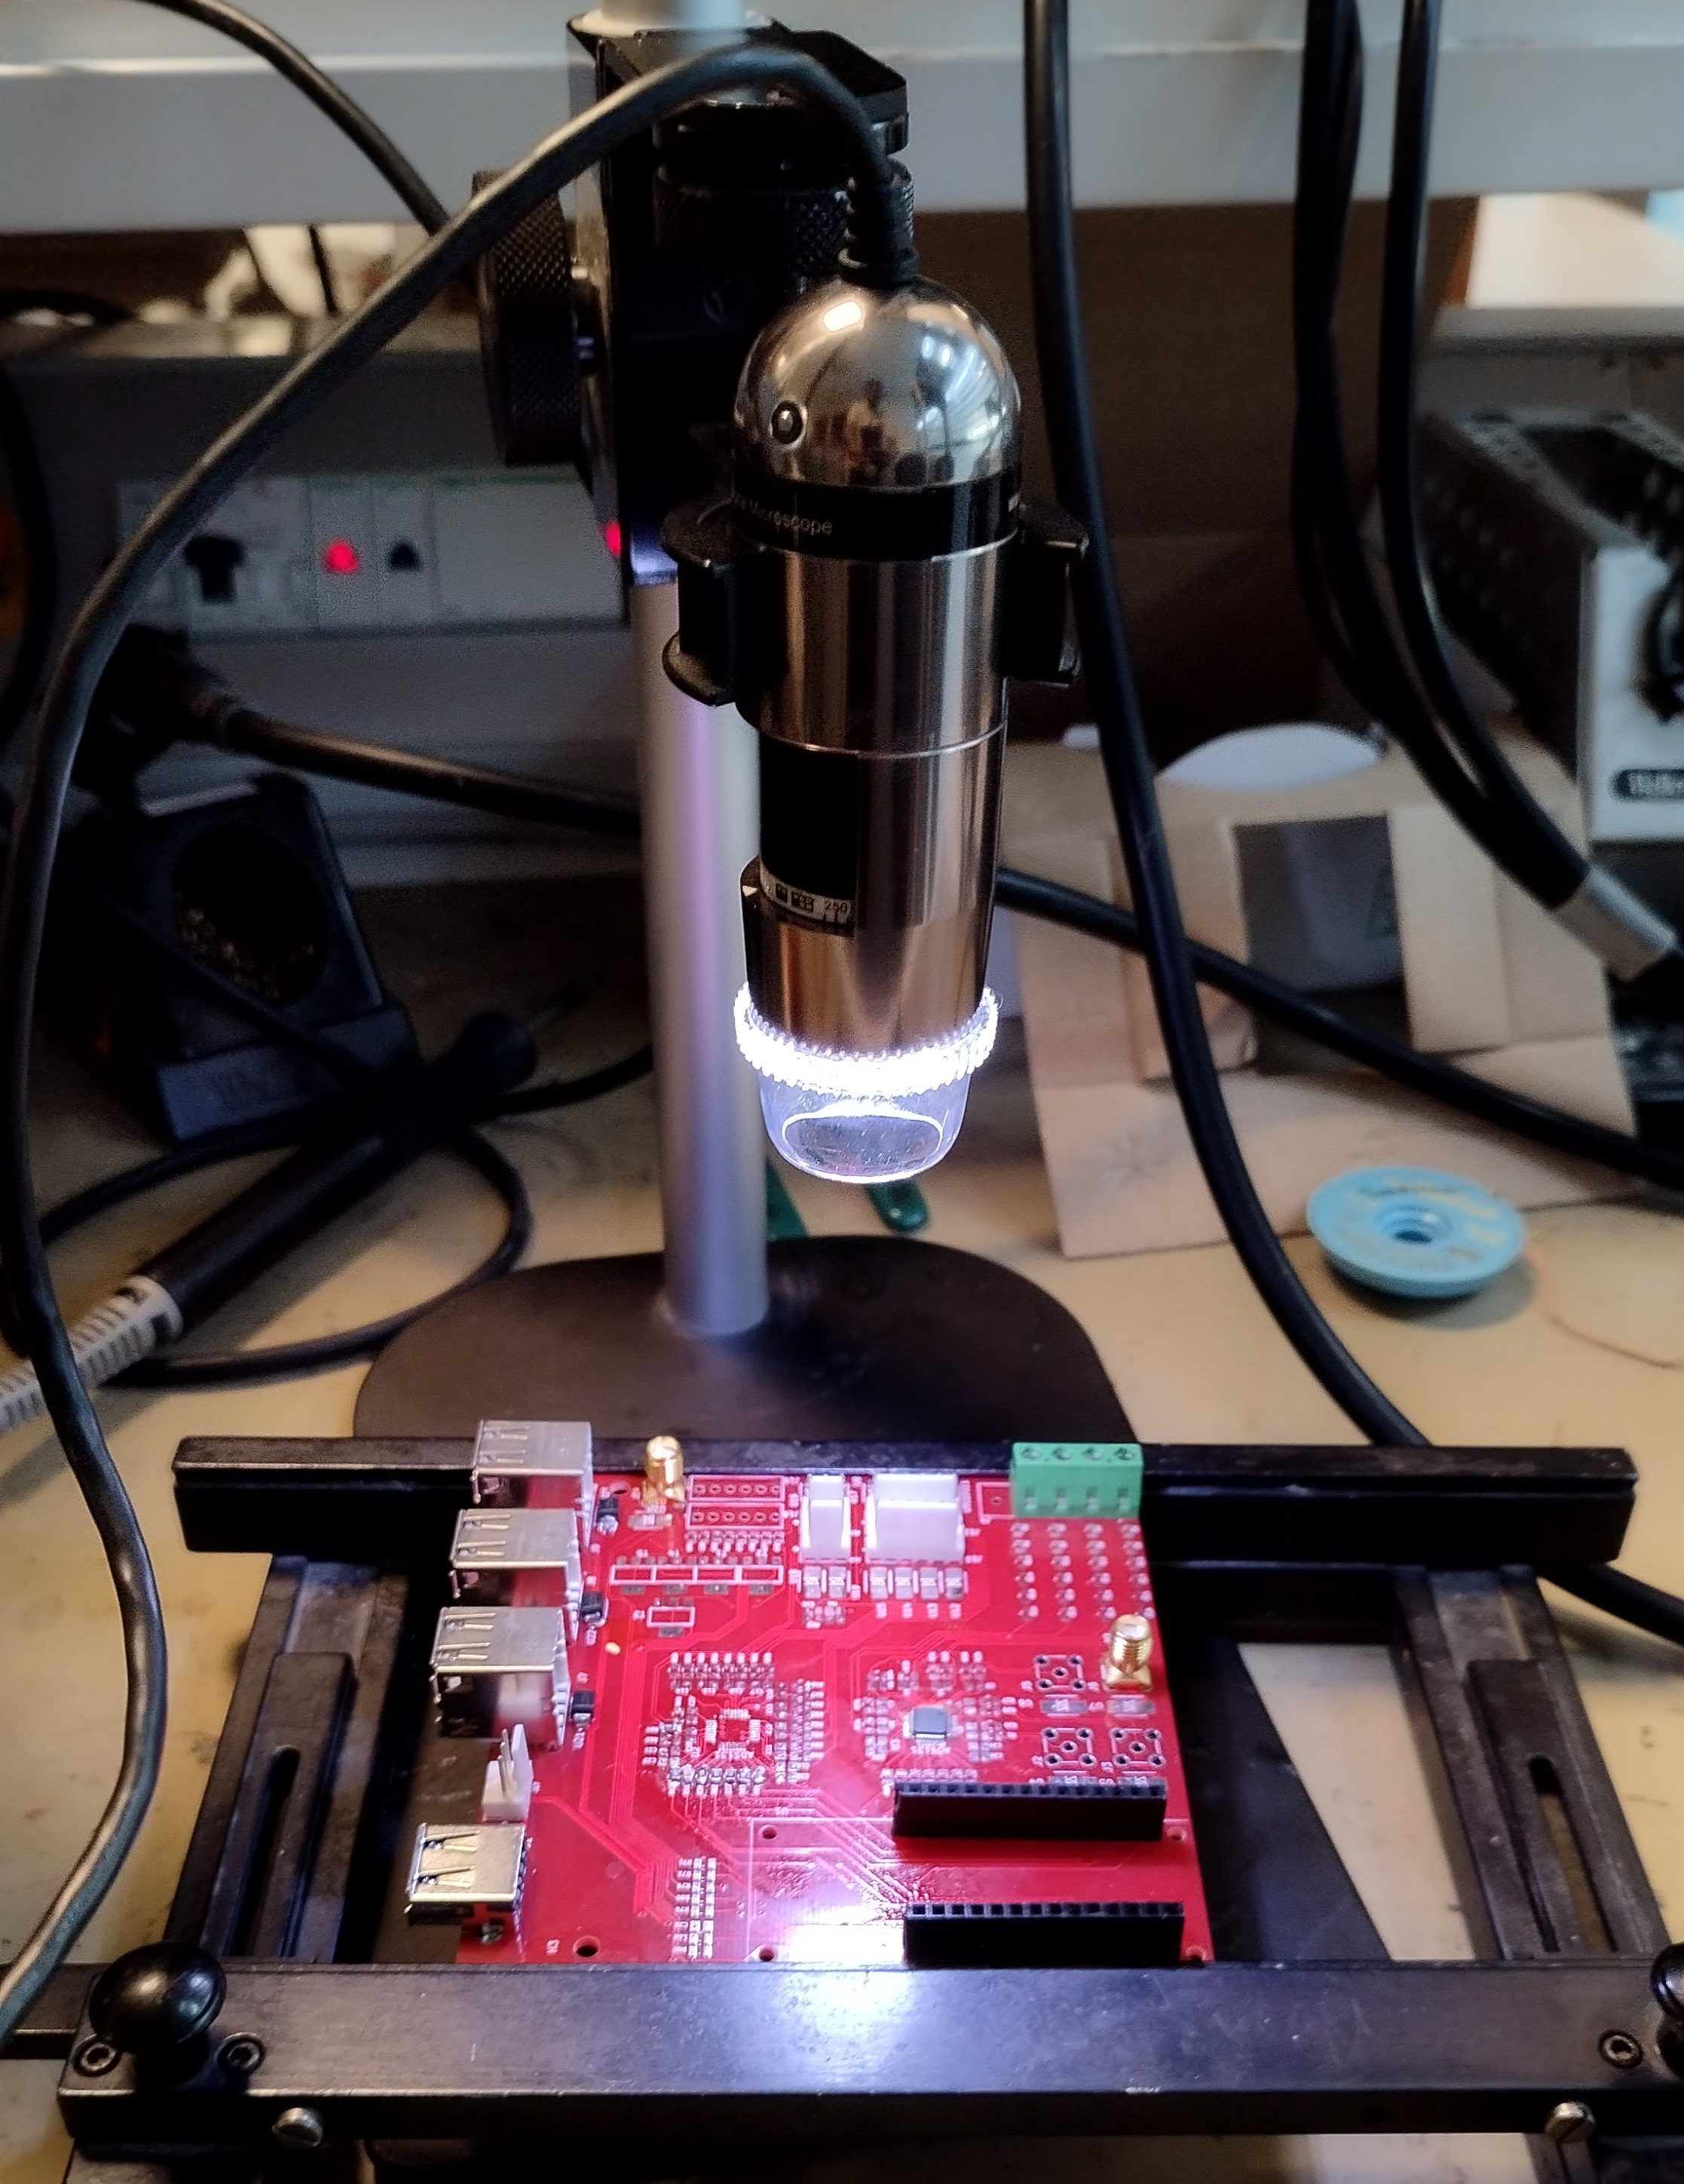
\includegraphics[scale=0.063]{images/Microscope.jpg}
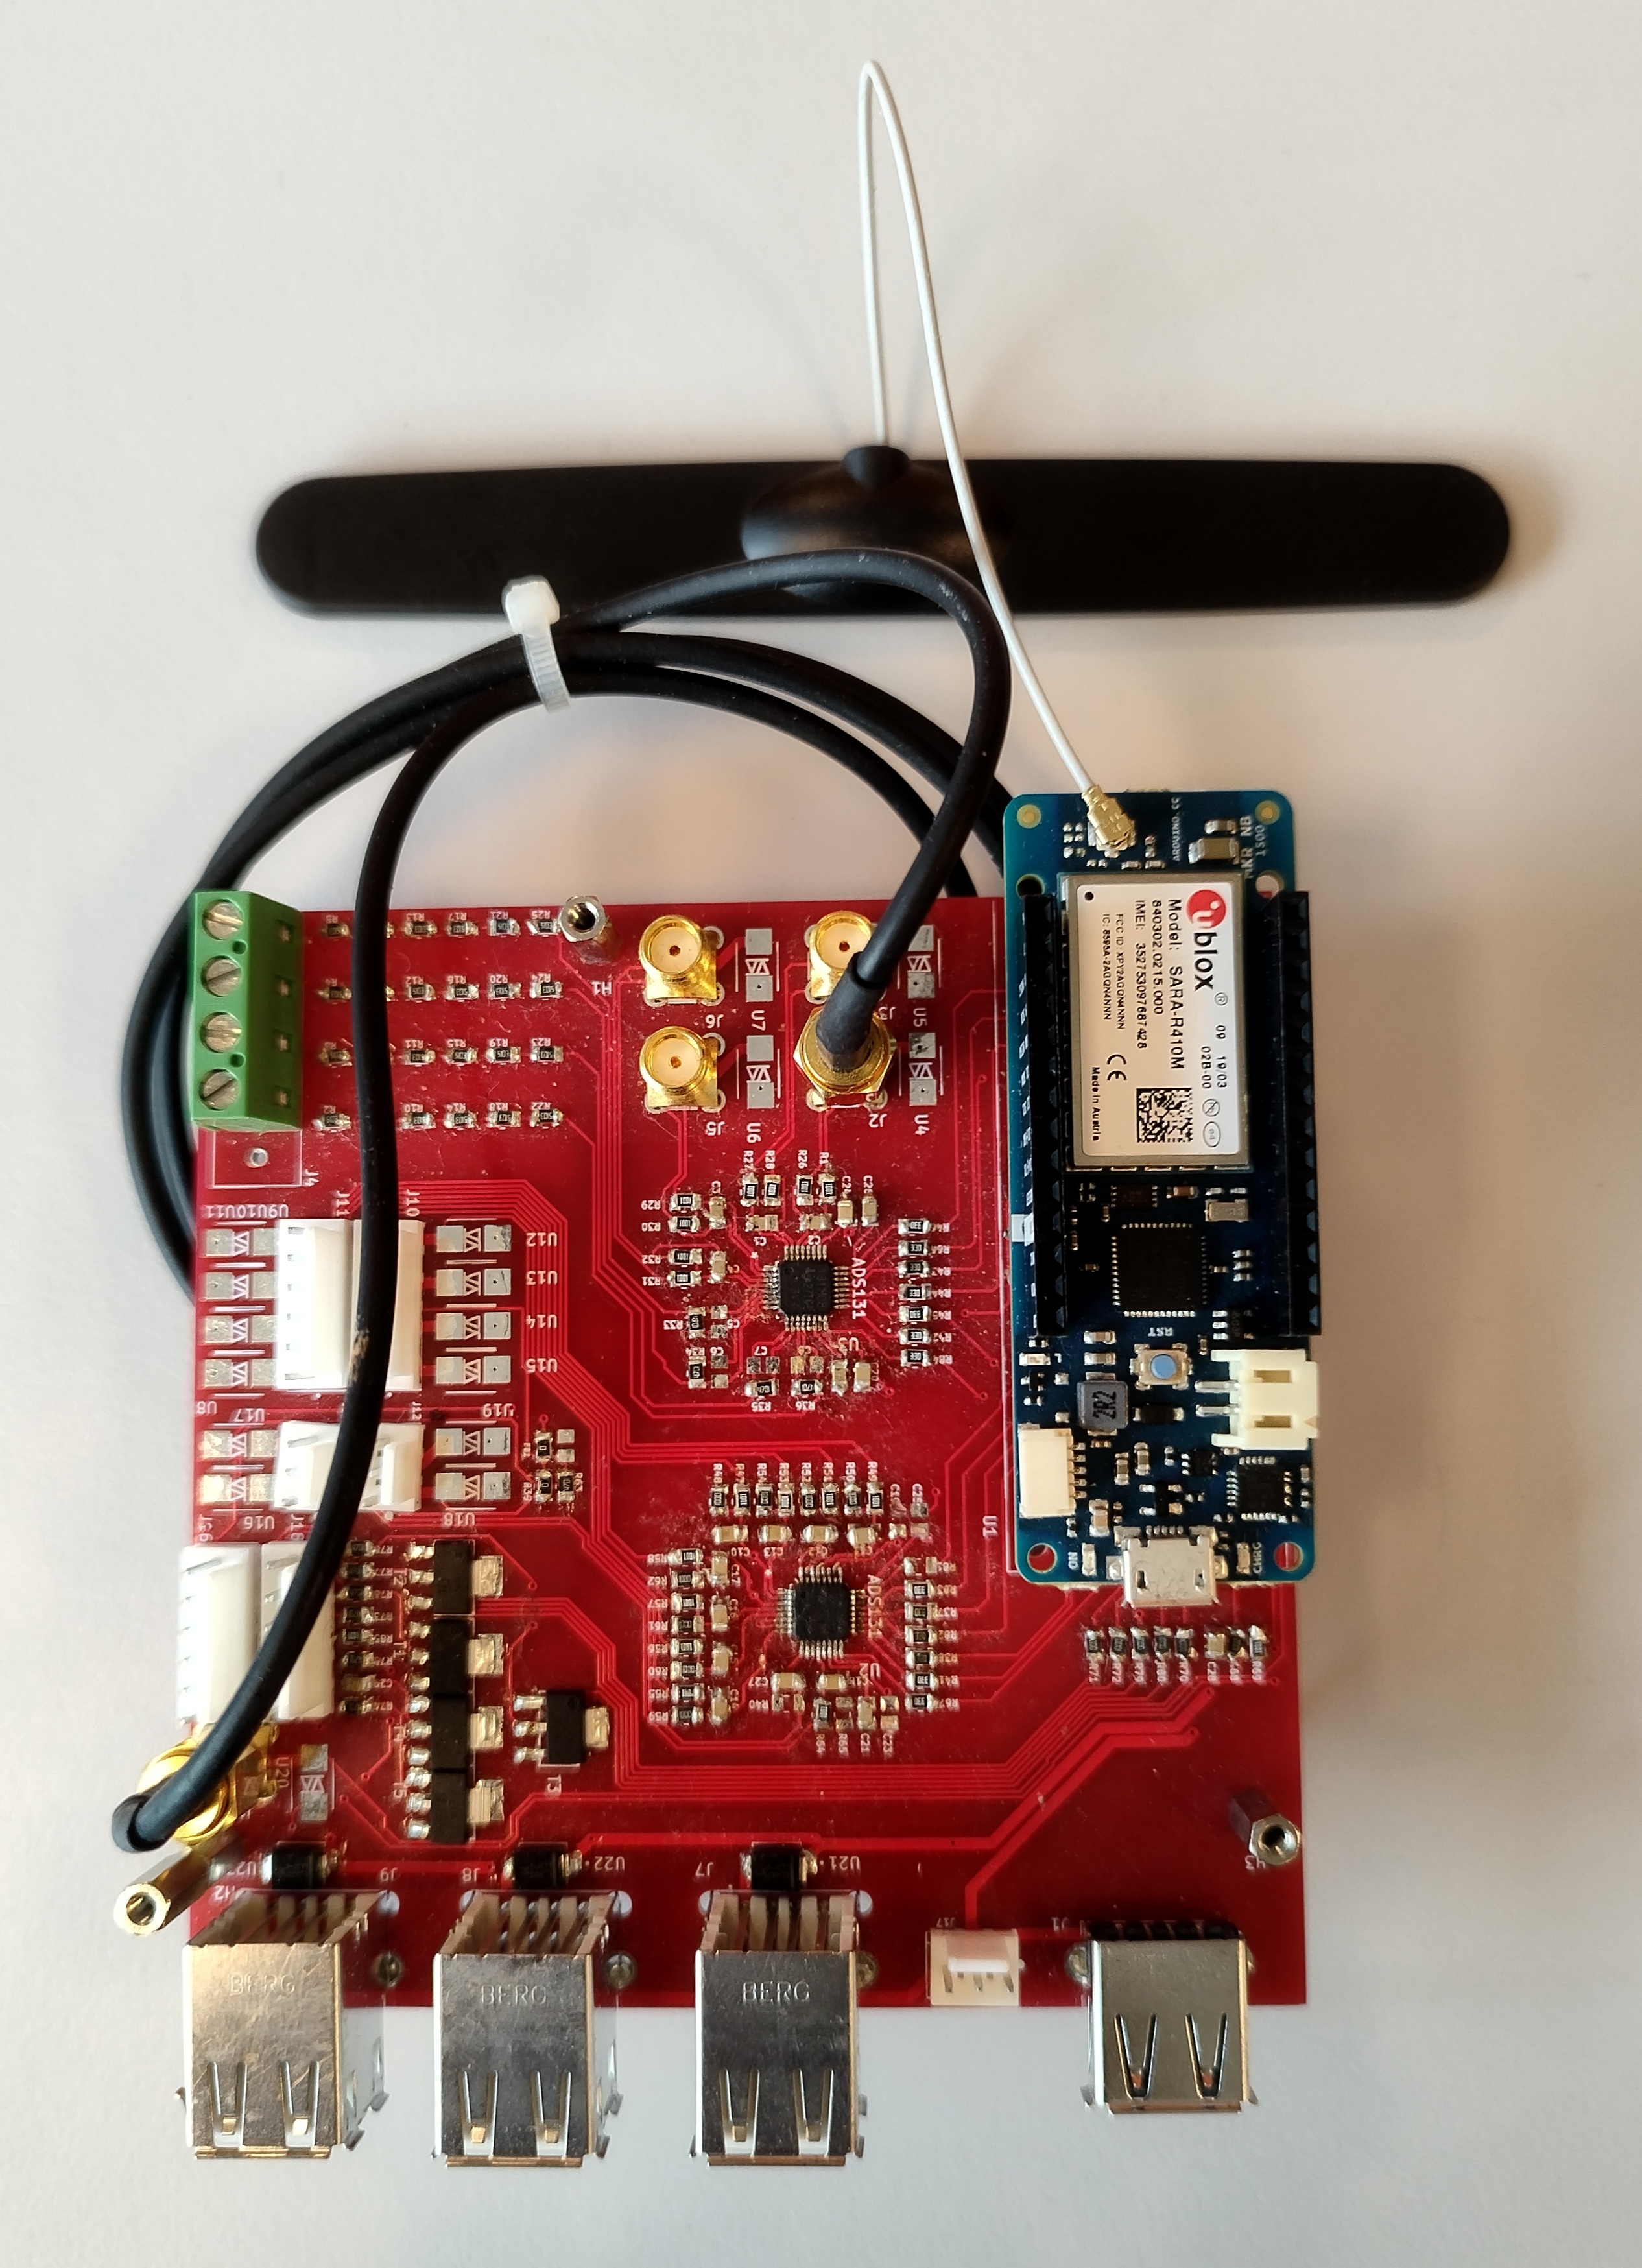
\includegraphics[scale=0.0525]{images/Board.jpg}
\caption{PCB Inspection and Implemented Board}
\label{fig:x Implemented Board}
\end{figure}
\textbf{Inspection and Testing:}  
 After soldering, the assembled PCBs undergo inspection to detect and correct any manufacturing defects such as solder bridges, missing components, or incorrect placements. Automated optical inspection (AOI) and X-ray machines are commonly used for this purpose. We have used Dino-Lite Edge AM73115MTF USB microscope for the inspection purpose shown in figure \ref{fig:x Implemented Board}. The final ready-to-run acquisition board also has been shown in the right figure.
\par

\nomenclature{$API$}{Application Programming Interface}
\nomenclature{$RMS$}{Root Mean Square}
\nomenclature{$PGA$}{Programmable Gain Amplifier}
\nomenclature{$KSPS$}{Kilo Samples Per Second}
\nomenclature{$SPI$}{Serial Peripheral Interface}
\nomenclature{$XTAL$}{Crystal}
\nomenclature{$PCB$}{Printed Circuit Board}
\nomenclature{$LP$}{Low Power}
\nomenclature{$VLP$}{Very Low Power}

\chapter{Software Implementation}\label{Software}

%\section{Software Implementation}
\section{Software Architecture} 
The crucial part of this project was to develop the firmware of the system. We choose the PlatformIO ecosystem and integrated it into Visual Studio Code. PlatformIO is an open-source ecosystem for IoT development that provides an IDE for various microcontroller platforms. 
\begin{figure}[htbp]
\centering
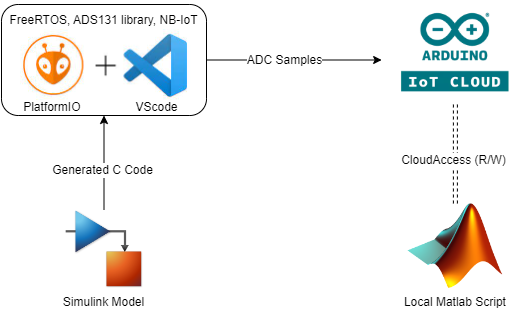
\includegraphics[scale=0.5]{images/Software Architecture.png}
\caption{Software Architecture}
\label{fig:x Software Architecture}
\end{figure}
The figure \ref{fig:x Software Architecture} depicts the whole software development process.We developed the ADC library within the firmware, along with configuring NB-IoT configuration within the Real-Time Operating System FreeRTOS. The ADC samples are transmitted to the Arduino Cloud, where the data can be read and written through a local Matlab script. Moreover, a Simulink model was created for computing RMS. This feature extraction algorithm generates C code that updates the firmware, enabling the calculation of subsequent samples within a synchronous function. Any kind of anomaly in electrical parameters are instantly available in cloud server.
\section{ADC Configuration \& Calibration} 
\subsection{Programming ADC} 
\textbf{Chip Select($\overline{CS}$):} The component is chosen to communicate by the active low input signal on the $\overline{CS}$ pin. When $\overline{CS}$ is set high, the device rejects all communication and DOUT has a high impedance. To assure excellent communication, we need to keep $\overline{CS}$ Low for the entire length of a communication period. Each time $\overline{CS}$ is taken high, the interface is reset. \par

\textbf{Serial Data Clock (SCLK):} The interface's serial clocking is provided through the input known as SCLK. The data that is input on DIN is latching onto the falling edge of SCLK, whereas the data output upon the DOUT pin transitions on the rising edge of SCLK. Our clock was tuned to 2.195MHz shown in figure \ref{fig:x Clock Generation}. \par
\begin{figure}[htbp]
\centering
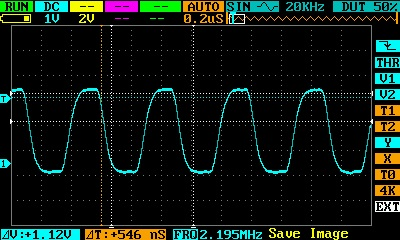
\includegraphics[scale=0.6]{images/2.195MHz.jpg}
\caption{Clock Generation for ADC}
\label{fig:x Clock Generation}
\end{figure}

\textbf{Serial Data Input (DIN):} Serial data entry for the device is performed employing the DIN pin. The device shifts a serial command in while the $\overline{CS}$ pin is low, via the DIN pin, for every SCLK falling edge. \par

\textbf{Serial Data Output (DOUT):} The device's DOUT pin acts as the serial data outputting pin. Whenever the $\overline{CS}$ pin is low, the device shifts out command responds and ADC data from conversion serially over each rising SCLK edge. Once $\overline{CS}$ is high, this pin approaches a condition of high impedance. \par

\textbf{Data Ready ($\overline{DRDY}$):} The $\overline{DRDY}$ pin represents an active low-powered output that signals while new conversions data are available in converting mode or whenever current detection criteria are satisfied in current-detect mode. \par

\textbf{SPI Communication:} Serial Peripheral Interface, is a widely used synchronous serial communication protocol that allows communication between microcontrollers, sensors, and other peripheral devices. The SPI communication typically involves one master device and one or more slave devices. The master device controls the communication by generating a clock signal (SCLK) and selecting the slave devices with a chip select signal ($\overline{CS}$). Each slave device has a unique $\overline{CS}$ pin to distinguish it from others on the bus.  \par
\vspace{1\baselineskip}\par 
Communication via the SPI with the ADS131M08 is carried out in frames. Each SPI signaling frame consists of multiple words. The word size may be set to 16 bits, 24 bits, or 32 bits through modifying the WLENGTH[1:0] bits in the MODE register.
\begin{figure}[htbp]
\centering
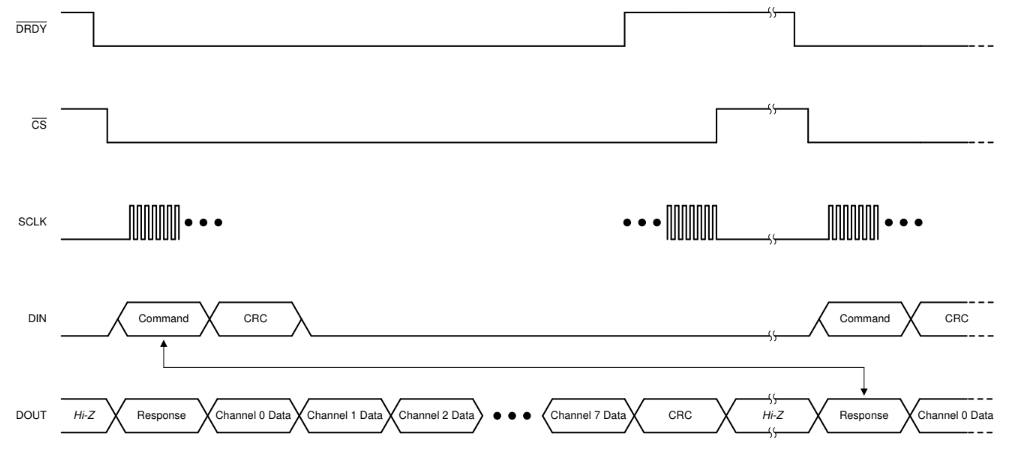
\includegraphics[scale=0.6]{images/Communication_Frame.png}
\caption{SPI Communication Frame}
\label{fig:x Communication Frame}
\end{figure}
The communication frame shown in figure \ref{fig:x Communication Frame} is full duplex, which means it can broadcast data on DOUT while receive data on DIN at the same time. The host's DIN input frames always starts with a single command. The answer to the command that was typed on the prior input frame is always the first word on the output frames that the system streams on DOUT. The amount of words in a command is determined by the command. A frame typically contains ten words for most instructions. The host supplies the command, the command CRC if inputs CRC is enabled, or one word of zeros if input CRC is disabled, and eight further words of zeroes on DIN. On DOUT, the unit concurrently produces the prior frames command's answer, eight words of ADC data denoting the eight ADC channels, and a CRC word.


\subsection{Setting Registers} 
\textbf{Register Map:} There are total 51 registers in ADS131M08. The details of each register's bit fields and their specific functions can be found in the device's datasheet \cite{ADSDatasheet}. Here we have presented all 51 registers name and address in Table \ref{tab:Register Map}. \par
\begin{table}[htbp]
  \centering
        \caption{Register Map of ADS131M08}
  \label{tab:Register Map}
  \adjustbox{width=1\textwidth, height=0.18\textheight}{
    \begin{tabular}{*{6}{|c}|}
      \hline
      \textbf{Address} & \textbf{Register} & \textbf{Address} & \textbf{Register} & \textbf{Address} & \textbf{Register} \\
      \hline
      00h   & ID   & 11h   & CH1\_GCAL\_MSB   & 22h   & CH5\_CFG  \\
      01h   & STATUS   & 12h   & CH1\_GCAL\_LSB & 23h   & CH5\_OCAL\_MSB    \\
      02h   & MODE   & 13h   & CH2\_CFG   & 24h   & CH5\_OCAL\_LSB   \\
      03h   & CLOCK   & 14h   & CH2\_OCAL\_MSB   & 25h   & CH5\_GCAL\_MSB    \\
      04h   & GAIN1   & 15h  & CH2\_OCAL\_LSB   & 26h   & CH5\_GCAL\_LSB   \\
      05h  & GAIN2   & 16h   & CH2\_GCAL\_MSB   & 27h   & CH6\_CFG    \\
      06h   & CFG   & 17h   & CH2\_GCAL\_LSB   & 28h   & CH6\_OCAL\_MSB     \\
      07h  & THRSHLD\_MSB   & 18h  & CH3\_CFG  & 29h   & CH6\_OCAL\_LSB \\
      08h   & THRSHLD\_LSB   & 19h   & CH3\_OCAL\_MSB   & 2Ah   & CH6\_GCAL\_MSB  \\
      09h   & CH0\_CFG   & 1Ah  & CH3\_OCAL\_LSB   & 2Bh   & CH6\_GCAL\_LSB   \\
      0Ah   & CH0\_OCAL\_MSB   & 1Bh   & CH3\_GCAL\_MSB  & 2Ch   & CH7\_CFG  \\
      0Bh   & CH0\_OCAL\_LSB   & 1Ch   & CH3\_GCAL\_LSB   & 2Dh   & CH7\_OCAL\_MSB  \\
      0Ch   & CH0\_GCAL\_MSB  & 1Dh   & CH4\_CFG  & 2Eh   & CH7\_OCAL\_LSB  \\
      0Dh   & CH0\_GCAL\_LSB   & 1Eh  & CH4\_OCAL\_MSB   & 2Fh   & CH7\_GCAL\_MSB \\
      0Eh   & CH1\_CFG   & 1Fh   & CH4\_OCAL\_LSB   & 30h   & CH7\_GCAL\_LSB   \\
      0Fh   & CH1\_OCAL\_MSB   & 20h   & CH4\_GCAL\_MSB   & 3Eh   & REGMAP\_CRC  \\
      10h   & CH1\_OCAL\_LSB  & 21h   & CH4\_GCAL\_LSB   & 3Fh   & RESERVED   \\
      % Add more rows here with additional elements...
      \hline
    \end{tabular}

  }

\end{table}

\subsection{Reading Registers} 
Configuring the registers of the ADS131M08 entails defining several parameters that dictate the ADC's behavior and functionality. The ADS131M08 offers multiple interface modes including SPI, QSPI, and parallel interface. In our case, we have opted for SPI communication to facilitate both data reading and writing.Then we have configured the power mode, input ranges, PGA, sampling rate and filter settings in the CONFIG (CFG) register. Additionally, a register tables of value and address also has been developed for in future R/W operation. The table \ref{tab:CLOCK Register} illustrates the process of reading the CLOCK register, which designates 16 bits for distinct functions. Among these, Bit 0 and 1 are designated for PWR, Bits 2-4 for OSR settings, Bits 5-7 are RESERVED, and the range from Bit 8 to 15 corresponds to eight distinct channels that enable specific functions. 
\begin{table}[htbp]
  \centering
  \caption{CLOCK Register Setting}
  \label{tab:CLOCK Register}
  \adjustbox{width=1\textwidth, height=0.04\textheight}{
  \begin{tabular}{|c|c|c|c|c|c|c|c|c|c|c|}
    \hline
    \multirow{2}{*}{\textbf{Address}} & 
    \multirow{2}{*}{\textbf{Register}} & 
    \multirow{2}{*}{\textbf{Reset}} & \textbf{BIT 15} & \textbf{BIT 14} & \textbf{BIT 13} & \textbf{BIT 12} & \textbf{BIT 11} & \textbf{BIT 10} & \textbf{BIT 9} & \textbf{BIT 8} \\
    \cline{4-11}
     & & & \textbf{BIT 7} & \textbf{BIT 6} & \textbf{BIT 5} & \textbf{BIT 4} & \textbf{BIT 3} & \textbf{BIT 2} & \textbf{BIT 1} & \textbf{BIT 0} \\
    \hline
    \multirow{2}{*}{03h} & 
    \multirow{2}{*}{CLOCK} & 
    \multirow{2}{*}{FF0Eh} & CH7\_EN & CH6\_EN & CH5\_EN & CH4\_EN & CH3\_EN & CH2\_EN & CH1\_EN & CH0\_EN\\
    \cline{4-11}
     & & & RESERVED & RESERVED  & RESERVED  & OSR[2] & OSR[1] & OSR[0] & PWR[1] & PWR[0] \\
    \hline
  \end{tabular}
}
\end{table}
For PWR we configured 00b(Very Low Power), and the OSR setting was 011b (1024 - 1kSPS). Though later we have updated the OSR at 001b (256 - 4kSPS). Figure \ref{fig:x Reading Register} depicts a simple example of reading the registers.
\begin{figure}[htbp]
\centering
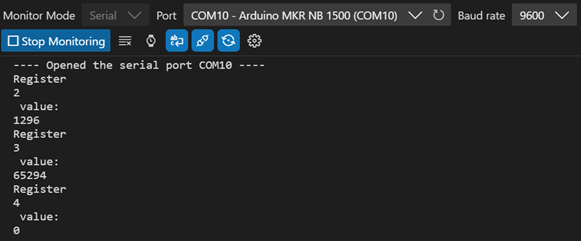
\includegraphics[scale=0.7]{images/Read_register.png}
\caption{Reading Register Values}
\label{fig:x Reading Register}
\end{figure}
\subsection{Reading Analog Data} 
 
\begin{figure}[htbp]
\centering
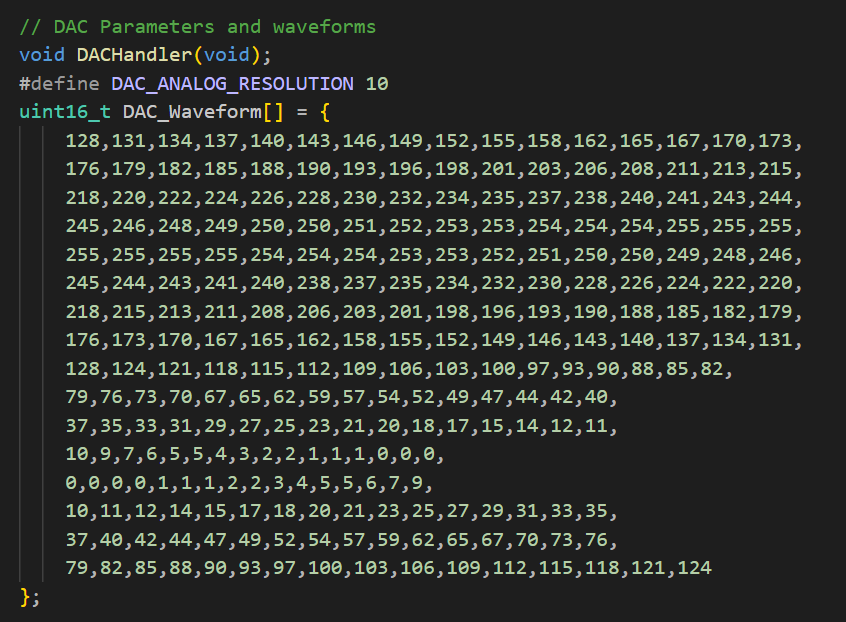
\includegraphics[scale=0.5]{images/DACWaveform.png}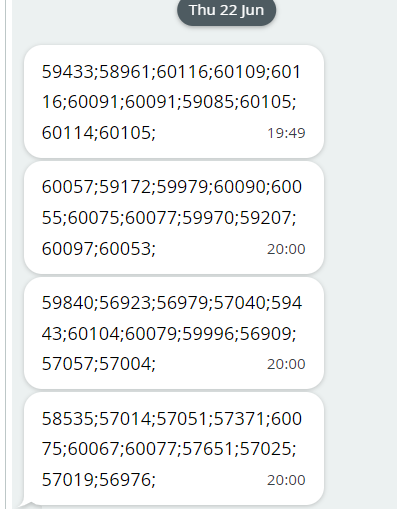
\includegraphics[scale=0.6]{images/SamplesCLOUD.png}
\caption{DAC Waveforms and Output}
\label{fig:x DAC_Waveforms}
\end{figure}
The process of generating an analog waveform using a Digital-to-Analog Converter (DAC) entails generating a sequence of digital values that align with the intended waveform.These digital values are then transmitted to the DAC to generate the corresponding analog signal. In our case, we generated a DAC waveform with a resolution of 10 bits and obtained the resulting output from the ADC, as depicted in the accompanying figure \ref{fig:x DAC_Waveforms}.
\section{Arduino IoT Cloud}
Arduino IoT Cloud serves as a platform facilitating seamless and secure connectivity between Arduino-based projects and the internet. It empowers the creation of IoT applications by simplifying the establishment of remote monitoring, control, and data collection for devices and sensors. The API Key tab grants access to essential credentials such as the client ID and secret keys, which are automatically generated upon thing creation. The ThingID is retrievable from the metadata section. Once the hardware integration with the cloud is finalized, it becomes possible to incorporate variables into things. These global variables are assigned specific IDs, enabling data reading and writing on the things using the Device ID, Thing ID, and Variable ID.
At initial attempt, we have to declare a total of four variables in our Arduino Cloud platform. These cloud variables name, type, operation, and ID has been listed in Table \ref{tab:Cloud variable} for a push button based data acquisition. Later, we have designed the variables and things to measure the RMS(I1,I2,I3), and RMS (V1,V2,V3), including Sync Period, and testing with NB-IoT. These variables dashboard has been shown in figure \ref{fig:x Cloud Variables}. 

\begin{table}[htbp]
  \centering
  \caption{Arduino Cloud variables for a single push button }
  \label{tab:Cloud variable}
   \adjustbox{width=1\textwidth, height=0.05\textheight}{
  \begin{tabular}{|c|c|c|c|}
    \hline
    \textbf{Cloud Variables} & \textbf{Variable Type} & \textbf{Variable Permission} & \textbf{Variable ID} \\
    \hline
    cloudADCParam  & Character string & Read \& Write & 58dd6174-6fe3-4173-9b38-154e90699878\\
    \hline
    cloudData  & Float  &  Read \& Write & 22a67deb-cf99-4950-8720-e62bff7a90cb \\
    \hline
    cloudPB  & Boolean & Read \& Write & 68d94ebb-f01e-4a8a-a799-41d945d9dbcf \\
    \hline
    cloudSamples  & Character string  & Read \& Write & f06b9506-f7c8-473a-af4c-8b4dd028d455  \\
    \hline
  \end{tabular}
  }
\end{table}

\begin{figure}[htbp]
\centering
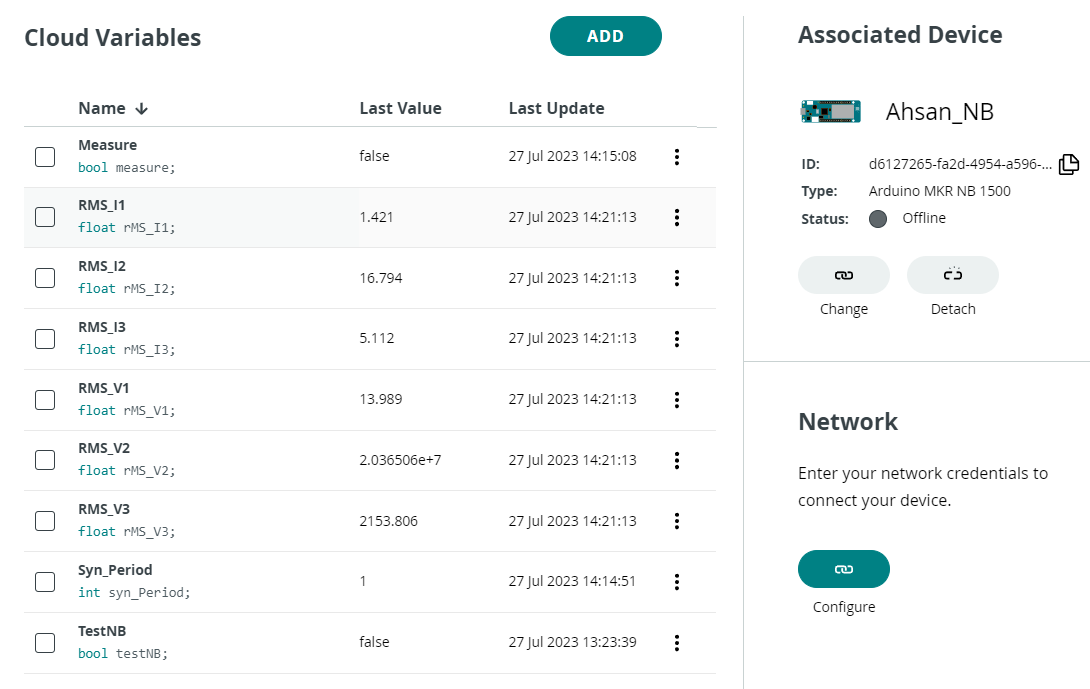
\includegraphics[scale=0.55]{images/Cloud Variables.PNG}
\caption{Cloud Variables for measuring RMS}
\label{fig:x Cloud Variables}
\end{figure}
In order to handle Arduino IoT Cloud Devices, Things, Properties, and Timeseries, the \href{https://www.arduino.cc/reference/en/iot/api/}{Arduino IoT Cloud API} offers a set of APIs. Any HTTP Client can be used to call this API. Also, Arduino Cloud provides a Web Editor which have a collection of code examples and libraries that we can use as a starting point for our IoT projects. This web editor helped us initially and running quickly without having to write code from scratch. The cloud dashboard offers a range of distinctive features that set it apart from other platforms. These include Data Visualization, widgets for easy configuration, a user-friendly Drag-and-Drop Interface, Real-Time Updates, the ability to set up Alerts and Notifications for multiple devices, and the flexibility for Customizations. These unique attributes played a significant role in our decision to select this platform for our project.

\section{Matlab WebAccess} 
\subsection{Data Reading and Writing}
To retrieve data from a web cloud using a MATLAB script, we can utilize various methods such as making HTTP requests, accessing APIs, or scraping web content. In the script of figure \ref{fig:x Matlab Response2}, the \textbf{‘webread’} function is used to make a \textbf{GET} request to the specified URL. The response from the API is a JSON object, which is then displayed in the MATLAB command window.\textbf{‘weboptions’} is a function in MATLAB that allows us to configure options for making HTTP requests using functions like webread or webwrite to interact with web services and APIs. It provides a way to customize various aspects of the request, such as headers, query parameters, timeouts, and more. This function is useful when we need to tailor the behavior of our HTTP requests to match the requirements of the web service we are interacting with.
The \textbf{‘strcat’} function in MATLAB is used to concatenate strings together. It takes multiple input arguments, which are strings or character arrays, and combines them into a single string.\par
\begin{figure}[htbp]
\centering
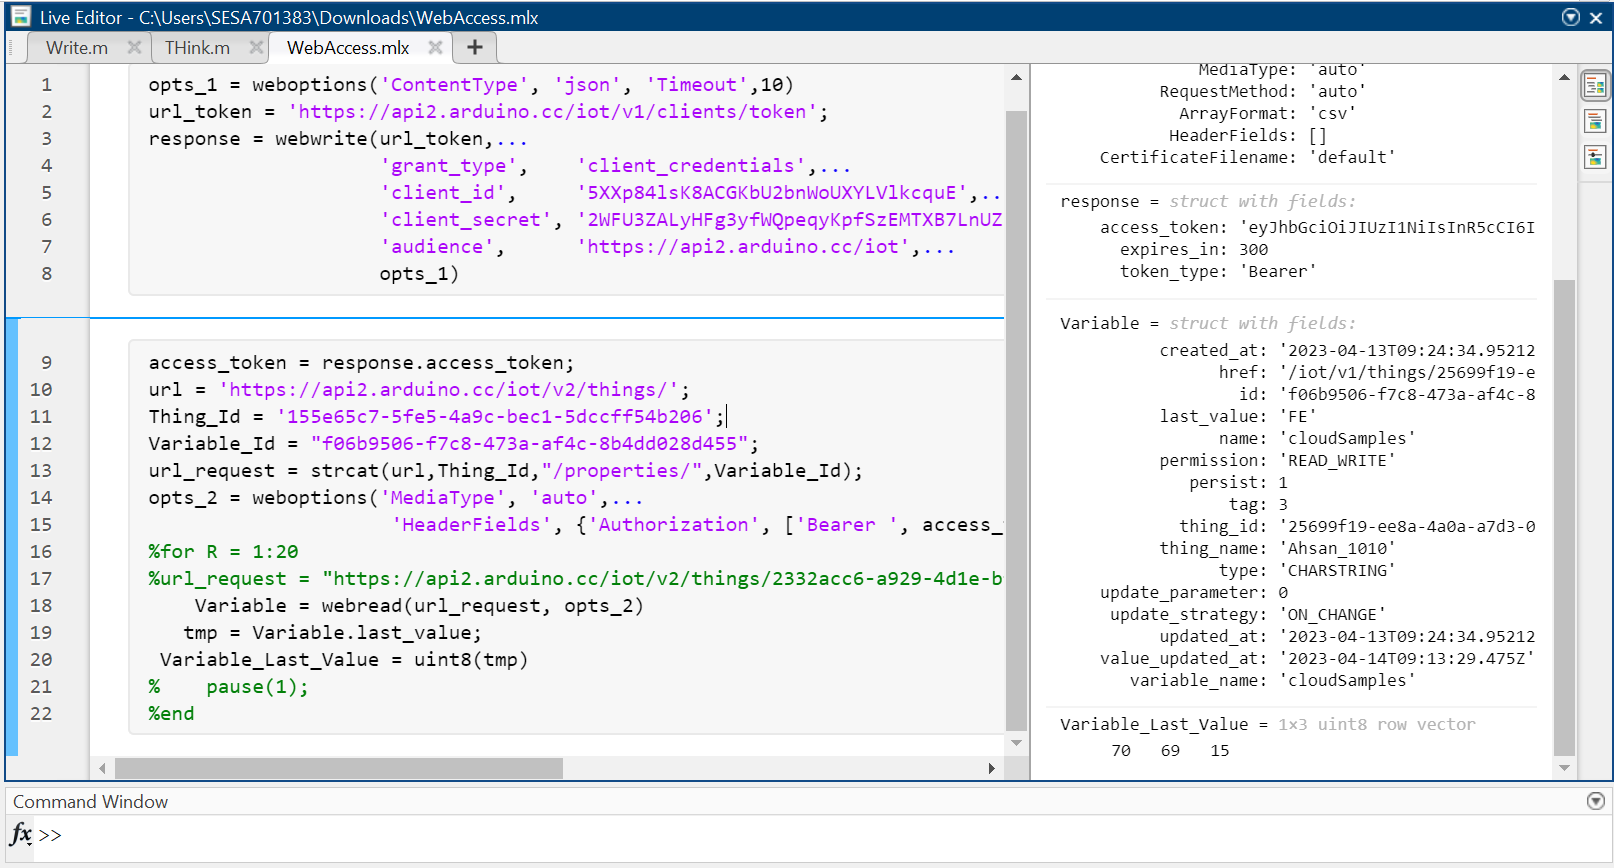
\includegraphics[scale=0.5]{images/Matlab Response2.PNG}
\caption{Data Reading from Cloud with Matlab}
\label{fig:x Matlab Response2}
\end{figure}
The \textbf{‘webwrite’} function in MATLAB is used to make HTTP \textbf{POST} requests and send data to a web service or API. It allows us to send data in various formats, such as JSON or form data, to a specified URL. Our data authentication process through MATLAB has few steps. At first, we need to get a authentication token which has been shown in the previous figure. Data reading from Arduino Cloud has been also depicted in previous figure. Then we write data to Arduino cloud variables by using webwrite, PUT command has been used in the weboption function. Finally, we have succeed to read historic data from the cloud and PUT the calculated unbalanced RMS values to the cloud variables demonstrated in figure \ref{fig:x Historical}.
\begin{figure}[htbp]
\centering
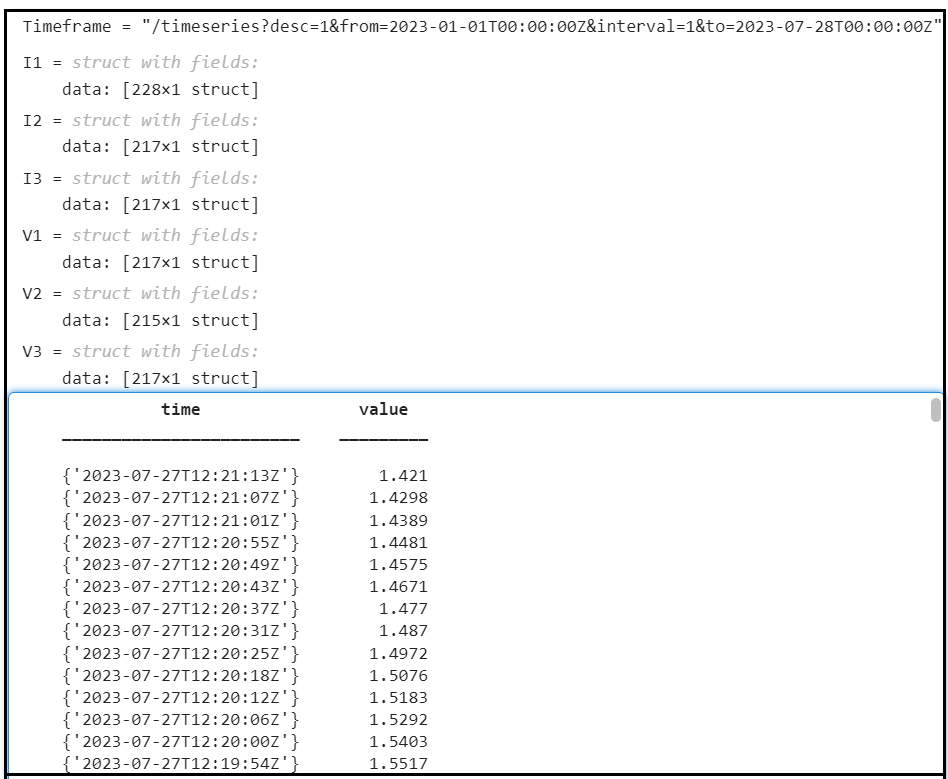
\includegraphics[scale=0.450]{images/HistoricData.PNG} 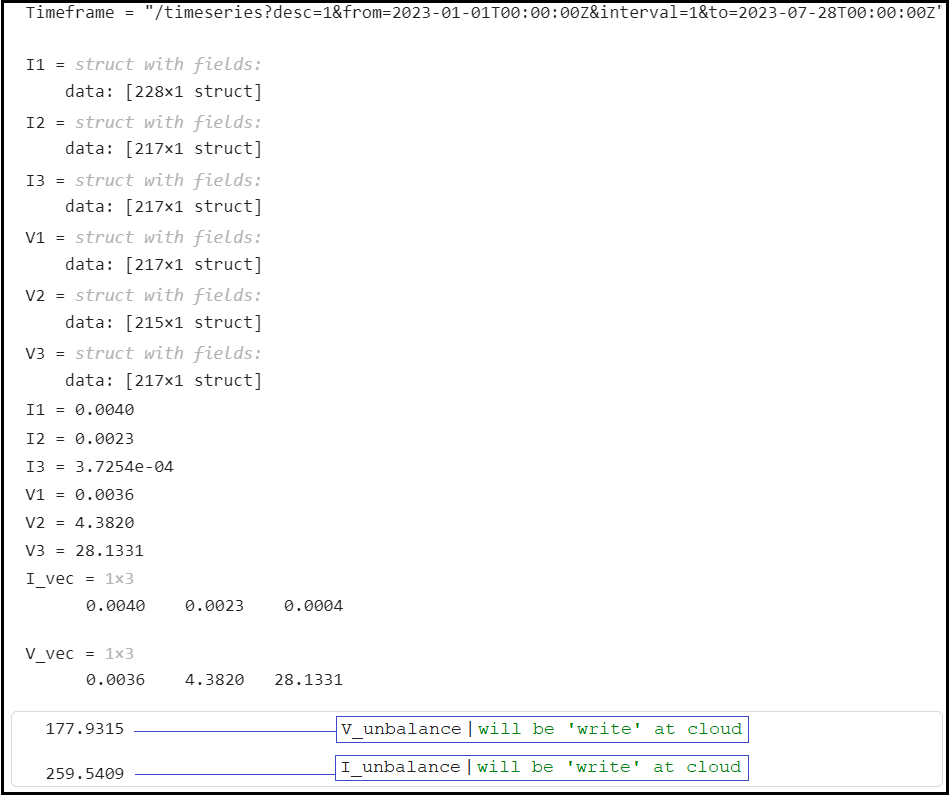
\includegraphics[scale=0.435]{images/UnbalancedWrite.PNG}
\caption{Historical data reading and writing unbalanced data}
\label{fig:x Historical}
\end{figure}
\subsection{Postman API}
During the MATLAB session we tested our API in \href{https://www.postman.com/}{Postman}. It allows us to create and send various types of HTTP requests, including GET, POST, PUT, DELETE, and more. We can specify request headers, parameters, body content, and authentication details. It supports various authentication methods, including basic authentication, API keys, OAuth 2.0, and more. We have used OAuth 2.0 authentication methos. Reading data from Arduino cloud by using GET API method has been demonstrated in figure \ref{fig:x Postman}.
\begin{figure}[htbp]
\centering
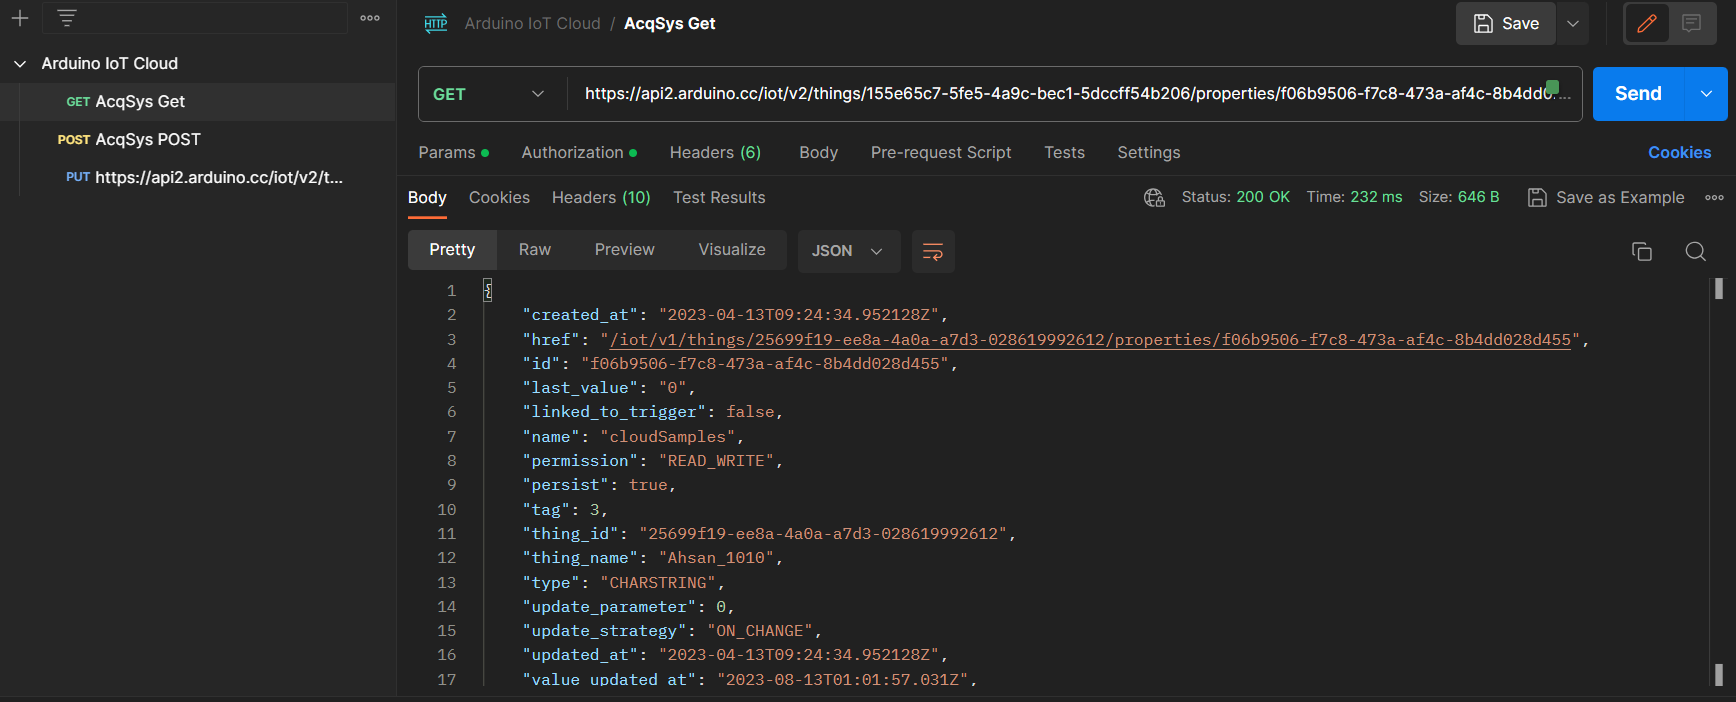
\includegraphics[scale=0.460]{images/postman.png} 
\caption{Configuring HTTP request through Postman API}
\label{fig:x Postman}
\end{figure}
\section{RTOS} 
\href{https://freertos.org/}{FreeRTOS} (Real-Time Operating System) is an open-source real-time operating system kernel for embedded systems. It provides a compact and efficient platform for developing applications that require precise timing and synchronization, making it well-suited for a wide range of embedded and IoT devices. FreeRTOS provides a manual for the mastering in Real Time Kernel included in \cite{FreeRTOS}. Also we studied another article to understand about FreeRTOS \cite{UnderstandingRTOS}. 

\subsection{Source files of FreeRTOS}
The fundamental FreeRTOS source code is present within only two C files that are universal across all FreeRTOS ports.  Tasks.c and List.c are both of them, and they can be found in the FreeRTOS/Source directory, as illustrated in Figure \ref{fig:x RTOS Tree}. 

\begin{figure}[htbp]
\centering
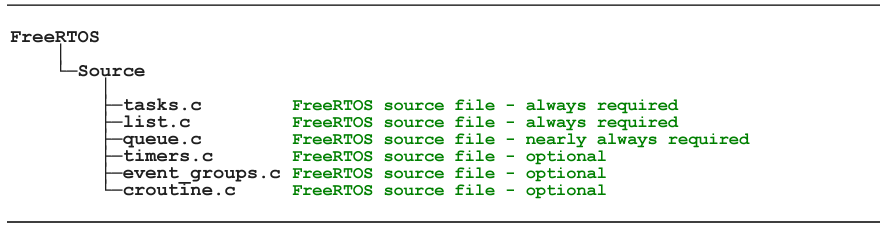
\includegraphics[scale=0.9]{images/FreeRTOS.png}
\caption{Core FreeRTOS source files in directory tree }
\label{fig:x RTOS Tree}
\end{figure}
The other source files also reside in the same directory as these two. The 3rd file from the source \textbf{‘queue.c’} provide a way for tasks to send and receive messages or data packets to/from each other in a thread-safe manner. It contains the implementation of the queue-related functions and data structures, including creating and deleting queues, sending and receiving data, blocking and unblocking tasks, and managing queue resources. Fourth one \textbf{‘timers.c’} provides the functionality for creating and managing software timers. Software timers are a key feature in FreeRTOS that allow tasks to be scheduled to run at specific intervals or after a certain delay, without the need for hardware timers. Fifth RTOS file from figure \textbf{‘event\_groups.c’} used for inter-task communication and synchronization in a multitasking environment. Event groups allow tasks to wait for specific combinations of events to occur. Tasks can set or clear individual bits within an event group, and other tasks can wait for a specific combination of bits to be set before continuing their execution. For the last one
\textbf{‘croutine.c’}, co-routines are a way to achieve cooperative multitasking within a single task context, allowing tasks to yield execution voluntarily to other tasks without relying on a preemptive scheduler. Co-routines are suitable for systems with limited resources, where full preemptive multitasking might be too heavyweight. They provide a mechanism for tasks to work together in a cooperative manner, sharing the CPU time based on their own scheduling decisions.\par
\vspace{0.5cm}\par
On the other hand, Heap management is an essential component for dynamic memory allocation required by tasks, queues, semaphores, and other kernel objects. Each task in FreeRTOS requires its own stack and potentially some heap space, depending on its memory requirements. In our firmware we used \textbf{‘heap\_4bis.c’}, which Implements thread-safe memory allocation using a critical section or mutex. It uses a block of memory provided by the application for the heap. The two main functions are \textbf{‘pvPortMalloc()’} and \textbf{‘pvPortFree()’}. These functions are used to dynamically allocate and deallocate memory from the heap.

\subsection{Header files of FreeRTOS}

A source file utilizing the FreeRTOS API should begin by including \textbf{‘FreeRTOS.h’}, followed by the appropriate header file housing the prototype for the utilized API function. These header files could be ‘task.h’,‘queue.h’,‘semphr.h’,‘timers.h’, or ‘event\_groups.h’. FreeRTOS.h is the main header file that we include in our OS. It provides access to the FreeRTOS API functions, data types, and macros. It also includes other necessary header files.
\textbf{‘task.h’} defines the functions and data structures for task management, creation, deletion, priority, and synchronization. queue.h provides the API for creating, using, and managing message queues. \textbf{‘semphr.h’} defines the API for creating and using semaphores for task synchronization and resource sharing. \textbf{‘event\_groups.h’} contains the API for creating and using event groups for inter-task communication and synchronization. \textbf{‘portmacro.h’} contains macros and functions that are specific to the architecture or port being used. This is where port-specific definitions and inline assembly might be defined. \textbf{‘FreeRTOSconfig.h’} contains architecture-specific or platform-specific configuration header files. These files allow us to configure various aspects of FreeRTOS behavior, such as tick rate, memory allocation scheme, and more. \textbf{‘croutine.h’} provides definitions and macros for co-routines, which are a lightweight form of multitasking. \textbf{‘portable.h’} has been included within a port layer's implementation to provide further port-specific definitions or macros.

\begin{figure}[htbp]
\centering
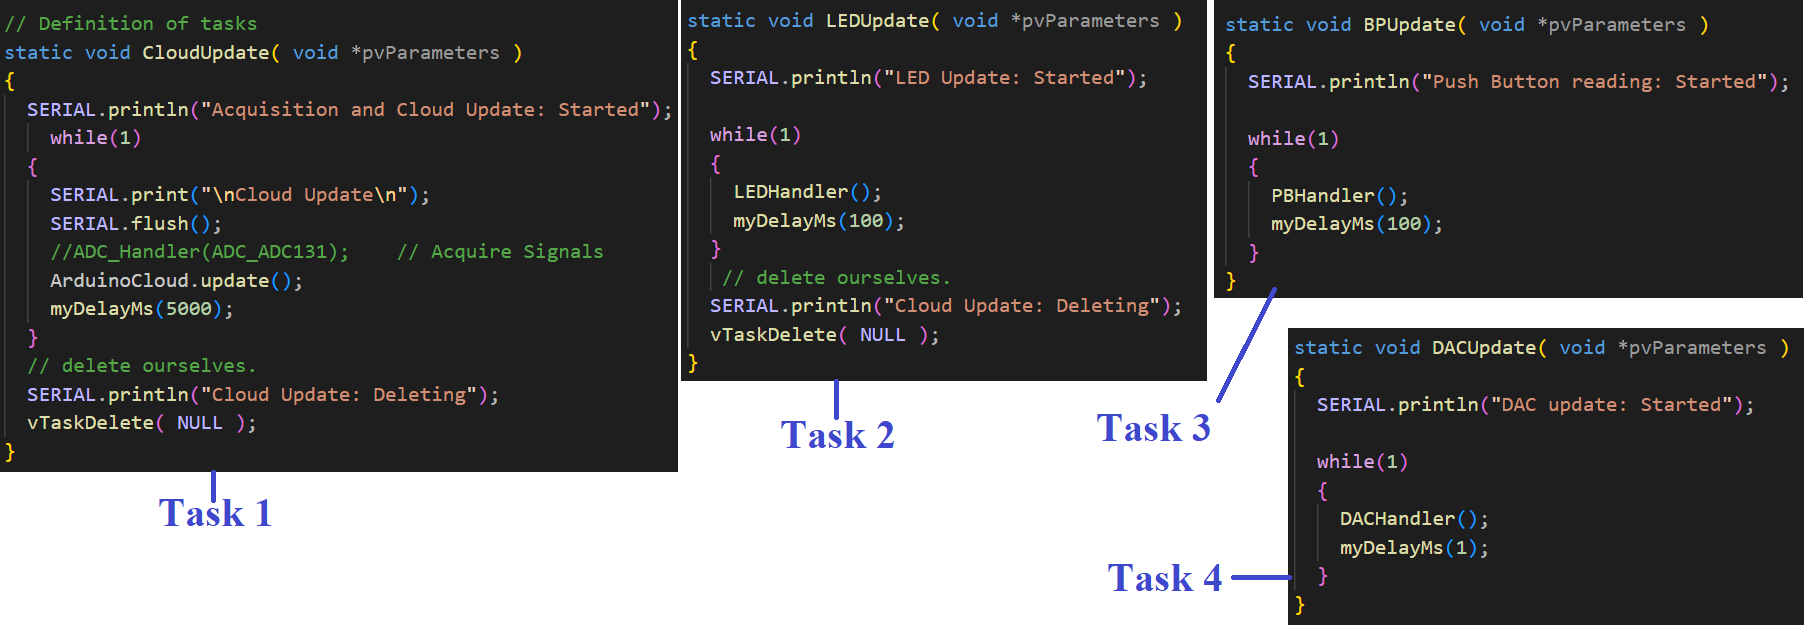
\includegraphics[scale=0.45]{images/Task1.png}
\caption{Task definition for acquisition system}
\label{fig:x RTOS Def}
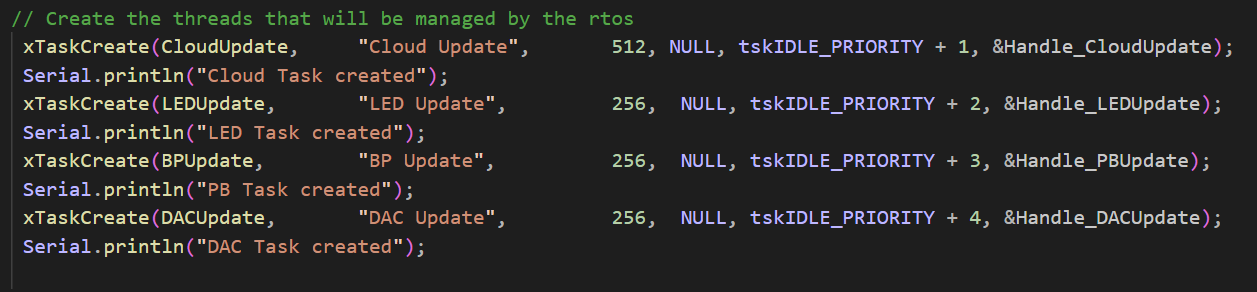
\includegraphics[scale=0.65]{images/RTOS_task.png} 
\caption{Scheduling the Tasks}
\label{fig:x RTOS Task}
\end{figure}
Task definition of our firmware has been depicted in the figure \ref{fig:x RTOS Def}, where we have created four different tasks CloudUpdate, LEDUpdate, BPUpdate, and DACUpdate. In figure \ref{fig:x RTOS Task}, all these four task scheduling has been depicted. Within this particular section, the task labeled Cloud Update commands a memory allocation of 512 bytes due to its elevated priority. Conversely, the remaining tasks have been assigned 256 bytes each, following a priority hierarchy where the sequence is as follows: LED Update $>$ BP Update $>$ DAC Update.


\section{Simulink Embedded Algorithm} 
Algorithms that are implemented on embedded systems, which are specialized hardware platforms made to carry out certain activities or operations, are referred to as embedded algorithms. Field-programmable gate arrays (FPGAs), microcontrollers, digital signal processors (DSPs), and application-specific integrated circuits (ASICs) are a few examples of hardware with limited computational resources that these algorithms are often made to operate efficiently on. To implement an algorithm in Simulink, a graphical representation of the algorithm's stages and calculations must be made. Simulink offers a visual platform for creating and modeling dynamic systems that incorporate methods from several fields, including signal processing, control systems, image processing, and more. 

\par
\begin{figure}[htbp]
\centering
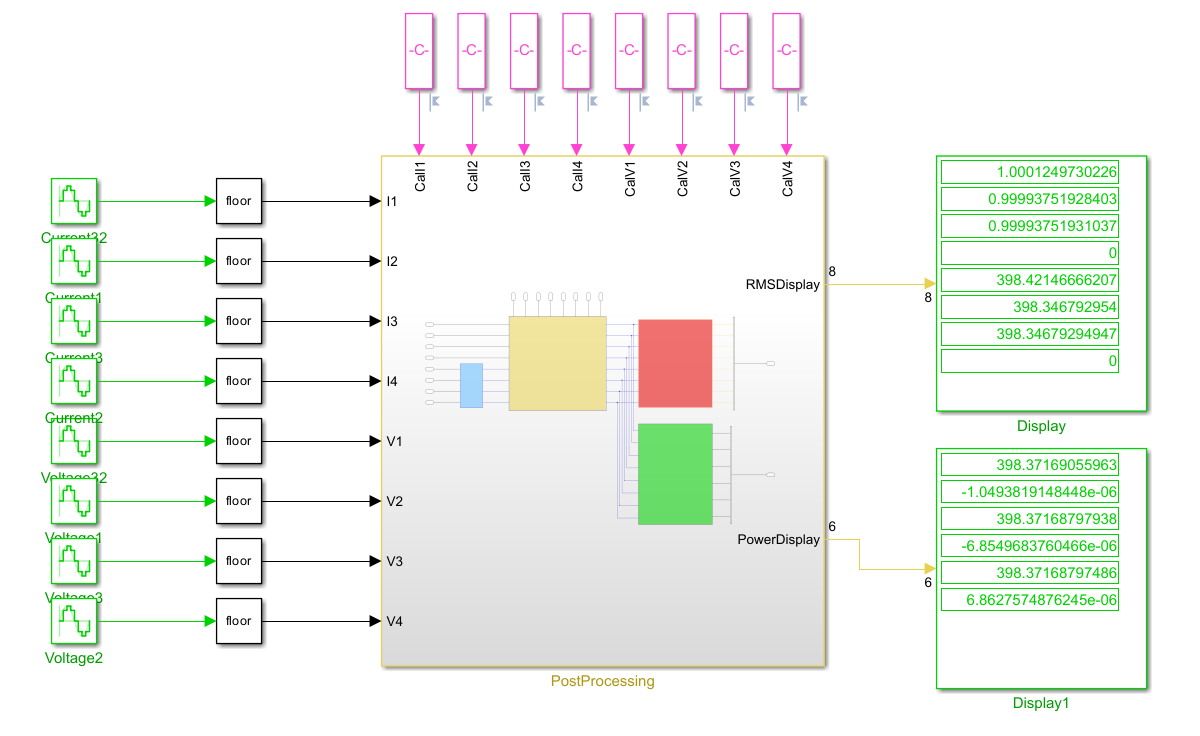
\includegraphics[scale=0.33]{images/Feature Extraction.png}
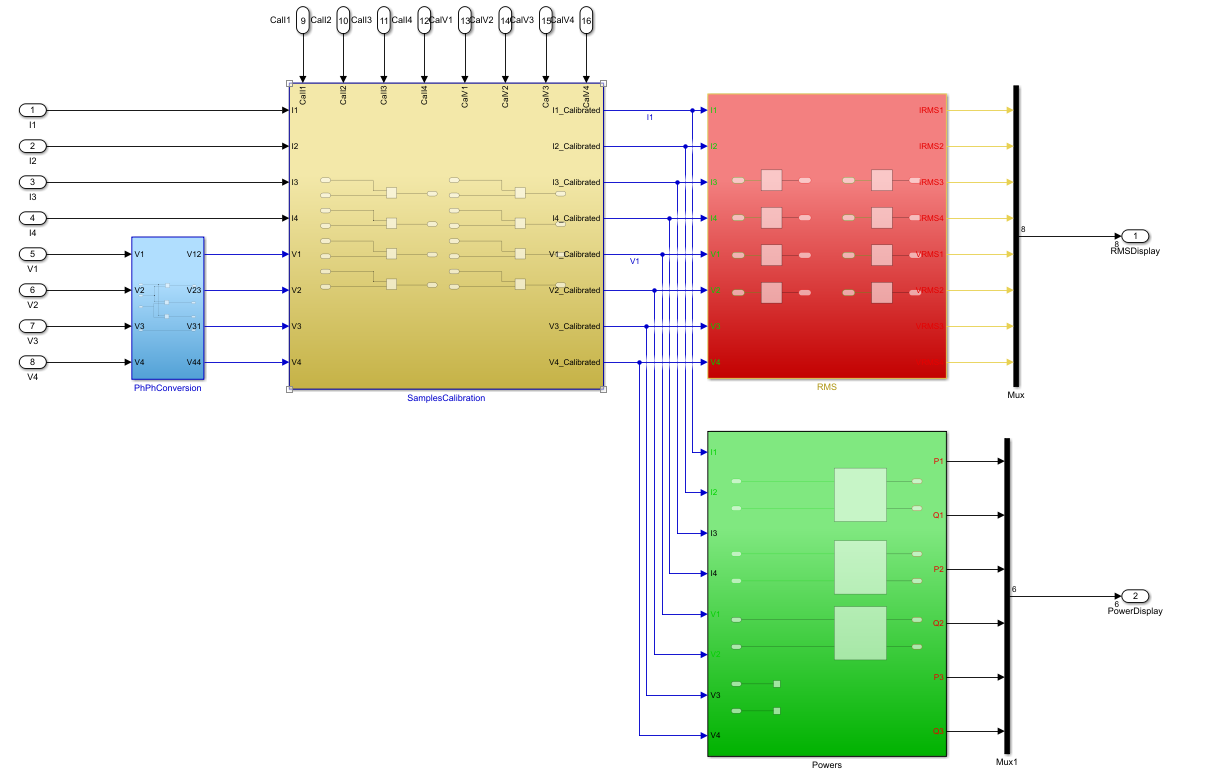
\includegraphics[scale=0.33]{images/PostProcessing.png}
\caption{Embedded Algorithm for Acquisition System}
\label{fig:x Embedded Algorithm}
\end{figure}

In the figure \ref{fig:x Embedded Algorithm}, we have designed an embedded algorithm in simulink to serve the RMS calculation purpose for our acquisition system.In the left block, there are 8 distinct analog signals originating from 8 channels of the ADS131M08. Additionally, 8 unique calibration factors are directed towards the \textbf{PostProcessing } block. The \textbf{RMSDisplay} and \textbf{PowerDisplay} blocks depict the computed outcomes during simulation. On the right block, the PostProcessing segment has been constructed, within which a \textbf{PhPhConversion} block (depicted as Blue) is utilized to analyze the three-phase voltages. The variance across two lines as the phases intersect at an angle is commonly termed as the line-to-line voltage. In the PhPhConversion block, the calculation of the differences between V1, V2, and V3 is carried out, with V4 representing the ground reference.
In the \textbf{SamplesCalibration} block (depicted as Yellow), all these analog signals undergo calibration using the 8 distinct calibration factors. Subsequently, the RMS is determined by the Red Block, while the Power values are computed by the Green Block.\par
\vspace{0.5cm}

In Figure \ref{fig:x Cal_RMS Block }, the left illustration represents our \textbf{SamplesCalibration} process, wherein every individual sample is divided by its corresponding calibration factor. Meanwhile, the right depiction showcases the application of the \textbf{Moving RMS} block. This block computes the moving RMS of the input signal for each channel independently over a specific time duration. The block squares the data samples, multiplies them by a series of weighting factors, and then adds the weighed data in the exponential weighting process. The RMS is then calculated by the block by calculating the sum's square root.\par

\begin{figure}[htbp]
\centering
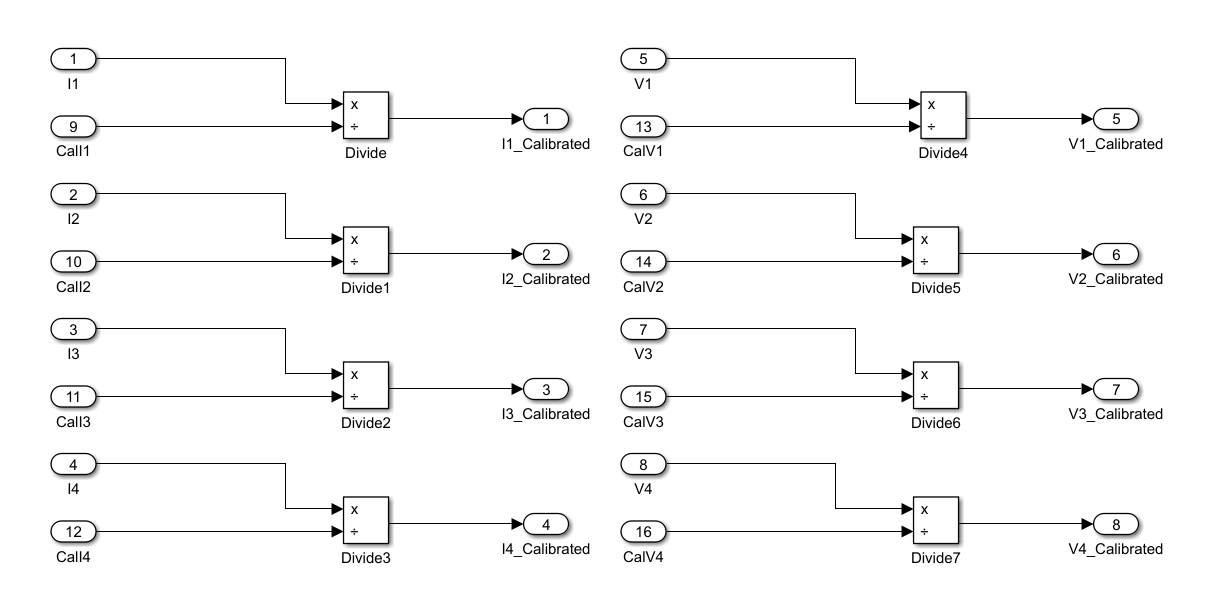
\includegraphics[scale=0.4]{images/Sample_Calibration.PNG}
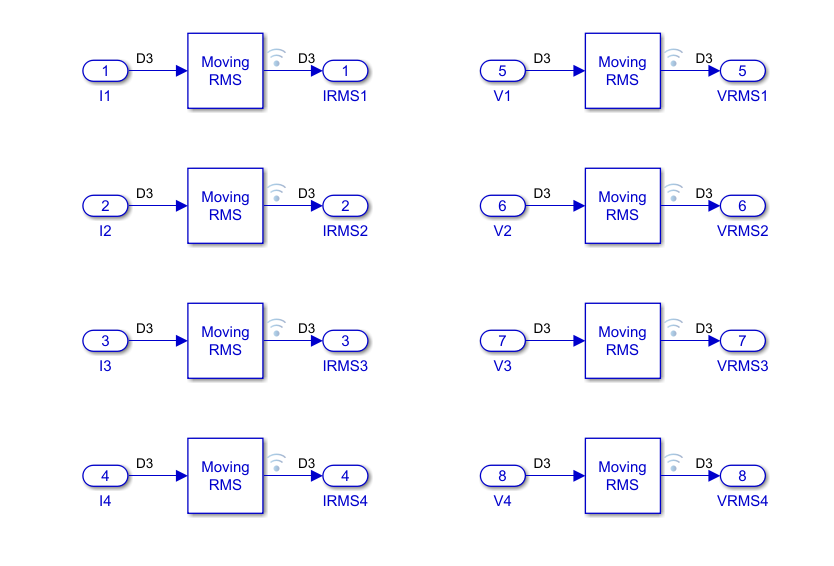
\includegraphics[scale=0.4]{images/RMS.png}
\caption{Calibration and RMS Calculation Block}
\label{fig:x Cal_RMS Block }
\end{figure}

\textbf{Simulink Embedded Coder:}
We can create effective, condensed, and optimized C and C++ code from our Simulink models and Stateflow diagrams using this robust tool from MathWorks. In particular for embedded systems and real-time applications, it is a crucial part of the MathWorks ecosystem. We can automatically create code for a range of hardware targets, including microcontrollers, CPUs, and FPGAs, thanks to Simulink Embedded Coder.


 \begin{figure}[htbp]
\centering
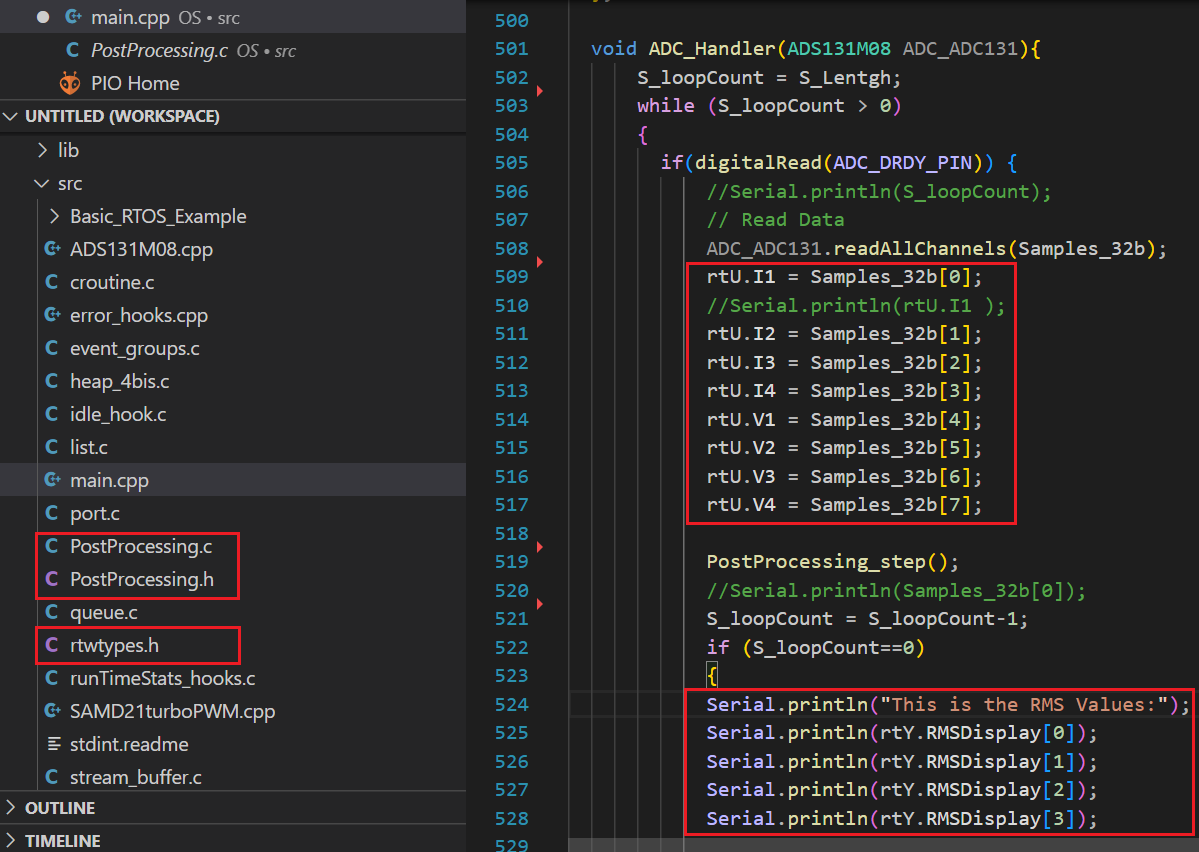
\includegraphics[scale=0.6]{images/RMS Calculation.PNG}
\caption{Utilyzing Simulink generated code in our firmware}
\label{fig:x Algorithm RMS}
\end{figure}

We have generated C code of PostProcessing block from our designed algorithm.Three generated files \textbf{‘PostProcessing.c’},\textbf{‘PostProcessing.h’}, and \textbf{‘rtwtypes.h’} has been added to the firmware shown in figure \ref{fig:x Algorithm RMS}. The purpose of rtwtypes.h is to define platform-independent data types that ensure consistent data representation across different target platforms. These data types are used in the generated code to ensure that the behavior of the Simulink model is preserved when running on different hardware. \textbf{rtU.I} represents the 32 bit analog current samples, and \textbf{rtU.V} represents the voltage samples. The function \textbf{PostProcessing\_step()} runs our designed algorithm for these sample data calculation. Then \textbf{rtY.RMSDisplay} is the output which will be displayed in our serial monitor. We have tested the RMS for the 1st channel by supplying 1amp current to the ADC, and this Simulink Algorithm represented 0.991 amp in serial monitor after calculation.

\nomenclature{$IDE$}{Integrated Development Environment}
\nomenclature{$RTOS$}{Real Time Operating System}
\nomenclature{$CRC$}{Cyclic Redundancy Check}
\nomenclature{$OSR$}{Oversampling Ratio }
\nomenclature{$HTTP$}{Hypertext Transfer Protocol}
\nomenclature{$DSP$}{Digital Signal Processors}
\nomenclature{$ASIC$}{Application-specific Integrated Circuits}
\nomenclature{$FPGA$}{Field-programmable Gate Arrays}





\chapter{Result Analysis}\label{Result}

%\section{Result Analysis} 
\section{Laboratory Setup}
We conducted thorough testing of our developed board at Schneiders Electrical Lab. The laboratory setup is visually explained in Figure \ref{fig:x Lab}. The components labeled by red squares were employed for these tests. The TA325 flex current probe facilitated current sensing and transmission to the ADS131M08. Additionally, the Rogowski coils, coloured in red, green, and blue, were employed to sense current along the three-phase lines. Furthermore, the OMICRON CMS 356 voltage and current amplifier served as our testing equipment. It was connected to the Schneiders Real Time current and voltage simulator application. To verify current, a multimeter was utilized, and four oscilloscope probe has been connected with the acquisition board to visualise the clock, data ready, data out and sample signals.
\begin{figure}[htbp]
\centering
\includegraphics[scale=0.06]{images/LabSetup.jpg}
\caption{RMS Current measuring in Lab}
\label{fig:x Lab}
\end{figure}
\section{Calibration and Validation}
We have defined 8 calibration factors in our firmware. To put those factors we have analysed the AC current samples through our serial monitor. We have supplied 1 Amp current and found analog samples shown in figure \ref{fig:x AC Current}. 

\begin{figure}[htbp]
\centering
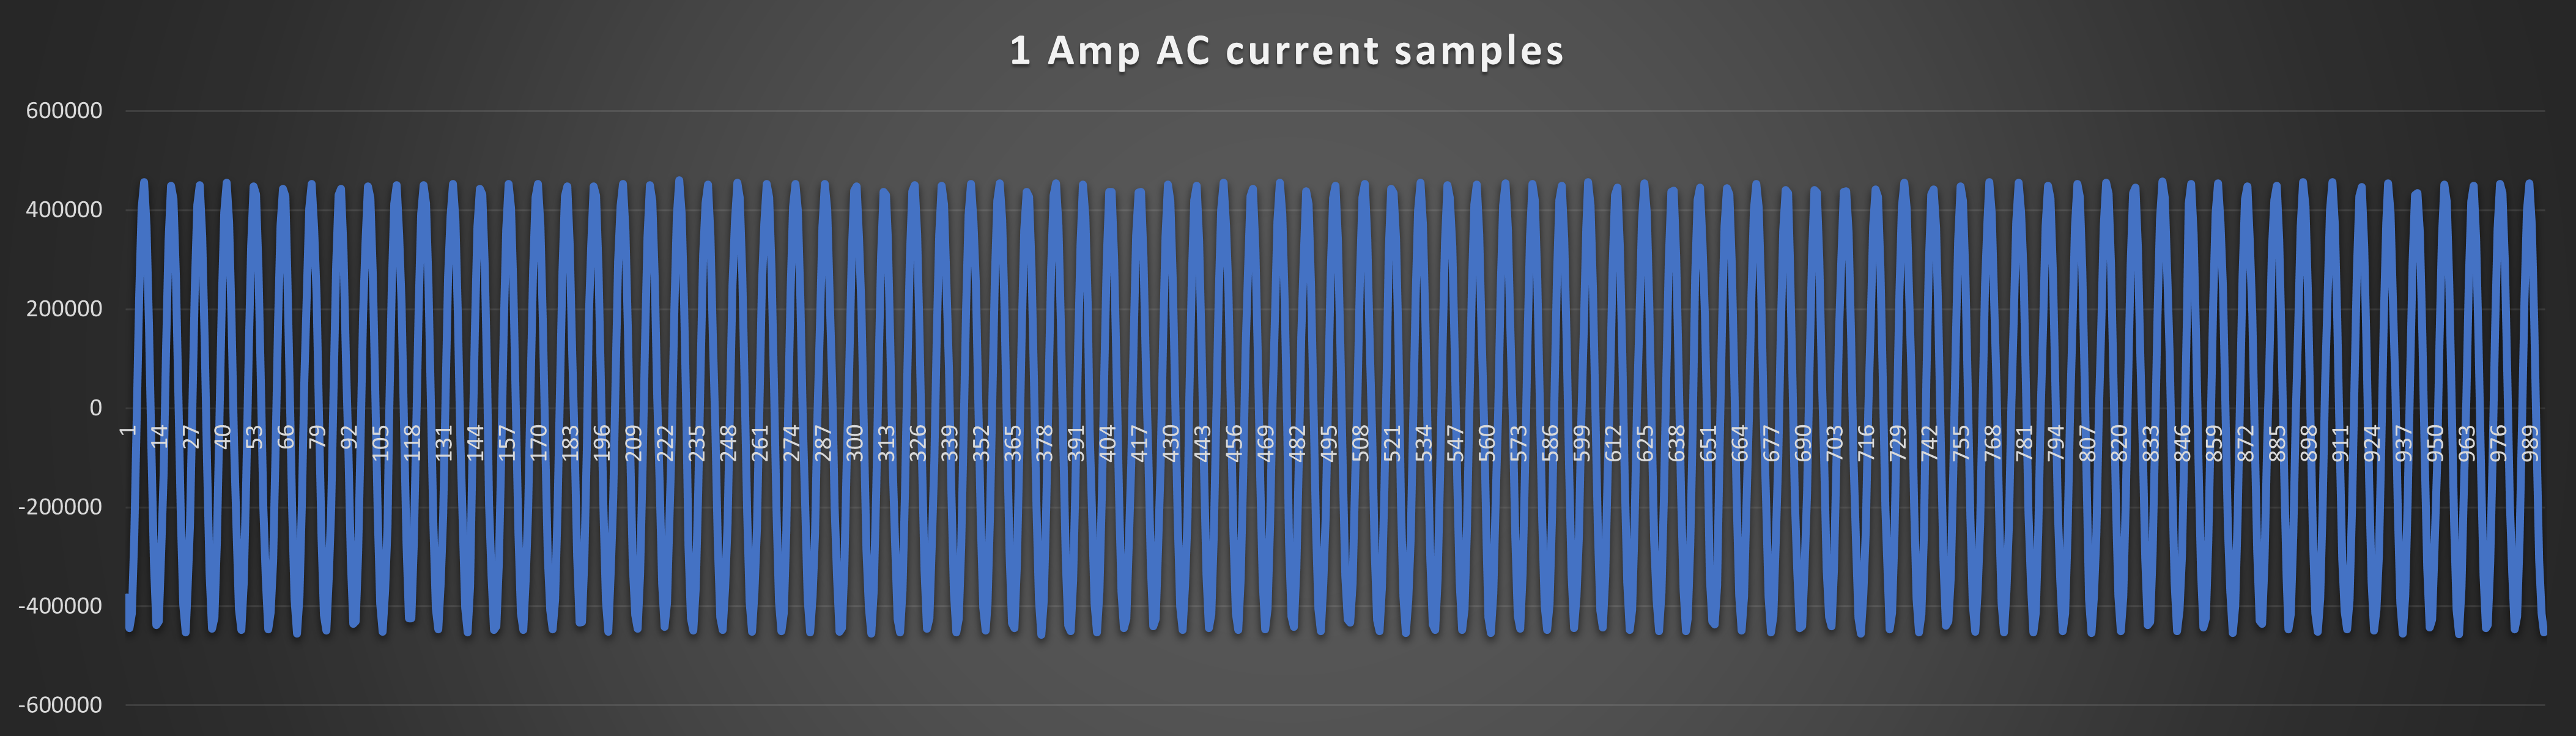
\includegraphics[scale=0.4]{images/AC_Current.png}
\caption{AC current samples}
\label{fig:x AC Current}
\end{figure}
We know that, 
\begin{align}\label{Eqn RMS}
I_{rms} = I_{peak} / \sqrt{2}
\end{align}
After analysing the AC current samples from one channel, maximum sample value was 460687. So, $I_{peak}=460687$, and applying to the equation \ref{Eqn RMS} we find the RMS value $I_{rms}=325754.9017$, what we set the calibration factor \textbf{rtU.CalI1}. Additionally, from the AC currents samples figure we can assume the data rate was approximately 4KSPS. For the voltage calibration lets have a look in figure \ref{fig:x Schematic} voltage measurement input section, each line of voltage have six 500k resistors at $V_{in}$ side, and one 4.7k resistor at $V_{out}$ side. So it makes:
\begin{align}\label{Eqn Resistance}
\frac{V_{out}}{V_{in}}=\frac{4.7k}{4.7k+3000k}=\frac{4.7k}{3004.7k}
\end{align}

Now, our reference voltage $V_{Ref}= 1.25V$, and the ADC resolution is 24 bit, as a consequence $2^{23}$ is the highest bit of ADC. We can put equation \ref{Eqn Resistance} data for making calibration voltage which will take placed by \textbf{rtU.CalV1}: 
\begin{align}\label{Eqn Cal}
V_{Cal}=\frac{V_{Ref}\times3004.7}{2^{23}\times 4.7k}
\end{align}


\section{Analysing Signal in Oscilloscope} 
\begin{figure}[htbp]
\centering
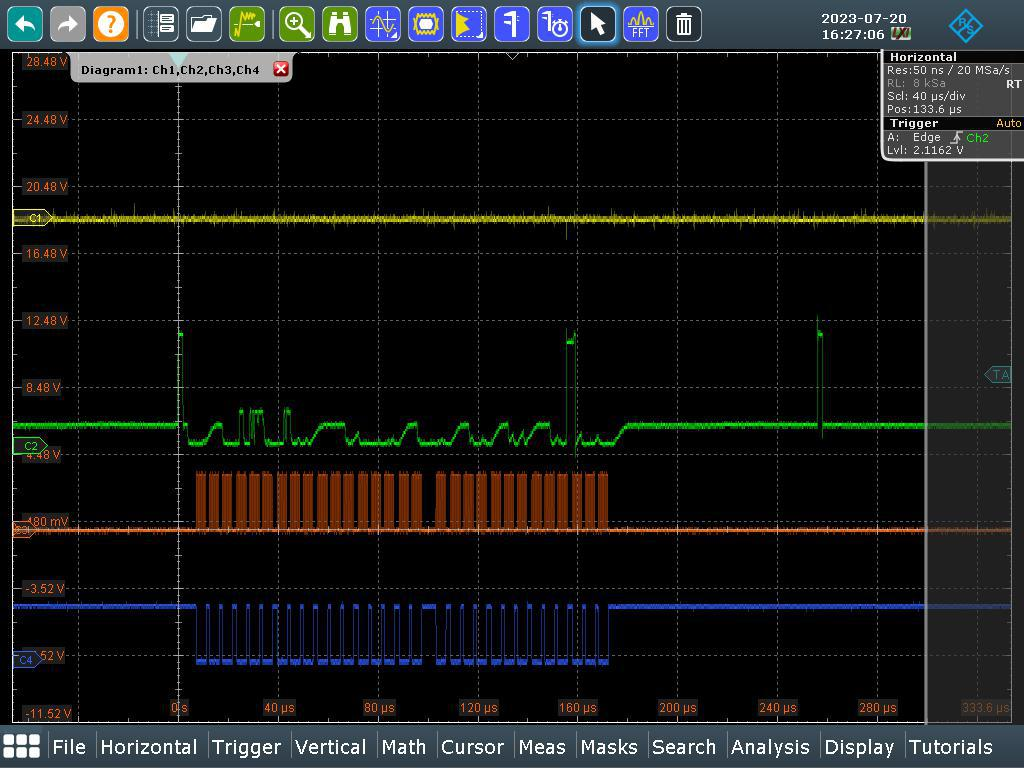
\includegraphics[scale=0.195]{images/Output 1.png}
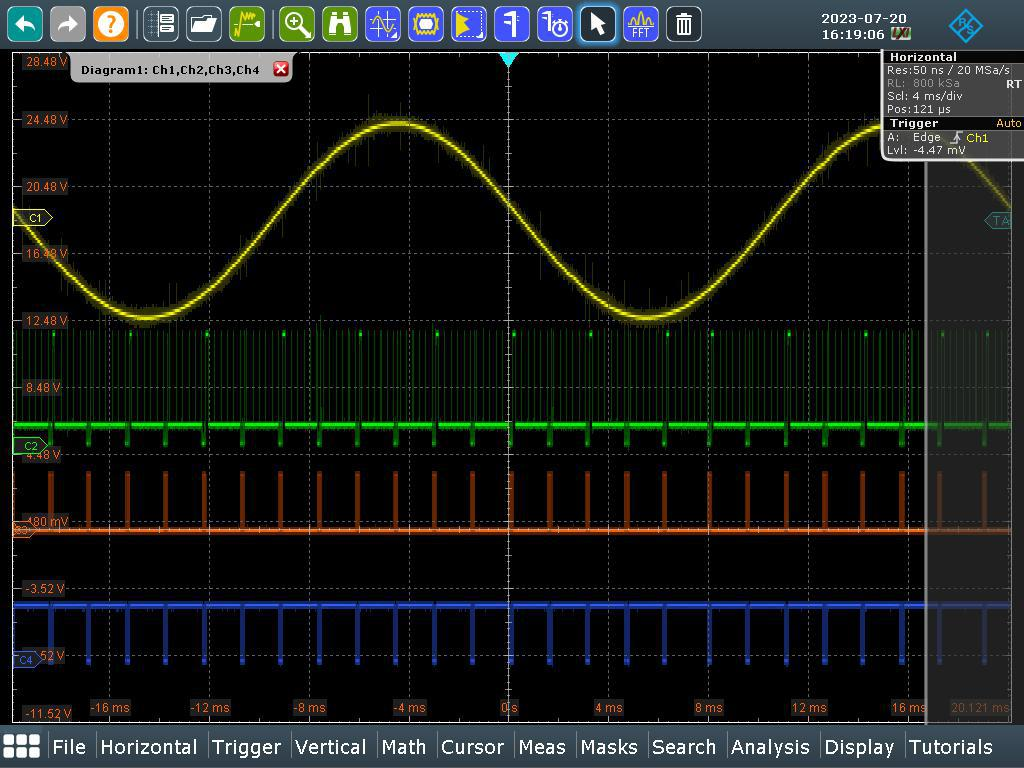
\includegraphics[scale=0.26]{images/Output 2.png}
\caption{Signals in Oscilloscope}
\label{fig:x Output1}
\end{figure}
Output from oscilloscope has been depicted in figure \ref{fig:x Output1}, where \textbf{Yellow} Signal represents Current sample (single channel), \textbf{Green} Signal represents the Data Ready, \textbf{Brown} Signal represents the master Clock, and \textbf{Blue} Signal represents the Data Output.


\section{IoT Cloud Dashboard} 
Our finalized IoT cloud dashboard is visually presented in Figure \ref{fig:x IoT_Dashboard}. The left figure showcases the RMS value within a balanced operational state, while the right figure highlights the RMS value under unbalanced conditions. Upon initiating data acquisition by pressing the dedicated button, the acquired data is synchronized at regular intervals, precisely set by us at a 1-second interval. 
\begin{figure}[htbp]
\centering
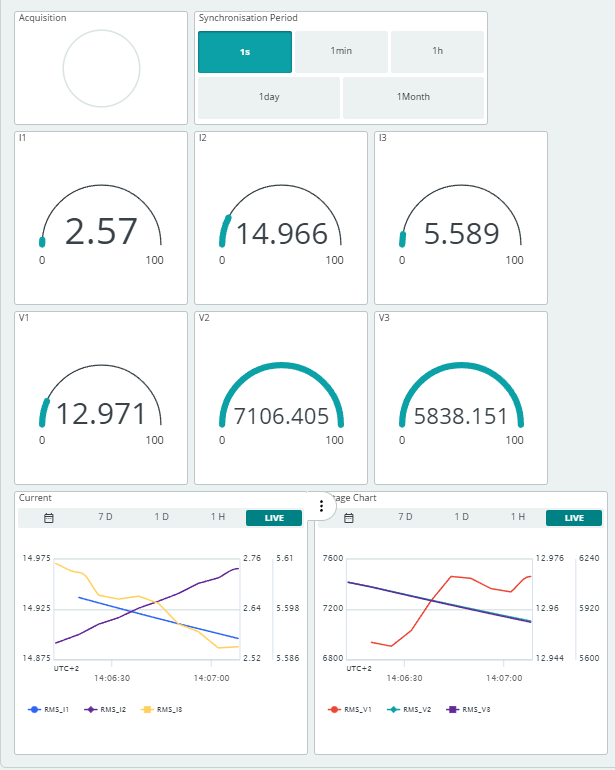
\includegraphics[scale=0.59]{images/IoT_Dashboard.png}
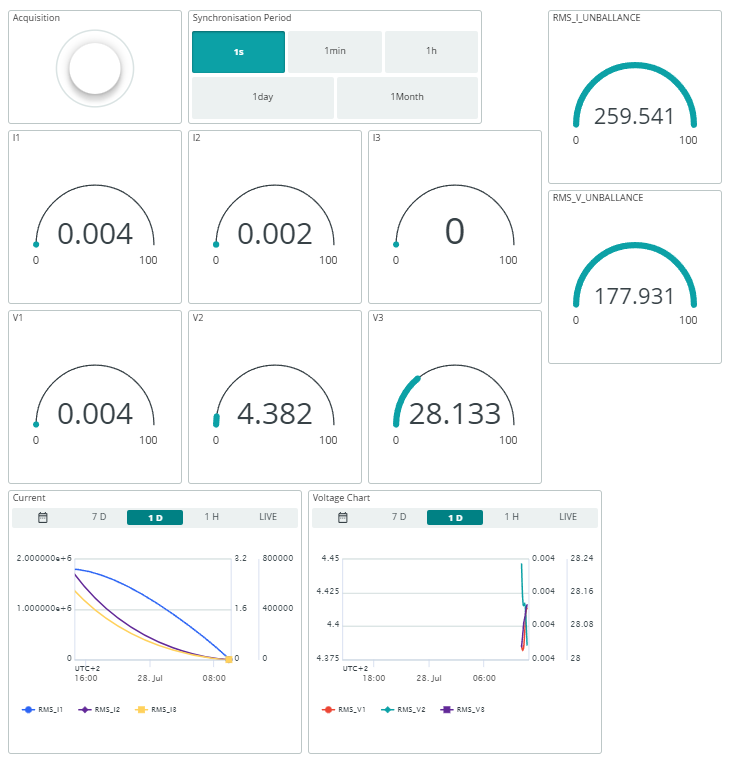
\includegraphics[scale=0.6]{images/Dashboard3.png}
\caption{Monitoring data through IoT Dashboard}
\label{fig:x IoT_Dashboard}
\end{figure}

This dynamic dashboard enables real-time monitoring of the three-phase currents (I1, I2, I3) and voltages (V1, V2, V3). Moreover, it offers intuitive graphical representations of historical data, enhancing data visualization. Notably, any instances of an unbalanced condition, expertly calculated by our system, are readily detectable through the RMS\_I\_UNBALANCE and RMS\_V\_UNBALANCE measurement units. These crucial values are meticulously computed and recorded through a dedicated local MATLAB script, overseen by our skilled engineers.



\chapter{Conclusion and Future Works}\label{Conclusion}
%\section{Conclusion and Future Works}
\section{Cost Analysis}
A simplified bill has been shown in Table \ref{tab:Cost Sheet}, where the total implementation cost of this acquisition board is calculated 137 euros only, which is really affordable.
\begin{table}[htbp]
  \centering
  \caption{Bill of Acquisition System Board }
  \label{tab:Cost Sheet}
  {
  \begin{tabular}{|c|c|c|}
    \hline
    \textbf{Particulars} & \textbf{Quantity} & \textbf{Price} \\
    \hline
     Arduino MKR 1500 & 1 & 60\texteuro \\
    \hline
    ADS131M08 ADC & 2 & 20\texteuro \\
    \hline
    Voltage Regulator & 5 & 5\texteuro \\
    \hline
    SMD Resistors & Lot & 5\texteuro \\
    \hline
    SMD Capacitors & Lot & 5\texteuro \\
    \hline
    SMD Diodes & 20 & 2\texteuro \\
    \hline
    M/F Connectors & Multiple & 5\texteuro \\
    \hline
    USB Connectors & 5 & 5\texteuro \\
    \hline
    Antenna Connector & 5 & 10\texteuro \\
    \hline
    PCB Board & 5 & 20\texteuro \\
    \hline
    \textbf{Total} & - & \textbf{137\texteuro} \\
    \hline
  \end{tabular}
  }
\end{table}

\section{Challenges Overcome} 
Throughout the implementation of this acquisition system, we encountered various challenges and adeptly surmounted each one. Designing precise signal conditioning circuits for ensuring accurate and noise-free signal acquisition posed a significant hurdle. Our efforts involved addressing common issues such as noise, interference, calibration, and offset. A particularly intricate task was generating a suitable clock for the ADC. Through resourceful adaptation of a \textbf{TurboPWM} library for SAMD21, we effectively overcame this challenge. Subsequent lab testing revealed a satisfactory \textbf{4KSPS} sampling rate, exceeding our expectations. Notably, the sampling duration for all eight channels amounted to a commendable \textbf{167ms}. Initially, we faced complications when attempting to execute the Simulink-generated embedded C files within our IDE. To resolve this matter, we successfully wrapped their declarations with \textbf{extern ‘C’ {}}. 

The Arduino MKR 1500 is equipped with 32KB of SRAM and 256KB of Flash RAM. Our project encountered challenges related to this 32KB memory limitation as we managed multiple threads and tasks within an RTOS framework. To address the memory constraint, we made the strategic decision to transmit selected sample packets to the cloud. While configuring NB-IoT proved relatively smooth, integrating it into our RTOS posed difficulties due to memory restrictions. Integrating the Arduino Cloud with MATLAB script required dedicated effort, particularly when writing data. Our perseverance paid off as we delved into the SDK support section of the Arduino Cloud, which offered valuable insights and solutions. However, a significant hurdle emerged when we sought to retrieve historical data from the Arduino Cloud. Initially, the platform lacked a direct option for accessing historical data. To overcome this, we embarked on an extensive study of various examples. Our endeavor bore fruit as we devised a MATLAB script that fulfilled this purpose, as previously discussed.

\section{Impact of this project for company} 
This initiative might have a big, encompassing influence on Schneider Electric. Numerous advantages and enhancements to Schneider's operations, goods, and services can result from such a system. Here are some potential impacts:\par
\vspace{0.5cm}
\textbf{Enhanced Monitoring and Control: }Schneider can monitor and manage numerous systems, pieces of equipment, and processes in real-time thanks to a powerful data collecting system. Better insights, quicker decision-making, and increased operational effectiveness result from this.
\par

\textbf{Predictive Maintenance:} Schneider may put into practice predictive maintenance techniques by gathering and processing data from essential equipment. As a result, downtime is decreased, equipment longevity is increased, and maintenance schedules are improved.
\par

\textbf{Data-Driven Insights:} This data collection system offers insightful information on equipment performance, operating trends, and energy usage patterns. With the aid of these insights, Schneider is able to provide its clients with data-driven solutions that assist them maximize their use of energy and operational effectiveness.
\par

\textbf{Remote Management:} Schneiders Engineers are able to remotely administer and monitor their systems installed at client locations. This makes it possible to debug, update, and customize more quickly without having to be physically there.
\par

\textbf{Product Development:} Schneider's goods and solutions may be designed and improved with the use of the collected data. It allows for iterative development based on actual usage data, producing more dependable and efficient services.
\par

\textbf{Energy Efficiency Solutions:} Schneider can create and offer energy management solutions that are specifically suited to the needs of its clients using the data it has collected. Reduced energy use, economic savings, and advantages for sustainability can result from this.
\par

\textbf{Business Growth:} A dependable data collecting system can improve Schneider's standing as a forward-thinking, technologically focused business. Through increased consumer attraction, business expansion, and the creation of new market opportunities.
\par

\textbf{Risk Management:} Monitoring essential devices and systems enables the early detection of possible difficulties before they grow into more serious concerns. The operational risks and possible interruptions are decreased by this proactive approach.
\par

\section{Future Works} 
The pursuit of knowledge knows no limitations, and we are ready to explore unexplored areas even more. With every obstacle we overcome, we find fresh opportunities just waiting to be explored. Future initiatives for our project have a lot of potential, as we can see. Potential directions include enhancing performance and adjusting the system to changing user requirements and market demands. The investigation of more sophisticated signal processing methods, such as filtering and noise reduction, promises to improve the quality of gathered data and provide insightful information as we move forward. Our agenda includes efficient memory management and needs that are specific to each user. Additionally, we see machine learning algorithms being integrated, allowing automation of anomaly detection, predictive maintenance, and pattern identification based on collected data.Furthermore, putting in place procedures for remote firmware updates guarantees that our system keeps up with the newest features, advancements, and security upgrades.





\phantomsection
\printbibliography % Where the bibliography will be printed
%\addcontentsline{toc}{chapter}{Bibliography}
% ********************************** Appendices ********************************
%\begin{appendices} % Using appendices environment for more functionality
%\newpage
\phantomsection

% ******************************* Thesis Appendix A ****************************
\chapter*{Appendix} 
\section*{Include}
\label{Firmware Include Files}
\begin{multicols}{3}
ADS131M08.h\par
Adafruit-SleepyDog.h\par
arduino-secrets.h\par
croutine.h\par
deprecated-definitions.h\par
error-hooks.h\par
event-groups.h\par
FreeRTOS-SAMD21.h\par
FreeRTOS.h\par
FreeRTOSConfig.h\par
list.h\par
message-buffer.h\par
mpu-prototypes.h\par
mpu-wrappers.h\par
portable.h\par
portmacro.h\par
projdefs.h\par
queue.h\par
runtimeStats-hooks.h\par
SAMD21turboPWM.h\par
semphr.h\par
stack-macros.h\par
stream-buffer.h\par
task.h\par
thingProperties.h\par
timers.h\par
\end{multicols}


\section*{Source}
\label{Firmware Source Files}
\begin{multicols}{3}
ADS131M08.cpp\par
croutine.c\par
error-hooks.cpp\par
event-groups.c\par
heap-4bis.c\par
list.c\par
port.c\par
queue.c\par
runTimeStats-hooks.c\par
SAMD21turboPWM.cpp\par
stream-buffer.c\par
task.c\par
timers.c\par
\end{multicols}

\section*{Main}
\label{Firmware Main}
\lstinputlisting[language=Octave]{main.cpp}
\section*{Matlab WebAccess}
\subsection*{Generating Authentication Token} \label{CREATING TOKEN}
\begin{lstlisting}[style=Matlab-Pyglike]
%:::::::::::::::CREATING TOKEN:::::::::::::::
opts_1 = weboptions('ContentType', 'json', 'Timeout',10)
url_token = 'https://api2.arduino.cc/iot/v1/clients/token';
response = webwrite(url_token,...
     'grant_type',  'client_credentials',...
     'client_id',   '5XXp84lsK8ACGKbU2bnWoUXYLVlkcquE',...
     'client_secret', '2WFU3ZALyHFg3yfWQpeqyKpfSzEMTXB7LnUZ6YynY9yygaAq8igICawa 4bdSDnvq',...
     'audience',    'https://api2.arduino.cc/iot',...
     opts_1);
access_token = response.access_token
\end{lstlisting}

\subsection*{Reading Data from Cloud}
\label{READING FROM CLOUD}
\begin{lstlisting}[style=Matlab-Pyglike]
%:::::::::::::::READING FROM CLOUD:::::::::::::::
url = 'https://api2.arduino.cc/iot/v2/things/';
Thing_Id = '25699f19-ee8a-4a0a-a7d3-028619992612';
RMS_I1 = "e72bf60d-ffe4-490a-bca5-ed3ad6f8450c";
RMS_I2 = "c091da24-c7a9-4368-ac73-5fa9bc590bac";
RMS_I3 = "cb5c8aee-4d39-42b9-91dc-8110acf761eb";
RMS_V1 = "f42c92af-7a1c-4423-941e-139fbe2691bb";
RMS_V2 = "a04faef9-ad2b-4f63-b4dd-e817a381eb01";
RMS_V3 = "6df1d034-e613-4695-81b8-7087d72f3c70";

url_request1 = strcat(url,Thing_Id,"/properties/",RMS_I1);
url_request2 = strcat(url,Thing_Id,"/properties/",RMS_I2);
url_request3 = strcat(url,Thing_Id,"/properties/",RMS_I3);

url_request4 = strcat(url,Thing_Id,"/properties/",RMS_V1);
url_request5 = strcat(url,Thing_Id,"/properties/",RMS_V2);
url_request6 = strcat(url,Thing_Id,"/properties/",RMS_V3);

opts_2 = weboptions('MediaType', 'auto',...
                     'HeaderFields', {'Authorization', ['Bearer ', access_token]});
%fieldValue = 42;
%for R = 1:20
%https://api2.arduino.cc/iot/v2/things/25699f19-ee8a-4a0a-a7d3-028619992612/properties/f06b9506-f7c8-473a-af4c-8b4dd028d455/publish
%url_request = "https://api2.arduino.cc/iot/v2/things/2332acc6-a929-4d1e-bfbc-00eb8518c2fb/properties/5695e3ea-5e49-4f2e-9804-48a500185f69";
    Variable1 = webread(url_request1, opts_2)
    Variable2 = webread(url_request2, opts_2)
    Variable3 = webread(url_request3, opts_2)
    Variable4 = webread(url_request4, opts_2)
    Variable5 = webread(url_request5, opts_2)
    Variable6 = webread(url_request6, opts_2)
 
I1 = Variable1.last_value
I2 = Variable2.last_value
I3 = Variable3.last_value

V1 = Variable4.last_value
V2 = Variable5.last_value
V3 = Variable6.last_value
%Variable_Last_Value = uint8(tmp);
%    pause(1);
\end{lstlisting}

\subsection*{Writting Data to the cloud}
\label{WRITTING TO THE CLOUD}
\begin{lstlisting}[style=Matlab-Pyglike]
%:::::::::::::::WRITTING TO THE CLOUD:::::::::::::::
url = "https://api2.arduino.cc/iot/v2";
Device_Id = "/155e65c7-5fe5-4a9c-bec1-5dccff54b206";
Thing_Id = "/25699f19-ee8a-4a0a-a7d3-028619992612";
Variable_Id = "/f06b9506-f7c8-473a-af4c-8b4dd028d455";


% Define the API endpoint and access token
url_request = strcat(url,"/things", Thing_Id,"/properties", Variable_Id, "/publish");


% Define the HTTP options
Headers = weboptions('HeaderFields', {'Authorization', ['Bearer ' access_token]},...
     'MediaType', 'application/json', ...
 'RequestMethod', 'put'); 

Body = struct('type', 'STRING',...
                'permission', 'READ_WRITE',...
                 'update_strategy','ON_CHANGE', ...
                 'value', 'Ahsan',...
                 'device_id', '155e65c7-5fe5-4a9c-bec1-5dccff54b206');


% Send the HTTP request
webwrite(url_request, Headers, Body)
\end{lstlisting}
\subsection*{Reading Historic Data}
\label{Historic Data}
\begin{lstlisting}[style=Matlab-Pyglike]
url = 'https://api2.arduino.cc/iot/v2/things/';
Thing_Id = '25699f19-ee8a-4a0a-a7d3-028619992612';
RMS_I1 = "e72bf60d-ffe4-490a-bca5-ed3ad6f8450c";
RMS_I2 = "c091da24-c7a9-4368-ac73-5fa9bc590bac";
RMS_I3 = "cb5c8aee-4d39-42b9-91dc-8110acf761eb";
RMS_V1 = "f42c92af-7a1c-4423-941e-139fbe2691bb";
RMS_V2 = "a04faef9-ad2b-4f63-b4dd-e817a381eb01";
RMS_V3 = "6df1d034-e613-4695-81b8-7087d72f3c70";

url_Var1 = strcat(url,Thing_Id,"/properties/",RMS_I1);
url_Var2 = strcat(url,Thing_Id,"/properties/",RMS_I2);
url_Var3 = strcat(url,Thing_Id,"/properties/",RMS_I3);

url_Var4 = strcat(url,Thing_Id,"/properties/",RMS_V1);
url_Var5 = strcat(url,Thing_Id,"/properties/",RMS_V2);
url_Var6 = strcat(url,Thing_Id,"/properties/",RMS_V3);
% Set the number of records you want to retrieve (optional)
Timeframe = "/timeseries?desc=1&from=2023-01-01T00:00:00Z&interval=1&to=2023-07-28T00:00:00Z"

url_request1 = strcat(url_Var1,Timeframe);
url_request2 = strcat(url_Var2,Timeframe);
url_request3 = strcat(url_Var3,Timeframe);
url_request4 = strcat(url_Var4,Timeframe);
url_request5 = strcat(url_Var5,Timeframe);
url_request6 = strcat(url_Var6,Timeframe);

opts_2 = weboptions('MediaType', 'auto',...
                     'HeaderFields', {'Authorization', ['Bearer ', access_token]});
%fieldValue = 42;
%for R = 1:20
%https://api2.arduino.cc/iot/v2/things/25699f19-ee8a-4a0a-a7d3-028619992612/properties/f06b9506-f7c8-473a-af4c-8b4dd028d455/publish
%url_request = "https://api2.arduino.cc/iot/v2/things/2332acc6-a929-4d1e-bfbc-00eb8518c2fb/properties/5695e3ea-5e49-4f2e-9804-48a500185f69";
    I1 = webread(url_request1,  opts_2)
    I2 = webread(url_request2, opts_2)
    I3 = webread(url_request3, opts_2)
    V1 = webread(url_request4, opts_2)
    V2 = webread(url_request5, opts_2)
    V3 = webread(url_request6, opts_2)

%Variable_Last_Value = uint8(tmp);
%    pause(1);



%:::::::::::::::READING and WRITTING TO THE CLOUD:::::::::::::::
url = 'https://api2.arduino.cc/iot/v2/things/';
Thing_Id = "1509add6-7574-4f78-824f-15fd26ba62f3";

RMS_I1 = "e72bf60d-ffe4-490a-bca5-ed3ad6f8450c";
RMS_I2 = "c091da24-c7a9-4368-ac73-5fa9bc590bac";
RMS_I3 = "cb5c8aee-4d39-42b9-91dc-8110acf761eb";
RMS_V1 = "f42c92af-7a1c-4423-941e-139fbe2691bb";
RMS_V2 = "a04faef9-ad2b-4f63-b4dd-e817a381eb01";
RMS_V3 = "6df1d034-e613-4695-81b8-7087d72f3c70";

url_request1 = strcat(url,Thing_Id,"/properties/",RMS_I1);
url_request2 = strcat(url,Thing_Id,"/properties/",RMS_I2);
url_request3 = strcat(url,Thing_Id,"/properties/",RMS_I3);

url_request4 = strcat(url,Thing_Id,"/properties/",RMS_V1);
url_request5 = strcat(url,Thing_Id,"/properties/",RMS_V2);
url_request6 = strcat(url,Thing_Id,"/properties/",RMS_V3);

% Set the number of records you want to retrieve (optional)

opts_2 = weboptions('MediaType', 'auto',...
                     'HeaderFields', {'Authorization', ['Bearer ', access_token]});
%fieldValue = 42;
%for R = 1:20
%https://api2.arduino.cc/iot/v2/things/25699f19-ee8a-4a0a-a7d3-028619992612/properties/f06b9506-f7c8-473a-af4c-8b4dd028d455/publish
%url_request = "https://api2.arduino.cc/iot/v2/things/2332acc6-a929-4d1e-bfbc-00eb8518c2fb/properties/5695e3ea-5e49-4f2e-9804-48a500185f69";
    Variable1 = webread(url_request1,  opts_2);
    Variable2 = webread(url_request2, opts_2);
    Variable3 = webread(url_request3, opts_2);
    Variable4 = webread(url_request4, opts_2);
    Variable5 = webread(url_request5, opts_2);
    Variable6 = webread(url_request6, opts_2);
 
I1 = Variable1.last_value
I2 = Variable2.last_value
I3 = Variable3.last_value
V1 = Variable4.last_value
V2 = Variable5.last_value
V3 = Variable6.last_value

%post processing
I_vec = [I1 I2 I3]
I_unbalance = max(I_vec)/mean(I_vec)*100;  %  In percent

V_vec = [V1 V2 V3]
V_unbalance = max(V_vec)/mean(V_vec)*100;  %  In percent

%:::::::::::::::WRITTING TO THE CLOUD:::::::::::::::
url = "https://api2.arduino.cc/iot/v2";
Thing_Id = "1509add6-7574-4f78-824f-15fd26ba62f3";
RMS_I_UNBALLANCE = "54473414-49cc-4ae8-8056-089bcca0fe2a";
RMS_V_UNBALLANCE = "2b2408d6-7118-4a2e-b874-8636d1a70dba";

% Define the API endpoint and access token
url_PUT_I_UNBALANCED = strcat(url,"/things/", Thing_Id,"/properties/", RMS_I_UNBALLANCE, "/publish");
url_PUT_V_UNBALANCED = strcat(url,"/things/", Thing_Id,"/properties/", RMS_V_UNBALLANCE, "/publish");


% Define the HTTP options
Headers = weboptions('HeaderFields', {'Authorization', ['Bearer ' access_token]},...
     'MediaType', 'application/json', ...
 'RequestMethod', 'put'); 
%Put= I_unbalance
Body_I = struct('type', 'FLOAT',...
                'permission', 'READ_WRITE',...
                 'update_strategy','ON_CHANGE', ...
                 'value', V_unbalance);
%Put= V_unbalance
Body_V = struct('type', 'FLOAT',...
                'permission', 'READ_WRITE',...
                 'update_strategy','ON_CHANGE', ...
                 'value', I_unbalance);

% Send the HTTP request
webwrite(url_PUT_I_UNBALANCED, Headers, Body_I)
webwrite(url_PUT_V_UNBALANCED, Headers, Body_V)
\end{lstlisting}






%\end{appendices}

\end{document}